% @author nicolas.guelfi
% @date Tue Nov 05 17:26:22 CET 2013
%-------------------------------------------------------------------------------
% Copyright (c) 2013 University of Luxembourg.
% All rights reserved. This program and the accompanying materials
% are made available under the terms of the Eclipse Public License v1.0
% which accompanies this distribution, and is available at
% http://www.eclipse.org/legal/epl-v10.html
% 
% Contributors:
%     Alfredo Capozucca - initial API and implementation
%     Benoit Ries - minor updates
%     Nicolas Guelfi - most content from messirbook
%-------------------------------------------------------------------------------
%%%%%%%%%%%%%%%%%%%%%%%%%%%%%%%%%%%%%%%%%%%%%%%%%%
\PassOptionsToPackage{usenames,svgnames,table}{xcolor}
\documentclass[graybox,envcountchap,sectrefs,11pt]{book} 
%%%%%%%%%%%%%%%%%%%%%%%%%%%%%%%%%%%%%%%%%%%%%%%%%%
%%% DO NOT CHANGE THE ORDER
\usepackage{./../lu.uni.lassy.excalibur.standard.report.libraries/styles/style-messir-common}
\usepackage{./../lu.uni.lassy.excalibur.standard.report.libraries/styles/style-messir-report-post}
%--------------------------------------------
% DOCUMENT BEGIN
%---------------------------------------- ----
\begin{document}

\newgeometry{textwidth=17cm,textheight=23.7cm} 

\newcommand{\msrReportType}{\emph{Report type: Default}~} 

  

\definecolor{lightgray}{RGB}{201,201,201}
\definecolor{lightred}{RGB}{250,112,97}
\definecolor{lightgreen}{RGB}{179,250,140}

\definecolor{msrtextcl}{RGB}{0,0,0}
\definecolor{msrkeycl}{RGB}{127,0,85}
\definecolor{msrcmtcl}{RGB}{201,201,201}
\definecolor{keywordcolor}{RGB}{30,144,255}

\definecolor{aqua_blue}{RGB}{0,139,145}
\definecolor{dark_green}{RGB}{0,128,0}
\definecolor{dark_blue}{RGB}{45,45,138}

\definecolor{msrcolor01}{rgb}{0.96,0.59,0.48}
\definecolor{msrcolor02}{rgb}{1.00,0.97,0.60}
\definecolor{msrcolor03}{rgb}{0.51,0.79,0.61}
\definecolor{msrcolor04}{rgb}{0.43,0.81,0.96}
\definecolor{msrcolor05}{rgb}{0.52,0.58,0.79}
\definecolor{msrcolor06}{rgb}{0.96,0.61,0.76}
\definecolor{msrcolor07}{rgb}{0.98,0.68,0.51}
\definecolor{msrcolor08}{rgb}{0.77,0.88,0.61}
\definecolor{msrcolor09}{rgb}{0.49,0.66,0.85}
\definecolor{msrcolor10}{rgb}{0.96,0.60,0.62}
\definecolor{msrcolor11}{rgb}{0.64,0.83,0.61}
\definecolor{msrcolor12}{rgb}{0.63,0.53,0.75}
\definecolor{msrcolor13}{rgb}{0.99,0.78,0.54}
\definecolor{msrcolor14}{rgb}{0.53,0.51,0.74}
\definecolor{msrcolor15}{rgb}{0.48,0.80,0.79}
\definecolor{msrcolor16}{rgb}{0.74,0.55,0.75}
\definecolor{msrcolor17}{rgb}{0.90,0.79,0.08}
\definecolor{msrcolor18}{rgb}{1.00,1.00,0.00}
\definecolor{msrcolor19}{rgb}{1.00,0.00,0.50}

\definecolor{sepcolor000000}{rgb}{0, 0, 0}
\definecolor{sepcolor101010}{rgb}{0.10, 0.10, 0.10}
\definecolor{sepcolor202020}{rgb}{0.20, 0.20, 0.20}
\definecolor{sepcolor303030}{rgb}{0.30, 0.30, 0.30}
\definecolor{sepcolor404040}{rgb}{0.10, 0.10, 0.10}
\definecolor{sepcolor505050}{rgb}{0,1,.5}
\definecolor{sepcolor907908}{rgb}{0,1,.5}

\definecolor{sepregioncolor01}{rgb}{0.00,0.66,0.00}
\definecolor{sepregioncolor02}{rgb}{1.00,1.00,0.00}
\definecolor{sepregioncolor03}{rgb}{1.00,0.97,0.60}
\definecolor{sepregioncolor04}{rgb}{0.64,0.83,0.61}
\definecolor{sepregioncolor05}{rgb}{0.95,0.36,0.00}
\definecolor{sepregioncolor06}{rgb}{0.90,0.79,0.08}
\definecolor{sepregioncolor07}{rgb}{0.63,0.53,0.75}
\definecolor{sepregioncolor08}{rgb}{0.99,0.78,0.54}
\definecolor{sepregioncolor09}{rgb}{0.96,0.61,0.76}
\definecolor{sepregioncolor10}{rgb}{1.00,0.00,0.50}

\colorlet{msrcolorbrown}{red!40!black!80}


% Messir General
%----------------------------------------------------------

% quotePosition + quoteWidth + quotefillColor + quoteElement + quotedElement + allImageScale
\newcommand{\msrcallouted}[6]{
\scalebox{#1}{\parbox{\linewidth}{
  \begin{tikzpicture}
      \node [rectangle callout,callout relative pointer={#4},text width=#5,fill=#6,rounded corners] (tmpcall) at (0,0) {#3};
      \node at (tmpcall.pointer){#2};
  \end{tikzpicture}
}}
}

% Vresion wihtout scaling the quoted text
\pgfkeys{%
    /calloutquote/.cd,
    width/.code                   =  {\def\calloutquotewidth{#1}},
    position/.code                =  {\def\calloutquotepos{#1}}, 
    author/.code                  =  {\def\calloutquoteauthor{#1}},
    /calloutquote/.unknown/.code   =  {\let\searchname=\pgfkeyscurrentname
                                 \pgfkeysalso{\searchname/.try=#1,
    /tikz/\searchname/.retry=#1},\pgfkeysalso{\searchname/.try=#1,
                                  /pgf/\searchname/.retry=#1}}
                            }  

\newcommand\calloutquote[2][]{%
  \pgfqkeys{/calloutquote}{#1}
  \node [rectangle callout,callout relative pointer={\calloutquotepos},text width=\calloutquotewidth,/calloutquote/.cd,#1] (tmpcall) at (0,0) {#2};
  \node at (tmpcall.pointer){\calloutquoteauthor};    
}  
%----------------------------------------------------------
\newcommand{\msrTalkRD}[6]{
\freeblock{5}{#1}{#2}{
\begin{figure}
  \centering
  \includegraphics[width=#5]{images/various/descartes.pdf} 
\end{figure}
}
\freeblock{5}{#3}{#4}{
\scriptsize
\textit{#6}
}
}
\newcommand{\msrTalkGB}[6]{
\freeblock{5}{#1}{#2}{
\begin{figure}
  \centering
  \includegraphics[width=#5]{images/various/graham-bell.pdf} 
\end{figure}
}
\freeblock{5}{#3}{#4}{
\scriptsize
\textit{#6}
}
}
%----------------------------------------------------------

\newcommand{\msrQuestionSlide}[1]{
\begin{frame}[fragile]
\freeblock{5}{1}{4}{
\begin{figure}
  \centering
  \includegraphics[width=3cm]{images/various/3d-man-question-sit.pdf}
\end{figure}
}
\freeblock{10}{5}{3}{
\Large
\msrtxtclb{red}{\textit{#1}}
}
\end{frame}
}

%%%%%%%%%%%%%%%%%%%%%%%%%%%%%%%%%%%%%%%%%%%%%%%%%%

\DeclareRobustCommand{\msrfigure}[4]{
\begin{figure}[htbp]
%\centering
\scalebox{#1}{
{\begin{minipage}[c]{\linewidth}
\centering
#2
\end{minipage}
}}
\ifthenelse{\equal{#4}{}}
             {}
             {\caption{#4}}
\label{#3}
\end{figure}
}

\newcommand{\semitransp}[2][30]{\color{fg!#1}#2}
\newcommand*{\msrtechfont}{\fontfamily{ptm}\selectfont}

\DeclareRobustCommand{\msruml}{{\msrtechfont UML}~}
\DeclareRobustCommand{\msrocl}{{\msrtechfont OCL}~}
\DeclareRobustCommand{\msromg}{{\msrtechfont OMG}~}
\DeclareRobustCommand{\msrxtext}{{\msrtechfont Xtext}~}
\DeclareRobustCommand{\msremf}{{\msrtechfont EMF}~}
\DeclareRobustCommand{\msrcm}{\msrcode{{Concept Model}}~}

\DeclareRobustCommand{\msrapache}{{\msrtechfont Apache}~}
\DeclareRobustCommand{\msratlassian}{{\msrtechfont Atlassian}~}
\DeclareRobustCommand{\msrbamboo}{{\msrtechfont Bamboo}~}
\DeclareRobustCommand{\msrconfluence}{{\msrtechfont Confluence}~}
\DeclareRobustCommand{\msreclemma}{{\msrtechfont EclEmma}~}
\DeclareRobustCommand{\msreclipse}{{\msrtechfont Eclipse}~}
\DeclareRobustCommand{\msrsql}{{\msrtechfont SQL}~}
\DeclareRobustCommand{\msrjava}{{\msrtechfont Java}~}
\DeclareRobustCommand{\msrjavafx}{{\msrtechfont JavaFx}~}
\DeclareRobustCommand{\msrjira}{{\msrtechfont JIRA}~}
\DeclareRobustCommand{\msrjunit}{{\msrtechfont JUnit}~}
\DeclareRobustCommand{\msrlatex}{{\msrtechfont Latex}~}
\DeclareRobustCommand{\msrmaven}{{\msrtechfont Maven}~}
\DeclareRobustCommand{\msrmysql}{{\msrtechfont MySQL}~}
\DeclareRobustCommand{\msrocl}{{\msrtechfont OCL}~}
\DeclareRobustCommand{\msrpdf}{{\msrtechfont PDF}~} 
\DeclareRobustCommand{\msrsirius}{{\msrtechfont Sirius}~} 
\DeclareRobustCommand{\msrsvn}{{\msrtechfont SubVersioN}~}
\DeclareRobustCommand{\msrswtbot}{{\msrtechfont SWTbot}~}
\DeclareRobustCommand{\msrxtext}{{\msrtechfont Xtext}~} 

 
\DeclareRobustCommand{\msrmessirmeth}{{\msrmessir}~methodology~}
\newcommand{\msrglsstyle}[1]{\emph{#1}}
\DeclareRobustCommand{\msrucname}[1]{\msrcode{\underline{#1}}}

% Verify macro since creates .toc errors
%\DeclareRobustCommand{\msrcode}[1]{{\normalfont\fontfamily{pcrr}\selectfont #1}}
%\DeclareRobustCommand{\msrcode}[1]{{\normalfont\fontfamily{cmvtt}\selectfont #1}}
\DeclareRobustCommand{\msrcode}[1]{{\protect\ \ttfamily \hyphenchar\font=`\- #1}}

% Messir Lexique
\DeclareRobustCommand{\msrbool}{\msrcode{{\emph Boolean}}~}
\DeclareRobustCommand{\msrint}{\msrcode{{\emph Integer}}~}
\DeclareRobustCommand{\msrreal}{\msrcode{{\emph Real}}~}
\DeclareRobustCommand{\msrstring}{\msrcode{{\emph String}}~}
\DeclareRobustCommand{\msrenum}{\msrcode{{\emph enumeration}}~}
\DeclareRobustCommand{\msrenums}{\msrcode{{\emph enumerations}}~}

% Messir Analysis
\DeclareRobustCommand{\msrsysop}{\emph{system operation}}
\DeclareRobustCommand{\msrsysops}{\emph{system operations}}
\DeclareRobustCommand{\msrsysintpro}{\emph{system interaction protocol}}
\DeclareRobustCommand{\msrbhvmd}{\emph{system operation}}

\newcommand{\msrt}[1]{\textuncl{#1}~}

\DeclareRobustCommand{\msrfont}[1]{\textuncl{#1}}
\DeclareRobustCommand{\msrfontb}[1]{\msrfont{\textbf{#1}}}
\DeclareRobustCommand{\msrfontcl}[1]{\msrfont{{\color{MediumPurple}#1}}}
\DeclareRobustCommand{\msrfontclb}[1]{{\msrfontcl{\textbf{#1}}}}

\DeclareRobustCommand{\msrcl}[1]{{\color{MediumPurple}#1}~}
\DeclareRobustCommand{\msrclb}[1]{{\msrcl{\textbf{#1}}}}

\DeclareRobustCommand{\msrmessir}{\msrfont{Messir}~}
\DeclareRobustCommand{\msrmessirb}{\msrfont{\textbf{Messir}}}
\DeclareRobustCommand{\msrmessircl}{{\color{MediumPurple}\msrmessir}}
\DeclareRobustCommand{\msrmessirclb}{{\color{MediumPurple}\msrmessirb}}

\DeclareRobustCommand{\msrexcalibur}{{\unclfamily Excalibur}~}
\DeclareRobustCommand{\msrexcaliburb}{\msrfont{\textbf{\msrexcalibur}}}
\DeclareRobustCommand{\msrexcaliburcl}{\msrfontcl{\msrexcalibur}}
\DeclareRobustCommand{\msrexcaliburclb}{\msrfontclb{\msrexcalibur}}

\DeclareRobustCommand{\msrmessim}{\msrfont{MesSim}}
\DeclareRobustCommand{\msrmessimb}{\msrfontb{MesSim}}
\DeclareRobustCommand{\msrmessimcl}{\msrfontcl{MesSim}}
\DeclareRobustCommand{\msrmessimclb}{\msrfontclb{MesSim}}

\DeclareRobustCommand{\msrmessam}{\msrfont{MesSam}}
\DeclareRobustCommand{\msrmessamb}{\msrfontb{MesSam}}
\DeclareRobustCommand{\msrmessamcl}{\msrfontcl{MesSam}}
\DeclareRobustCommand{\msrmessamclb}{\msrfontclb{MesSam}}

\DeclareRobustCommand{\msrmevop}{\msrfont{MevoP}~}
\DeclareRobustCommand{\msrmevopb}{\msrfontb{MevoP}~}
\DeclareRobustCommand{\msrmevopcl}{\msrfontcl{MevoP}~}
\DeclareRobustCommand{\msrmevopclb}{\msrfontclb{MevoP}~}

\DeclareRobustCommand{\msrmessep}{\msrfont{Messep}~}
\DeclareRobustCommand{\msrmessepb}{\msrfontb{Messep}~}
\DeclareRobustCommand{\msrmessepcl}{\msrfontcl{Messep}~}
\DeclareRobustCommand{\msrmessepclb}{\msrfontclb{Messep}~}

\DeclareRobustCommand{\msrmessee}{\msrfont{MesSEE}~}
\DeclareRobustCommand{\msrmesseeb}{\msrfontb{MesSEE}~}
\DeclareRobustCommand{\msrmesseecl}{\msrfontcl{MesSEE}~}
\DeclareRobustCommand{\msrmesseeclb}{\msrfontclb{MesSEE}~}

\DeclareRobustCommand{\msrprolog}{{\msrtechfont Prolog}}
\DeclareRobustCommand{\msrmessimb}{\textbf{\msrmessim}}
\DeclareRobustCommand{\msrprologcl}{\textcolor{red}{\msrprolog}}
\DeclareRobustCommand{\msrprologclb}{\textbf{\msrprologcl}}

\DeclareRobustCommand{\msrmcl}{{\footnotesize \msrfont{mcl}}}
\DeclareRobustCommand{\msrmclb}{\msrfontb{\msrmcl}}
\DeclareRobustCommand{\msrmclclb}{\msrfontcl{\msrmclb}}
\DeclareRobustCommand{\msrmclcl}{\msrfontcl{\msrmcl}}

\DeclareRobustCommand{\msrmcltt}{\protect\ \msrmessir Constraint Language~}
\DeclareRobustCommand{\msrmessimtt}{\protect\ \msrmessir Simulator~}
\DeclareRobustCommand{\msrmessamtt}{\protect\ \msrmessir Abstract Machine~}

\DeclareRobustCommand{\generic}{\textbf{\textit{{\color{MediumPurple}generic}}}~} 
\DeclareRobustCommand{\msrhelloworld}{\textbf{\textit{{\color{MediumPurple}HelloWorld}}}~}
\DeclareRobustCommand{\msricrash}{\textbf{\textit{{\color{MediumPurple}iCrash}}}~} 
\DeclareRobustCommand{\msricrashmini}{\textbf{\textit{{\color{MediumPurple}iCrashMini}}}~}  

\DeclareRobustCommand{\msrtxtcl}[2]{{\color{#1}#2}}
\DeclareRobustCommand{\msrtxtclb}[2]{\msrtxtcl{#1}{\textbf{#2}}}


%---------TABLES TEMPLATE--------------

%\rowcolors{2}{gray!20}{}

\newcounter{itemtable}


\newenvironment{usecase}{\begin{longtable}{|p{0.10\textwidth}
p{0.90\textwidth}|} \hline} {\hline \end{longtable}}


\newenvironment{usecaseinstance}{\begin{longtable}{|p{0.05\textwidth}
p{0.95\textwidth}|} \hline}
{\hline \end{longtable}}


\newenvironment{actortable}{
\begin{longtable}{|p{0.10\textwidth} p{0.90\textwidth}|}
\hline \hline}
{\hline \end{longtable}}


\newenvironment{datadictionary}{
\begin{longtable}{|p{0.15\textwidth} p{0.85\textwidth}|}
\hline \hline}
{\hline \end{longtable}}


\newenvironment{associationtypes}{
\begin{longtable}{|p{0.15\textwidth} p{0.85\textwidth}|}
\hline \hline}
{\hline \end{longtable}}


\newenvironment{operationmodel}{
\setcounter{itemtable}{0}
\begin{longtable}{|p{0.10\textwidth} p{0.90\textwidth}|}
\hline \hline}
{\hline \end{longtable}}


\newenvironment{teststepmodel}{
\setcounter{itemtable}{0}
\begin{longtable}{|p{0.10\textwidth}|p{0.90\textwidth}|}
\hline}
{\hline \end{longtable}}


\newcommand*{\myfont}{\fontfamily{phv}\selectfont}


\newcommand\addheading[1]{
\hline
%\multicolumn{2}{|l|}{\cellcolor[gray]{0.9} \textbf{#1}} \\
\multicolumn{2}{|l|}{\textbf{\scshape #1}} \\
\hline \hline
\endfirsthead

\multicolumn{2}{@{}l}{\myfont{\bfseries\itshape{\ldots #1 table
continuation}}}\\
%\hline \hline
%\multicolumn{2}{|l|}{\cellcolor[gray]{0.9} \textbf{#1}}\\
%\hline \hline
\endhead % all the lines above this will be repeated on every page

%\hline \hline
\multicolumn{2}{r@{}}{\myfont{\bfseries\itshape{continues in next page
\ldots}}}\\
\endfoot

\hline
\endlastfoot}

%\multicolumn{2}{|l|}{\cellcolor[gray]{0.8}
\newcommand\addrowheading[1]{
\hline \hline
\multicolumn{2}{|l|}{
  \setcounter{itemtable}{0}
  \textbf{\itshape #1}}\\
\hline \hline
}


\newcommand\addsinglerow[1]{
\multicolumn{2}{|l|}{\begin{minipage}[t][][t]{1.0\textwidth}
#1 \end{minipage}} \\
%\hline
}


\newcommand\addsingletwocolumnrow[2]{
{\itshape #1} & #2 \\
%\hline
}


\newcommand\adddoublerow[2]{
\hline \hline
\multicolumn{2}{|l|}{\begin{minipage}[t][][t]{1.0\textwidth}
\textbf{\itshape #1} \end{minipage}} \\
\multicolumn{2}{|l|}{\begin{minipage}[t][][t]{1.0\textwidth}
#2 \end{minipage}} \\
\hline
}


\newcommand\adddoubletwocolumnrow[3]{
#1 & \textbf{#2} \\
& #3 \\
%\hline
}


\newcommand\addnumberedsinglerow[2]{
\stepcounter{itemtable}
\text{#1 \theitemtable} & #2 \\
%\hline
}


\newcommand\addnumbereddoublerow[3]{
\stepcounter{itemtable}
\text{#1 \theitemtable} & \textbf{#2} \\
       & #3 \\
%\hline
}



\newcommand\addalphanumberedsinglerow[2]{
\stepcounter{itemtable}
\text{#1 \alph{itemtable}} & #2 \\
%\hline
}


\newcommand\addalphanumbereddoublerow[3]{
\stepcounter{itemtable}
\text{#1 \alph{itemtable}} & \textbf{#2} \\
       & #3 \\
%\hline
}

%%%%%%%%%%%%%%%%%%%%%%%%%%%%%%%%%%%%%%%%%%%%%%%%%%%%%%%%%%%%%%%%%%%%%%%%%%%%
%%%%%%%%%%%%%%%%%%%%%%%%%%%%%%%%%%%%%%%%%%%%%%%%%%%%%%%%%%%%%%%%%%%%%%%%%%%%

\lstdefinelanguage{MessirProlog}{
morekeywords=[1]{msrNav,msrop,:-},
morekeywords=[2]{msrVar},
morekeywords=[3]{msrTrue,msrFalse,true,false,msrIsNew,msrIsKilled,msrForAll,msrExists,msrSelect,msrReject,msrClose,msrAny,msrIsEmpty,msrSize,msmAtPre,msmAtPost,msrColEq,msrColSubtract,msrCount,msrExcludes,msrExcludesAll,msrIncludes,msrIncludesAll,msrSum,msrProd,msrIncluding,msrExcluding,msrIntersection,msrUnion,msrAsSet,msrOne},
morekeywords=[3]{rnSystem,rnActor,rnSystem,rnInterfaceIN,rnInterfaceOUT,ptBoolean,ptReal,ptString,ptInteger,preProtocol,preFunctional,postProtocol,postFunctional,init},
morekeywords=[4]{Self},
sensitive=true,
morestring=[b]{"},
comment=[s]{/*}{*/},
morecomment=[l]//
}[keywords,comments,strings]%
 
\lstdefinestyle{MessirPrologStyle} { 
language=MessirProlog,
extendedchars=true,
basicstyle=\ttfamily,
%keywordstyle=\color{blue}\bfseries,
keywordstyle=[1]\color{blue}\bfseries,
keywordstyle=[2]\color{red},
keywordstyle=[3]\color{msrcolor12}\bfseries,
keywordstyle=[4]\color{msrcolor09}\bfseries,
stringstyle=\color{msrtextcl},
commentstyle=\color{msrcmtcl},
breakatwhitespace=false,
tabsize=1,
literate={\ \ }{{\ }}1,
breaklines=true,
emptylines=1,
numbers=left,
numberstyle=\tiny\color{blue}, 
firstnumber=auto,
stepnumber=1,
numbersep=0pt, 
showspaces=false,
showlines=false,
numberfirstline=true,
showstringspaces=false
showtabs=false,
includerangemarker=true
}



\lstdefinestyle{MessirStyle} { 
language=Messir,
extendedchars=true,
basicstyle=\ttfamily,
keywordstyle=\color{msrkeycl}\bfseries,
stringstyle=\color{msrtextcl},
commentstyle=\color{msrcmtcl},
breakatwhitespace=false,
tabsize=1,
literate={\ \ }{{\ }}1,
breaklines=true,
emptylines=1,
numbers=left,
numberstyle=\tiny\bfseries\color{blue}, 
firstnumber=auto,
stepnumber=1,
numbersep=2pt, 
showspaces=false,
showlines=false,
numberfirstline=true,
showstringspaces=false
showtabs=false,
includerangemarker=true
}

\lstdefinelanguage{Messir}{
keywords={package,import,Concept,Model,Primary,Types,Secondary,state,class,
role,cardinality,extends,attribute,external,operation,primitive,
datatype,enum,constants,association,aggregation,composition,Environment,
actor,role,input,interface,output,Operation,external,link,preF,preP,postF,
postP,ocl,Test,test,case,order,step,prolog},
morekeywords=[1]{self,let,in,true,false,result},
morekeywords=[2]{name,attributes,associatoinEnds,operations,%
      supertypes,allSupertypes,allInstances,oclIsKindOf,oclIsTypeOf,%
      oclAsType,oclInState,oclIsNew,evaluationType,abs,floor,round,max,%
      min,div,mod,size,concat,toUpper,toLower,substring,includes,%
      excludes,count,includesAll,exludesAll,isEmpty,notEmpty,sum,%
      exists,forAll,isUnique,sortedBy,iterate,union,intersection,%
      including,excluding,symmetricDifference,select,reject,collect,%
      asSequence,asBag,asSequence,asSet,append,prepend,subSequence,at,%
      first,last,true,false,isQuery,context,pre,inv,post},
    morekeywords=[3]{and,equiv,exit,impl,not,or},%
    morekeywords=[4]{Boolean,Integer,Real,String,Set,Sequence,Bag,%
       OclType,OclAny,OclExpression,Enumeration,Collection},%
    morekeywords=[5]{Use,use,system,Case,Model,related,instance,primary,secondary,oracle,value,constraint,message,parameter,value,truth,protocol,functional,variables,values,results,subfunction,usergoal,summary,executes,sends,to,reuse,received,from,ordering,if,then,else,endif,self,^},
    morekeywords=[6]{executed,instanceof,returned,steps,active,passive,proactive,constraints,multiple},
    morekeywords=[7]{@Actor,@actorDeclaration,@actorSpecification,@additionalInformation,@attribute,@caption,@colOperation,@constraint,@description,@endActorsDeclaration,@endActorsSpecification,@endAttributes,@endColOperations,@endConstraints,@endInputEvents,@endInputParametersDeclaration,@endInputParametersSpecification,@endInstanceOracleOutputParameters,@endInstanceTestReceivedMessages,@endOperations,@endOracleConstraints,@endOracleOutputParametersSpecification,@endOracleReceivedMessagesSpecification,@endOracleValues,@endOracleVariables,@endOutputEvents,@endOutputParametersDeclaration,@endOutputParametersSpecification,@endParameters,@endPostConditions,@endPostF,@endPostP,@endPreConditions,@endPreF,@endPreP,@endProtocolConditions,@endRemarks,@endStepOrderingConstraints,@endVariables,@endVariableValues,@example,@inputEvent,@inputParameterDeclaration,@inputParameterSpecification,@Instance,@instanceOracleOutputParameter,@instanceTestReceivedMessage,@level,@model,@number,@Operation,@oracleConstraint,@oracleOutputParameterSpecification,@oracleReceivedMessageSpecification,@oracleSpecification,@oracleTruthValue,@oracleValue,@oracleVariable,@orientation,@outputEvent,@parameter,@postCondition,@postF,@postP,@preCondition,@preF,@preP,@Primary,@protocolCondition,@remark,@return,@scale,@Secondary,@stepOrderingConstraint,@sublevel,@Test,@testResultPostFunctional,@testResultPreFunctional,@testResultPreProcotol,@testSentMessage,@testSentMessageValue,@Use,@variable,@variableValue,@view,@pre,@post},
    morekeywords=[8]{@@Use,@@Instance,@@Primary,@@Secondary,@@Actor,@@Operation,@@Test,@@Instance,@@view,@operation},
sensitive=true,
morestring=[b]{"},
comment=[s]{/*}{*/},
morecomment=[l]//
%alsodigit={.}
}[keywords,comments,strings]%
%%%%%%%%%%%%%%%%%%%%%%%%%%%%%%%%%%%%%%%%%%%%%%%%%%%%%%%%%%%%%%%%%%%%%%%%%%%%
%%%%%%%%%%%%%%%%%%%%%%%%%%%%%%%%%%%%%%%%%%%%%%%%%%%%%%%%%%%%%%%%%%%%%%%%%%%%

%%%%%%%%%%%%%%%%%%%%%%%%%%%%%%%%%%%%%%%%%%%%%%%%%%%%%%%%%%%%%%%%%
%%%%%%%%%%%%%%      150506    %%%%%%%%%%%%%%%%%%%%%%%%%%%%%%%%%%%
%%%%%%%%%%%%%%%%%%%%%%%%%%%%%%%%%%%%%%%%%%%%%%%%%%%%%%%%%%%%%%%%%

\DeclareRobustCommand{\msrsee}{software engineering environment~}

\newcommand\freeblock[4]{%
\begin{textblock}{#1}(#2,#3)
\begin{minipage}{\textwidth}
\setlength{\parindent}{0pt}%
\setlength{\parskip}{0.1cm}%
#4
\end{minipage}
\end{textblock}
}
 
\newcommand\addheadingPS[4]{
\hline
\multicolumn{2}{|l|}{\textbf{\scshape Process Step}} \\
\hline
\multicolumn{2}{|l|}{Phase: \msrclb{#1} - Iteration: \msrclb{#2} - Step: \msrclb{#3}}\\
\hline
\multicolumn{2}{|l|}{Name: \msrclb{#4}}\\
\hline \hline
\endfirsthead 

\multicolumn{2}{@{}l}{\myfont{\bfseries\itshape{\ldots #1 table
continuation}}}\\
\endhead % all the lines above this will be repeated on every page

\multicolumn{2}{r@{}}{\myfont{\bfseries\itshape{continues in next page
\ldots}}}\\
\endfoot

\hline
\endlastfoot}

\newenvironment{processsteptable}{
\setcounter{itemtable}{0}
\begin{longtable}{|p{0.10\textwidth}|p{0.90\textwidth}|}
\hline}
{\hline \end{longtable}
}

%%%%%%%%%%%%%%%%%%%%%%%%%%%%%%%%%%%%%%%%%%%%%%%%%%
\newcommand{\mybox}[2]{\par\noindent\colorbox{#1}
{\parbox{\dimexpr\textwidth-2\fboxsep\relax}{#2}}}

%for time line tables
\newcommand\ytl[5]{
\parbox[b]{8em}{\hfill{\color{#2}\bfseries\sffamily #3}~$\cdots\cdots$~}\makebox[0pt][c]{$\bullet$}\vrule\quad \parbox[c]{\textwidth}{\vspace{#1pt}\color{#4}\raggedright\sffamily #5\\[7pt]}\\[-3pt]}

% For setting item spacing
% ex: {\setlistspacing{2}{2ex} \begin{frame} \ldots \end{frame}}
\makeatletter
\newcommand{\setlistspacing}[2]{\def\@ld{#1}\expandafter\def\csname
@list\romannumeral\@ld \endcsname{\leftmargin\csname
leftmargin\romannumeral\@ld \endcsname
              \topsep    #2
              \parsep    0\p@   \@plus\p@
              \itemsep   #2}}
\makeatother




%  General Messir Glossary
\newglossaryentry{real number}
{name={real},
description={name of the set of real numbers},
plural={reals},
symbol={\ensuremath{\mathbb{R}}}
}

\newglossaryentry{systop}
{name={\msrglsstyle{system operation}},
description={a functionality of the system that can be triggered by a message sent by an actor belonging to the environment.},
plural={system operations},
symbol={\msrglsstyle{system operation}}
}

\newglossaryentry{protmod}
{name={\msrglsstyle{Protocol Model}},
description={},
plural={protocol models},
symbol={\msrglsstyle{protocol model}}
}

\newglossaryentry{societics}
{name={\msrglsstyle{Societics}},
description={Represents the fields of hardware/software
systems used for the society extension.},
symbol={\msrglsstyle{societics}}
}

\newglossaryentry{direct actor}
{name={\msrglsstyle{direct actor}},
description={an actor that interacts directly with the system. It thus belongs to the environment.},
plural={direct actors},
symbol={\msrglsstyle{direct actor}}
}

\newglossaryentry{indirect actor}
{name={\msrglsstyle{indirect actor}},
description={an actor that interacts indirectly with the system through a direct actor. It thus belongs the domain but not to the environment.},
plural={\msrglsstyle{indirect actors}},
symbol={\msrglsstyle{indirect actor}}
}

\newglossaryentry{abstract actor}
{name={\msrglsstyle{abstract actor}},
description={an actor that is not },
plural={\msrglsstyle{abstract actors}},
symbol={\msrglsstyle{abstract actor}}
}

\newglossaryentry{socext}
{name={\msrglsstyle{Society extension}},
description={The society obtained by grouping people using natural means
extended with artificial means.},
symbol={\msrglsstyle{societics}} }

\newglossaryentry{usecase}
{name={\msrglsstyle{Use case}},
description={A use case describes a sequence of actions that provide something
of measurable value to an actor. and is drawn as a horizontal ellipse.},
symbol={\msrglsstyle{Use case}} 
plural={\msrglsstyle{Use cases}} }

\newglossaryentry{actor}
{name={\msrglsstyle{actor}},
description={An actor is a person, organization, or external system that plays a role in one or more interactions with the system},
plural={actors},
symbol={\msrglsstyle{actor}}
}

\newglossaryentry{socialware}
{name={\msrglsstyle{Societics}},
description={Represents the fields of hardware/software
systems used for the society extension.},
symbol={\msrglsstyle{Societics}}
}

\newglossaryentry{system operation}
{name={system operation},
description={a functionality of the system that can be triggered by a message sent by an actor belonging to the environment.},
plural={system operation},
symbol={\msrglsstyle{system operation}}
}




% \newglossaryentry{}
% {name={\msrglsstyle{}},
% description={},
% symbol={\msrglsstyle{actor}} }

\newcommand{\msrprojectname}{\emph{icrash}~} 

\newcommand{\msrReportAuthors}{} 

\newcommand{\msrReportAffiliation}{
\begin{tabular}{l}
        Laboratory for Advanced Software Systems\\
        University of Luxembourg\\
\end{tabular}
} 

\newcommand{\msrReportTitle}{
\begin{tabular}{|>{\centering\arraybackslash\hspace{0pt}}p{12cm}|}
\hline
    \textbf{\msricrash:}\\
    \textbf{A Crisis Management Case Study}\\
    \textbf{\msrmessirclb Analysis Document}\\
    \textbf{ - v 1.4 - }\\
    \vspace{.5cm}
    {\large(\msrReportType) }\\
\hline
\end{tabular}
}
  

%TITLE
%******************************************
\title{
\freeblock{10}{2}{5}{
\scalebox{1.3}{\parbox{\linewidth}{
\msrReportTitle}
}}
\vspace{2cm}
\freeblock{5}{10}{-.8}{
\begin{figure}
  \centering
  \includegraphics[width=6cm,natwidth=5847,natheight=7135]{./../lu.uni.lassy.excalibur.standard.report.libraries/logos/Messir-no-OS-focused.eps} 
\end{figure}
}
\freeblock{5}{12.5}{-.8}{
\begin{figure}
  \centering
  \includegraphics[width=5.63cm,natwidth=5256,natheight=6852]{./../lu.uni.lassy.excalibur.standard.report.libraries/logos/Excalibur-no-OS-focused.eps}
\end{figure}
\freeblock{5}{1}{1.5}{
\scalebox{.9}{\parbox{\linewidth}{
\msrReportAffiliation
\msrReportAuthors
}}}
\freeblock{10}{5}{10}{
\scalebox{.9}{\parbox{\linewidth}{
\today~-~\currenttime
}}}
}
}
%******************************************
\author{}

\date{}
%****************************************************


\maketitle
\newpage

%TOC
\setcounter{tocdepth}{2}
\addtocounter{secnumdepth}{2}
\tableofcontents
\newpage

%TOF
\listoffigures
\newpage

%TOL
\lstlistoflistings
\newpage

%DOCUMENT STRUCTURE
% Last Modification:
% @author AUTHOR_NAME
% @date TODAY_DATE

\chapter{Introduction}
\label{chap:introduction}
\newpage

% Last Modification:
% @author AUTHOR_NAME
% @date TODAY_DATE

\chapter{General Description}
\label{chap:general_description}
\newpage

%\section{Use Cases Model}
\label{sec:lu.uni.lassy.excalibur.examples.icrash-gendescr-usecasemodel}

This section contains the use cases elicited during the requirements elicitation phase.
The use cases are textually described as suggested by the \msrmessir method and inspired by the standard Cokburn template~\cite{armour01usecase}.


%% ***************************************************************
%% Use Cases
\subsection{Use Cases}



%% ***************************************************************
%% Summary Use Cases

\subsubsection{summary-suDeployAndRun}

\label{RE-use-case-suDeployAndRun}


The goal is to install the iCrash system on its infrastructure and to exploit its capacities related to the secure administration and efficient handling of car crash situations depending on alerts received. 


\begin{usecase}
  \addheading{Use-Case Description}
  \addsingletwocolumnrow{Name}{suDeployAndRun}
  \addsingletwocolumnrow{Scope}{system}
  \addsingletwocolumnrow{Level}{summary}
  

\addrowheading{Primary actor(s)}
\addnumberedsinglerow{}{\msrcode{actAdministrator[active]}}


\addrowheading{Secondary actor(s)}
\addnumberedsinglerow{}{\msrcode{actMsrCreator[active]}}
\addnumberedsinglerow{}{\msrcode{actCoordinator[active, multiple]}}
\addnumberedsinglerow{}{\msrcode{actActivator[proactive]}}
\addnumberedsinglerow{}{\msrcode{actComCompany[active]}}

\addrowheading{Goal(s) description}
\addsinglerow{The goal is to install the iCrash system on its infrastructure and to exploit its capacities related to the secure administration and efficient handling of car crash situations depending on alerts received. 
}

\addrowheading{Reuse}
\addnumberedsinglerow{}{\msrucname{oeCreateSystemAndEnvironment [1..1]}}
\addnumberedsinglerow{}{\msrucname{ugAdministrateTheSystem [1..*]}}
\addnumberedsinglerow{}{\msrucname{suGlobalCrisisHandling [1..*]}}
\addnumberedsinglerow{}{\msrucname{oeSetClock [1..*]}}
\addnumberedsinglerow{}{\msrucname{oeSollicitateCrisisHandling [0..*]}}
\addnumberedsinglerow{}{\msrucname{oeAlert [1..*]}}

\addrowheading{Protocol condition(s)}
\addnumberedsinglerow{}{
the iCrash system has never been deployed and used
}

\addrowheading{Pre-condition(s)}
\addnumberedsinglerow{}{
none
}

\addrowheading{Main post-condition(s)}
\addnumberedsinglerow{}{
the iCrash system has been created and has handled the crisis situations for which it received alerts through the communication company.
}

\addrowheading{Main Steps}
\addalphanumberedsinglerow{}{the actor \msrcode{actMsrCreator} executes the \msrucname{oeCreateSystemAndEnvironment} use case}
\addalphanumberedsinglerow{}{the actor \msrcode{actAdministrator} executes the \msrucname{ugAdministrateTheSystem} use case}
\addalphanumberedsinglerow{}{the actor \msrcode{actComCompany} executes the \msrucname{oeAlert} use case}
\addalphanumberedsinglerow{}{the actor \msrcode{actActivator} executes the \msrucname{oeSetClock} use case}
\addalphanumberedsinglerow{}{the actor \msrcode{actActivator} executes the \msrucname{oeSollicitateCrisisHandling} use case}
\addalphanumberedsinglerow{}{the actor \msrcode{actCoordinator} executes the \msrucname{suGlobalCrisisHandling} use case}
\addrowheading{Steps Ordering Constraints}
\addnumberedsinglerow{}{step (a) must be always the first step.}
\addnumberedsinglerow{}{step (f) can be executed by different actCoordinator actors.}
\addnumberedsinglerow{}{if (e) then previously (d).}


\end{usecase} 


Figure \ref{fig:lu.uni.lassy.excalibur.examples.icrash-RE-UCD-uc-suDeployAndRun}
shows the use case diagram for the suDeployAndRun summary use case

\begin{figure}[htbp]
\begin{center}

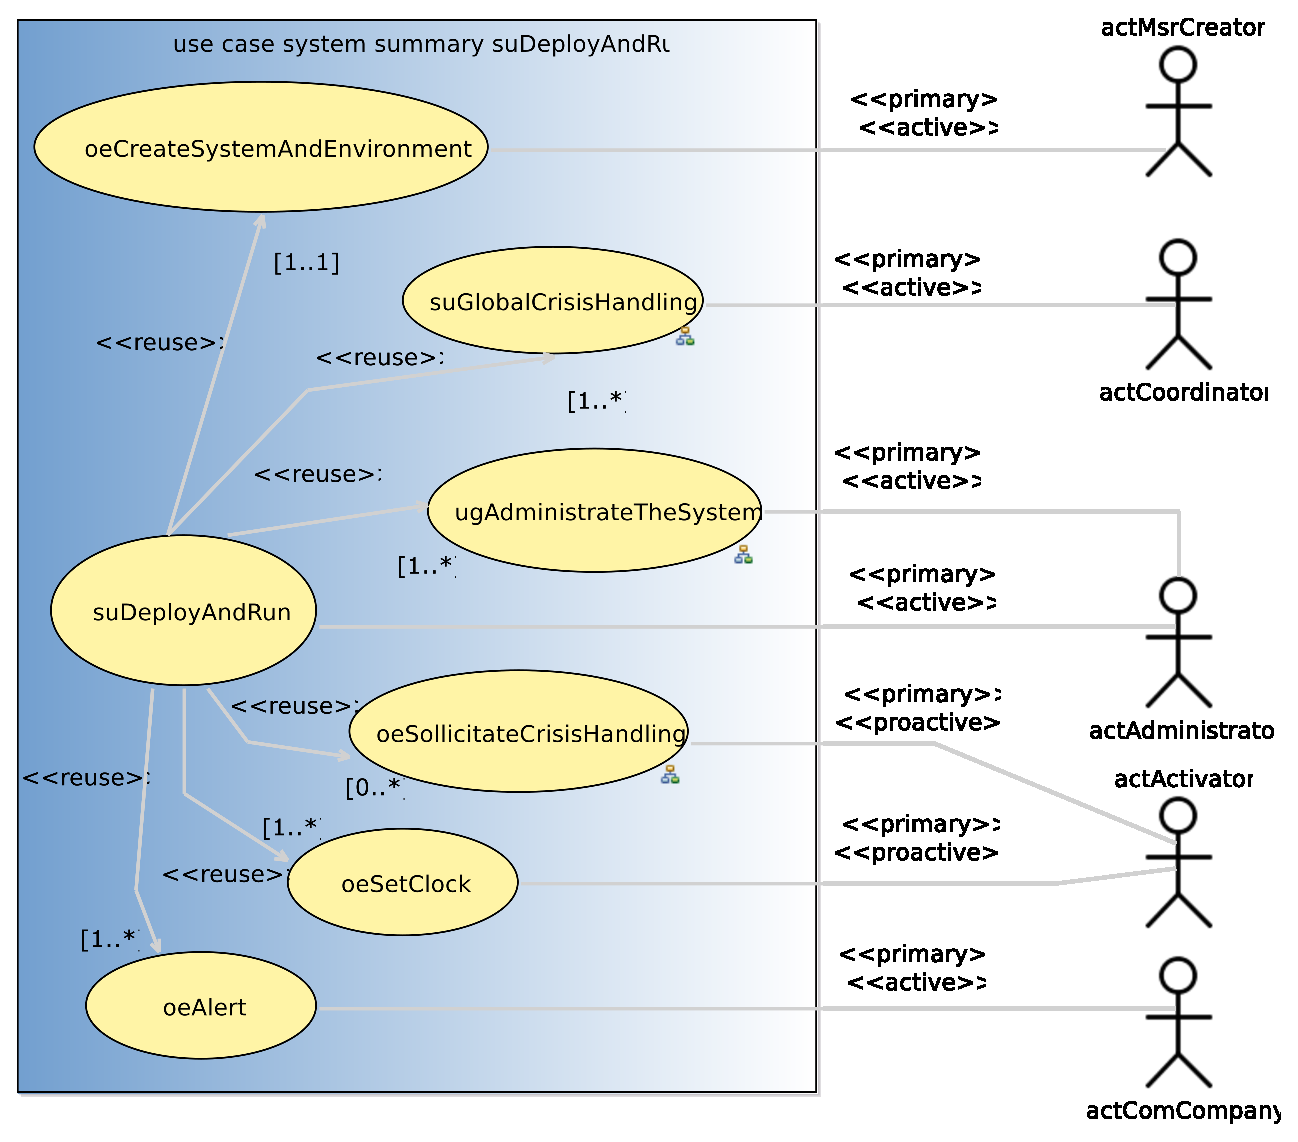
\includegraphics[
angle=0
,width=1.0\textwidth
]{./images-report-gen/usecase-model/summary/uc-suDeployAndRun.eps}
\end{center}
\caption[lu.uni.lassy.excalibur.examples.icrash Use Case Diagram: uc-suDeployAndRun]{ suDeployAndRun summary use case}
\label{fig:lu.uni.lassy.excalibur.examples.icrash-RE-UCD-uc-suDeployAndRun}
\end{figure}
\vspace{0.5cm}

\subsubsection{summary-suGlobalCrisisHandling}

\label{RE-use-case-suGlobalCrisisHandling}


the actCoordinator's goal is to monitor the alerts received and the corresponding crisis in order to act as necessary to handle the crisis. 		  


\begin{usecase}
  \addheading{Use-Case Description}
  \addsingletwocolumnrow{Name}{suGlobalCrisisHandling}
  \addsingletwocolumnrow{Scope}{system}
  \addsingletwocolumnrow{Level}{summary}
  

\addrowheading{Primary actor(s)}
\addnumberedsinglerow{}{\msrcode{actCoordinator[active]}}



\addrowheading{Goal(s) description}
\addsinglerow{the actCoordinator's goal is to monitor the alerts received and the corresponding crisis in order to act as necessary to handle the crisis. }

\addrowheading{Reuse}
\addnumberedsinglerow{}{\msrucname{ugSecurelyUseSystem [1..*]}}
\addnumberedsinglerow{}{\msrucname{ugMonitor [1..*]}}
\addnumberedsinglerow{}{\msrucname{ugManageCrisis [1..*]}}

\addrowheading{Protocol condition(s)}
\addnumberedsinglerow{}{ the iCrash system has been deployed}
\addnumberedsinglerow{}{the coordinator actor involded in the use case has been declared by the actor actAdministrator}

\addrowheading{Pre-condition(s)}
\addnumberedsinglerow{}{none}

\addrowheading{Main post-condition(s)}
\addnumberedsinglerow{}{ modifications have been made by the coordinator on existing alerts or crisis OR the coordinator requested an updated status on existing alerts or crisis.}

\addrowheading{Main Steps}
\addalphanumberedsinglerow{}{the actor \msrcode{actCoordinator} executes the \msrucname{ugSecurelyUseSystem} use case}
\addalphanumberedsinglerow{}{the actor \msrcode{actCoordinator} executes the \msrucname{ugMonitor} use case}
\addalphanumberedsinglerow{}{the actor \msrcode{actCoordinator} executes the \msrucname{ugManageCrisis} use case}
\addrowheading{Steps Ordering Constraints}
\addnumberedsinglerow{}{steps (a) (b) and (c) executions are interleaved 
        (steps (b) and (c) have their protocol constrained by steps of (a)).}
\addnumberedsinglerow{}{steps (a) (b) and (c) can be executed multiple times.}


\end{usecase} 


Figure \ref{fig:lu.uni.lassy.excalibur.examples.icrash-RE-UCD-uc-suGlobalCrisisHandling}
shows the use case diagram for the suGlobalCrisisHandling user goal use case

\begin{figure}[htbp]
\begin{center}

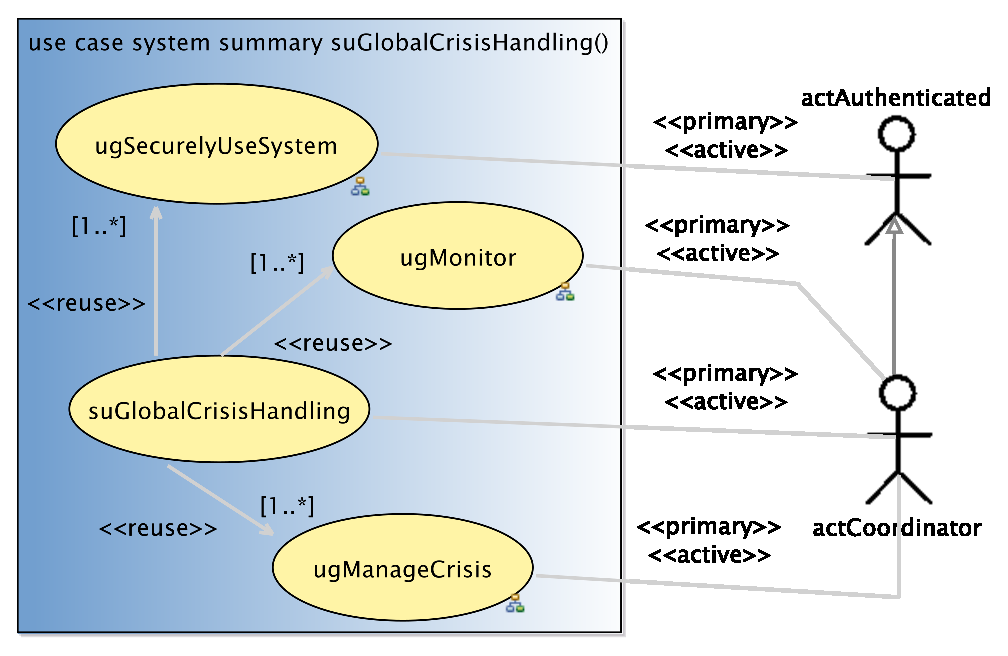
\includegraphics[
angle=0
,scale=0.75
]{./images-report-gen/usecase-model/summary/uc-suGlobalCrisisHandling.eps}
\end{center}
\caption[lu.uni.lassy.excalibur.examples.icrash Use Case Diagram: uc-suGlobalCrisisHandling]{ suGlobalCrisisHandling user goal use case}
\label{fig:lu.uni.lassy.excalibur.examples.icrash-RE-UCD-uc-suGlobalCrisisHandling}
\end{figure}
\vspace{0.5cm}



%% ***************************************************************
%% User-Goal Use Cases
\subsubsection{usergoal-ugAdministrateTheSystem}

\label{RE-use-case-ugAdministrateTheSystem}



the actAdministrator's goal is to follow an identification procedure to be allowed to add or delete the necessary crisis coordinators that will be granted the responsibility to handle alerts and crisis. 


\begin{usecase}
  \addheading{Use-Case Description}
  \addsingletwocolumnrow{Name}{ugAdministrateTheSystem}
  \addsingletwocolumnrow{Scope}{system}
  \addsingletwocolumnrow{Level}{usergoal}
  

\addrowheading{Primary actor(s)}
\addnumberedsinglerow{}{\msrcode{actAdministrator[active]}}



\addrowheading{Goal(s) description}
\addsinglerow{
the actAdministrator's goal is to follow an identification procedure to be allowed to add or delete the necessary crisis coordinators that will be granted the responsibility to handle alerts and crisis. 
}

\addrowheading{Reuse}
\addnumberedsinglerow{}{\msrucname{ugSecurelyUseSystem [1..*]}}
\addnumberedsinglerow{}{\msrucname{oeAddCoordinator [1..*]}}
\addnumberedsinglerow{}{\msrucname{oeDeleteCoordinator [0..*]}}

\addrowheading{Protocol condition(s)}
\addnumberedsinglerow{}{
the iCrash system has been deployed
}

\addrowheading{Pre-condition(s)}
\addnumberedsinglerow{}{
none
}

\addrowheading{Main post-condition(s)}
\addnumberedsinglerow{}{
modifications have been made to the system and its environment concerning existing or new coordinators.
}

\addrowheading{Main Steps}
\addalphanumberedsinglerow{}{the actor \msrcode{actAdministrator} executes the \msrucname{ugSecurelyUseSystem} use case}
\addalphanumberedsinglerow{}{the actor \msrcode{actAdministrator} executes the \msrucname{oeAddCoordinator} use case}
\addalphanumberedsinglerow{}{the actor \msrcode{actAdministrator} executes the \msrucname{oeDeleteCoordinator} use case}
\addrowheading{Steps Ordering Constraints}
\addnumberedsinglerow{}{steps (a) (b) and (c) executions are interleaved 
          (steps (b) and (c) have their protocol constrained 
           by steps of (a)).}
\addnumberedsinglerow{}{steps (a) (b) and (c) can be executed multiple times.}


\end{usecase} 


Figure \ref{fig:lu.uni.lassy.excalibur.examples.icrash-RE-UCD-uc-ugAdministrateTheSystem}
shows the use case diagram for the ugAdministrateTheSystem user goal use case

\begin{figure}[htbp]
\begin{center}

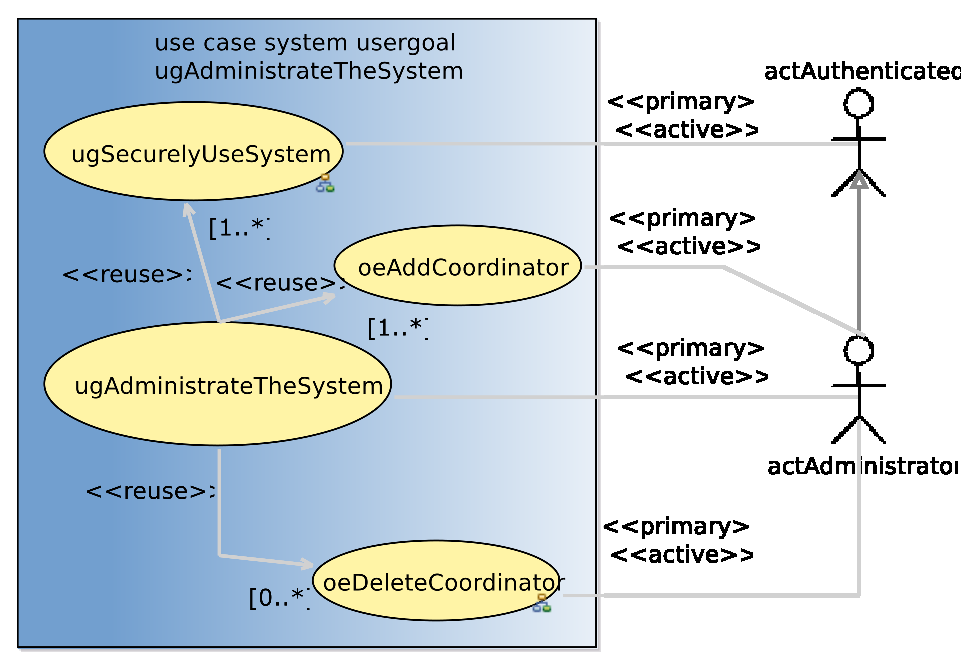
\includegraphics[
angle=0
,scale=0.75
]{./images-report-gen/usecase-model/usergoal/uc-ugAdministrateTheSystem.eps}
\end{center}
\caption[lu.uni.lassy.excalibur.examples.icrash Use Case Diagram: uc-ugAdministrateTheSystem]{ ugAdministrateTheSystem user goal use case}
\label{fig:lu.uni.lassy.excalibur.examples.icrash-RE-UCD-uc-ugAdministrateTheSystem}
\end{figure}
\vspace{0.5cm}

\subsubsection{usergoal-ugManageCrisis}

\label{RE-use-case-ugManageCrisis}



The goal is to do an action that makes the handling of a crisis or an alert progress. 


\begin{usecase}
  \addheading{Use-Case Description}
  \addsingletwocolumnrow{Name}{ugManageCrisis}
  \addsingletwocolumnrow{Scope}{system}
  \addsingletwocolumnrow{Level}{usergoal}
  

\addrowheading{Primary actor(s)}
\addnumberedsinglerow{}{\msrcode{actCoordinator[active]}}



\addrowheading{Goal(s) description}
\addsinglerow{
The goal is to do an action that makes the handling of a crisis or an alert progress. 
}

\addrowheading{Reuse}
\addnumberedsinglerow{}{\msrucname{oeValidateAlert [0..*]}}
\addnumberedsinglerow{}{\msrucname{oeSetCrisisStatus [0..*]}}
\addnumberedsinglerow{}{\msrucname{oeSetCrisisHandler [0..*]}}
\addnumberedsinglerow{}{\msrucname{oeReportOnCrisis [0..*]}}
\addnumberedsinglerow{}{\msrucname{oeCloseCrisis [0..*]}}
\addnumberedsinglerow{}{\msrucname{oeInvalidateAlert [0..*]}}

\addrowheading{Protocol condition(s)}
\addnumberedsinglerow{}{
the iCrash system has been deployed
}

\addrowheading{Pre-condition(s)}
\addnumberedsinglerow{}{
none
}

\addrowheading{Main post-condition(s)}
\addnumberedsinglerow{}{
there exist one alert or one crisis whose related information has been changed.
}

\addrowheading{Main Steps}
\addalphanumberedsinglerow{}{the actor \msrcode{actCoordinator} executes the \msrucname{oeValidateAlert} use case}
\addalphanumberedsinglerow{}{the actor \msrcode{actCoordinator} executes the \msrucname{oeSetCrisisStatus} use case}
\addalphanumberedsinglerow{}{the actor \msrcode{actCoordinator} executes the \msrucname{oeSetCrisisHandler} use case}
\addalphanumberedsinglerow{}{the actor \msrcode{actCoordinator} executes the \msrucname{oeReportOnCrisis} use case}
\addalphanumberedsinglerow{}{the actor \msrcode{actCoordinator} executes the \msrucname{oeCloseCrisis} use case}
\addalphanumberedsinglerow{}{the actor \msrcode{actCoordinator} executes the \msrucname{oeInvalidateAlert} use case}
\addrowheading{Steps Ordering Constraints}
\addnumberedsinglerow{}{managing a crisis is doing one of the indicated use cases.}


\end{usecase} 


Figure \ref{fig:lu.uni.lassy.excalibur.examples.icrash-RE-UCD-uc-ugManageCrisis}
shows the use case diagram for the ugManageCrisis user goal use case

\begin{figure}[htbp]
\begin{center}

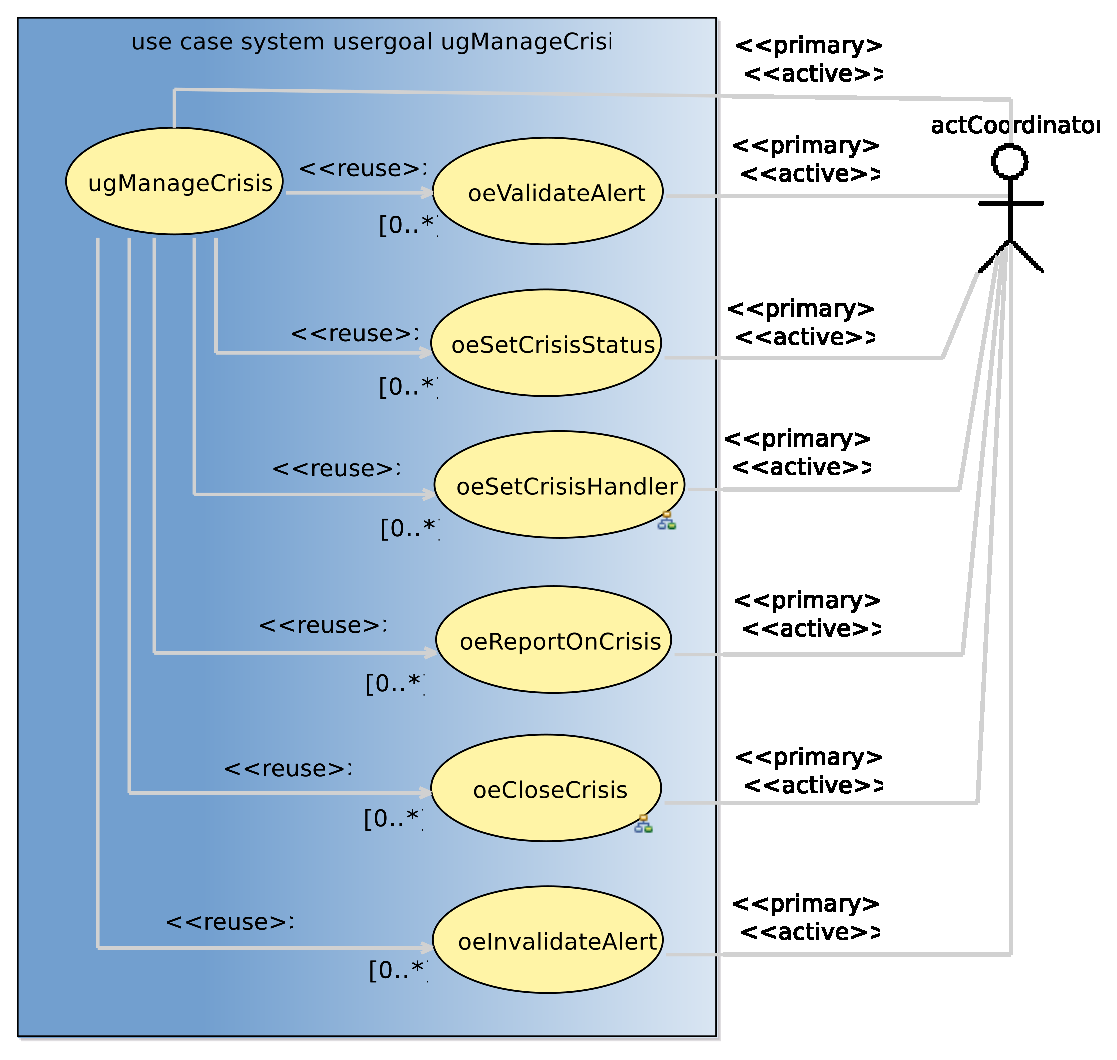
\includegraphics[
angle=0
,scale=0.75
]{./images-report-gen/usecase-model/usergoal/uc-ugManageCrisis.eps}
\end{center}
\caption[lu.uni.lassy.excalibur.examples.icrash Use Case Diagram: uc-ugManageCrisis]{ ugManageCrisis user goal use case}
\label{fig:lu.uni.lassy.excalibur.examples.icrash-RE-UCD-uc-ugManageCrisis}
\end{figure}
\vspace{0.5cm}

\subsubsection{usergoal-ugMonitor}

\label{RE-use-case-ugMonitor}



the actCoordinator's goal is to get the detailed list of existing crisis or alerts to decide on next actions to undertake. 


\begin{usecase}
  \addheading{Use-Case Description}
  \addsingletwocolumnrow{Name}{ugMonitor}
  \addsingletwocolumnrow{Scope}{system}
  \addsingletwocolumnrow{Level}{usergoal}
  

\addrowheading{Primary actor(s)}
\addnumberedsinglerow{}{\msrcode{actCoordinator[active]}}



\addrowheading{Goal(s) description}
\addsinglerow{
the actCoordinator's goal is to get the detailed list of existing crisis or alerts to decide on next actions to undertake. 
}

\addrowheading{Reuse}
\addnumberedsinglerow{}{\msrucname{oeGetCrisisSet [0..*]}}
\addnumberedsinglerow{}{\msrucname{oeGetAlertsSet [0..*]}}

\addrowheading{Protocol condition(s)}
\addnumberedsinglerow{}{
the iCrash system has been deployed
}

\addrowheading{Pre-condition(s)}
\addnumberedsinglerow{}{
none
}

\addrowheading{Main post-condition(s)}
\addnumberedsinglerow{}{
none
}

\addrowheading{Main Steps}
\addalphanumberedsinglerow{}{the actor \msrcode{actCoordinator} executes the \msrucname{oeGetAlertsSet} use case}
\addalphanumberedsinglerow{}{the actor \msrcode{actCoordinator} executes the \msrucname{oeGetCrisisSet} use case}


\end{usecase} 


Figure \ref{fig:lu.uni.lassy.excalibur.examples.icrash-RE-UCD-uc-ugMonitor}
shows the use case diagram for the ugMonitor user goal use case

\begin{figure}[htbp]
\begin{center}

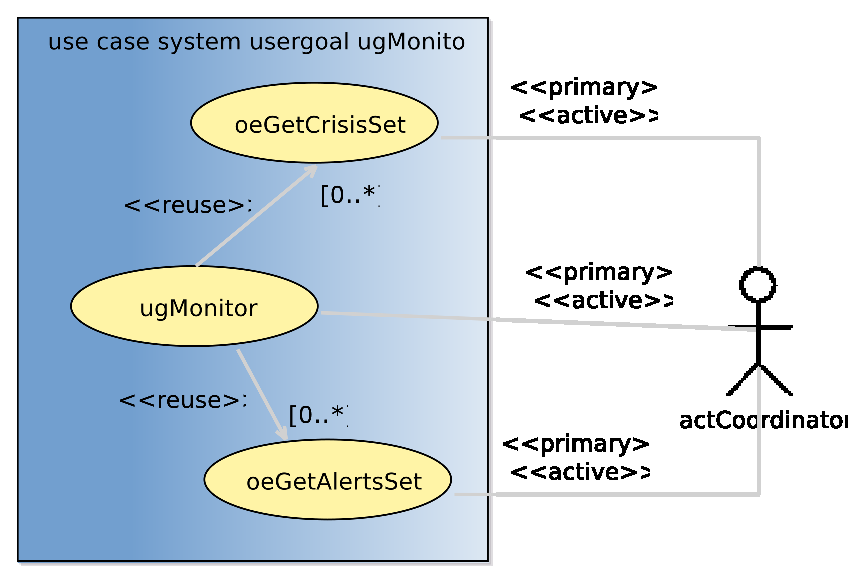
\includegraphics[
angle=0
,scale=0.75
]{./images-report-gen/usecase-model/usergoal/uc-ugMonitor.eps}
\end{center}
\caption[lu.uni.lassy.excalibur.examples.icrash Use Case Diagram: uc-ugMonitor]{ ugMonitor user goal use case}
\label{fig:lu.uni.lassy.excalibur.examples.icrash-RE-UCD-uc-ugMonitor}
\end{figure}
\vspace{0.5cm}

\subsubsection{usergoal-ugSecurelyUseSystem}

\label{RE-use-case-ugSecurelyUseSystem}



the actAdministrator's goal is to follow an identification procedure to be allowed to add or delete the necessary crisis coordinators that will be granted the responsibility to handle alerts and crisis. 


\begin{usecase}
  \addheading{Use-Case Description}
  \addsingletwocolumnrow{Name}{ugSecurelyUseSystem}
  \addsingletwocolumnrow{Scope}{system}
  \addsingletwocolumnrow{Level}{usergoal}
  

\addrowheading{Primary actor(s)}
\addnumberedsinglerow{}{\msrcode{actAuthenticated[active]}}



\addrowheading{Goal(s) description}
\addsinglerow{
the actAdministrator's goal is to follow an identification procedure to be allowed to add or delete the necessary crisis coordinators that will be granted the responsibility to handle alerts and crisis. 
}

\addrowheading{Reuse}
\addnumberedsinglerow{}{\msrucname{oeLogin [1..1]}}
\addnumberedsinglerow{}{\msrucname{oeLogout [1..1]}}

\addrowheading{Protocol condition(s)}
\addnumberedsinglerow{}{
the iCrash system has been deployed
}

\addrowheading{Pre-condition(s)}
\addnumberedsinglerow{}{
none
}

\addrowheading{Main post-condition(s)}
\addnumberedsinglerow{}{
the actAuthenticated is known by the system not to be logged.
}

\addrowheading{Main Steps}
\addalphanumberedsinglerow{}{the actor \msrcode{actAuthenticated} executes the \msrucname{oeLogin} use case}
\addalphanumberedsinglerow{}{the actor \msrcode{actAuthenticated} executes the \msrucname{oeLogout} use case}
\addrowheading{Steps Ordering Constraints}
\addnumberedsinglerow{}{step (a) must always precede step (b).}


\end{usecase} 


Figure \ref{fig:lu.uni.lassy.excalibur.examples.icrash-RE-UCD-uc-ugSecurelyUseSystem}
shows the use case diagram for the ugSecurelyUseSystem user goal use case

\begin{figure}[htbp]
\begin{center}

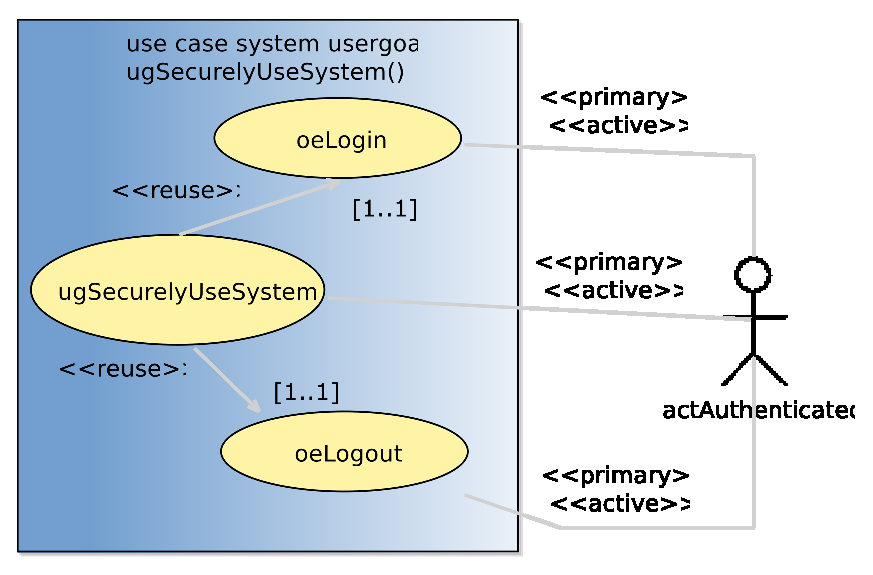
\includegraphics[
angle=0
,scale=0.75
]{./images-report-gen/usecase-model/usergoal/uc-ugSecurelyUseSystem.eps}
\end{center}
\caption[lu.uni.lassy.excalibur.examples.icrash Use Case Diagram: uc-ugSecurelyUseSystem]{ ugSecurelyUseSystem user goal use case}
\label{fig:lu.uni.lassy.excalibur.examples.icrash-RE-UCD-uc-ugSecurelyUseSystem}
\end{figure}
\vspace{0.5cm}



%% ***************************************************************
%% Subfunction Use Cases
\subsubsection{subfunction-oeDeleteCoordinator}

\label{RE-use-case-oeDeleteCoordinator}


Figure \ref{fig:lu.uni.lassy.excalibur.examples.icrash-RE-UCD-uc-oeDeleteCoordinator}

\begin{figure}[htbp]
\begin{center}

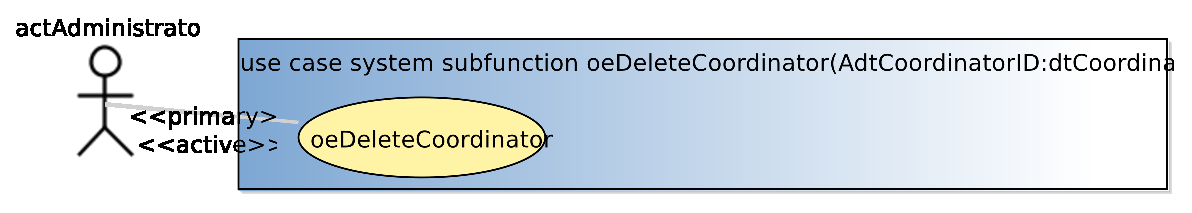
\includegraphics[
angle=0
]{./images-report-gen/usecase-model/subfunction/uc-oeDeleteCoordinator.eps}
\end{center}
\caption[lu.uni.lassy.excalibur.examples.icrash Use Case Diagram: uc-oeDeleteCoordinator]{}
\label{fig:lu.uni.lassy.excalibur.examples.icrash-RE-UCD-uc-oeDeleteCoordinator}
\end{figure}
\vspace{0.5cm}

\subsubsection{subfunction-oeRecoveryPassword}

\label{RE-use-case-oeRecoveryPassword}




\begin{usecase}
  \addheading{Use-Case Description}
  \addsingletwocolumnrow{Name}{oeRecoveryPassword}
  \addsingletwocolumnrow{Scope}{system}
  \addsingletwocolumnrow{Level}{subfunction}
  

\addrowheading{Primary actor(s)}
\addnumberedsinglerow{}{\msrcode{actAdministrator[active]}}



\addrowheading{Goal(s) description}
\addsinglerow{}

\addrowheading{Protocol condition(s)}
\addnumberedsinglerow{}{
}

\addrowheading{Pre-condition(s)}
\addnumberedsinglerow{}{
}

\addrowheading{Main post-condition(s)}
\addnumberedsinglerow{}{
}

\addrowheading{Additional Information}
\addsinglerow{
none
}

\end{usecase} 


\subsubsection{subfunction-oeSetCrisisHandler}

\label{RE-use-case-oeSetCrisisHandler}


goal is to declare himself as been the handler of a crisis having the specified id.


\begin{usecase}
  \addheading{Use-Case Description}
  \addsingletwocolumnrow{Name}{oeSetCrisisHandler}
  \addsingletwocolumnrow{Scope}{system}
  \addsingletwocolumnrow{Level}{subfunction}
  
\addrowheading{Parameters}
\addnumberedsinglerow{AdtCrisisID: dtCrisisID}{}

\addrowheading{Primary actor(s)}
\addnumberedsinglerow{}{\msrcode{actCoordinator[active]}}


\addrowheading{Secondary actor(s)}
\addnumberedsinglerow{}{\msrcode{actCoordinator[passive]}}
\addnumberedsinglerow{}{\msrcode{actComCompany[passive, multiple]}}

\addrowheading{Goal(s) description}
\addsinglerow{goal is to declare himself as been the handler of a crisis having the specified id.
}

\addrowheading{Protocol condition(s)}
\addnumberedsinglerow{}{
}

\addrowheading{Pre-condition(s)}
\addnumberedsinglerow{}{
}

\addrowheading{Main post-condition(s)}
\addnumberedsinglerow{}{
}

\addrowheading{Additional Information}
\addsinglerow{
none
}

\end{usecase} 

Figure \ref{fig:lu.uni.lassy.excalibur.examples.icrash-RE-UCD-uc-oeSetCrisisHandler}
shows the use case diagram for the oeSetCrisisHandler subfunction use case

\begin{figure}[htbp]
\begin{center}

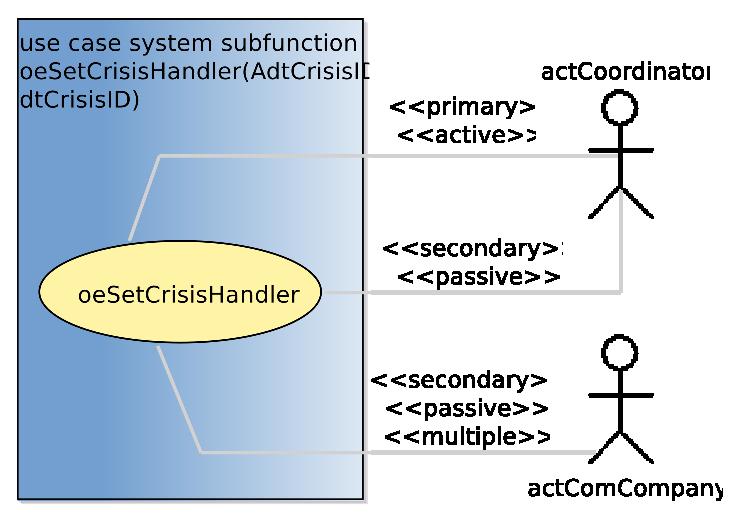
\includegraphics[
angle=0
,scale=0.75
]{./images-report-gen/usecase-model/subfunction/uc-oeSetCrisisHandler.eps}
\end{center}
\caption[lu.uni.lassy.excalibur.examples.icrash Use Case Diagram: uc-oeSetCrisisHandler]{oeSetCrisisHandler subfunction use case
}
\label{fig:lu.uni.lassy.excalibur.examples.icrash-RE-UCD-uc-oeSetCrisisHandler}
\end{figure}
\vspace{0.5cm}

\subsubsection{subfunction-oeSollicitateCrisisHandling}

\label{RE-use-case-oeSollicitateCrisisHandling}



the actActivator's goal is to decrease the number of unhandled crisis. 


\begin{usecase}
  \addheading{Use-Case Description}
  \addsingletwocolumnrow{Name}{oeSollicitateCrisisHandling}
  \addsingletwocolumnrow{Scope}{system}
  \addsingletwocolumnrow{Level}{subfunction}
  

\addrowheading{Primary actor(s)}
\addnumberedsinglerow{}{\msrcode{actActivator[proactive]}}


\addrowheading{Secondary actor(s)}
\addnumberedsinglerow{}{\msrcode{actCoordinator[passive, multiple]}}
\addnumberedsinglerow{}{\msrcode{actAdministrator[passive]}}

\addrowheading{Goal(s) description}
\addsinglerow{
the actActivator's goal is to decrease the number of unhandled crisis. 
}

\addrowheading{Protocol condition(s)}
\addnumberedsinglerow{}{
the iCrash system has been deployed.
}
\addnumberedsinglerow{}{
there exist some crisis still pending and for which no solicitation has been sent to the administrator and the coordinators for more than a predefined maximum delay.
}

\addrowheading{Pre-condition(s)}
\addnumberedsinglerow{}{
none
}

\addrowheading{Main post-condition(s)}
\addnumberedsinglerow{}{
a simple text message ieMessage('There are alerts not treated since more than the defined delay. Please REACT !\') is sent to the system administrator and to all the coordinators of the environment for each crisis that is known to be not handled and for which no solicitation has been sent to the administrator and the coordinators for more than a predefined maximum delay.')
}
\addnumberedsinglerow{}{
the reminder period for the concerned crisis is initialized.
}


\end{usecase} 

Figure \ref{fig:lu.uni.lassy.excalibur.examples.icrash-RE-UCD-uc-oeSollicitateCrisisHandling}
shows the use case diagram for the oeSollicitateCrisisHandling subfunction use case

\begin{figure}[htbp]
\begin{center}

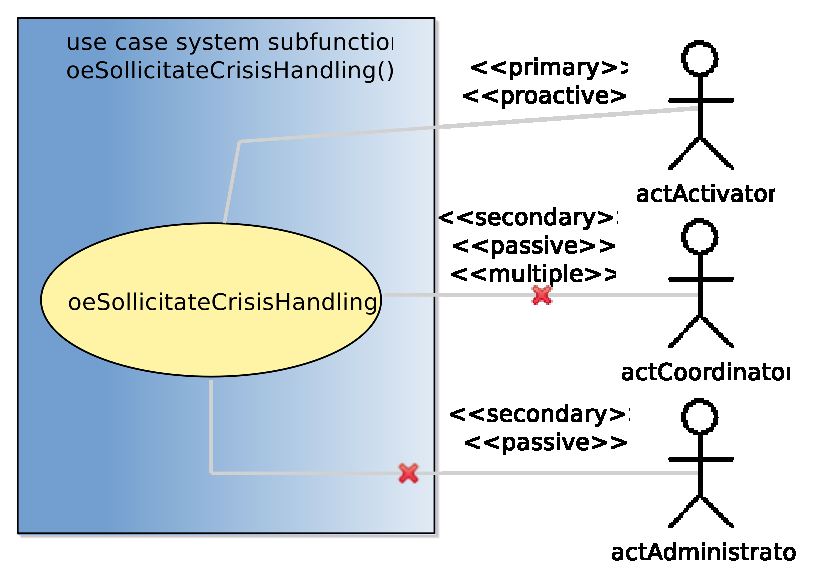
\includegraphics[
angle=0
,scale=0.75
]{./images-report-gen/usecase-model/subfunction/uc-oeSollicitateCrisisHandling.eps}
\end{center}
\caption[lu.uni.lassy.excalibur.examples.icrash Use Case Diagram: uc-oeSollicitateCrisisHandling]{ oeSollicitateCrisisHandling subfunction use case}
\label{fig:lu.uni.lassy.excalibur.examples.icrash-RE-UCD-uc-oeSollicitateCrisisHandling}
\end{figure}
\vspace{0.5cm}




%% ***************************************************************
%% Use Case Instances
\pagebreak
\subsection{Use Case Instance(s)}


%% ***************************************************************
%% Summary Use Case Instances

	\subsubsection{Use-Case Instance - uciSimpleAndCompletePart01:suDeployAndRun}
	
	First part of a use case instance for the summary use case \msrcode{suDeployAndRun} illustrating a simple and complete interaction scenario primarily handled by an administrator in a concrete situation.
	\begin{operationmodel}
	\addheading{summary Use-Case Instance}
	\adddoublerow{Instantiated Use Case}{suDeployAndRun}
	\adddoublerow{Instance ID}{uciSimpleAndCompletePart01}
	
	\addrowheading{Remarks}
	\addalphanumberedsinglerow{}{shows the system initilization and the first administrative tasks by the administrator. }
	\addalphanumberedsinglerow{}{The unique and always existing \msrcode{actMsrCreator} actor instance (named here \msrcode{theCreator}) requests the initialization of the system and its environment (made of one administrator identified here by \msrcode{bill}), one activator actor (identified by \msrcode{theClock}) and indicating that the number of communication company actor instances for the system's environment is 4 (one of them is identified here by \msrcode{tango})}
	\addalphanumberedsinglerow{}{the administrator logs in to initialize a coordinator}
	\addalphanumberedsinglerow{}{an alert is received. Time is goind one without having the coordinator handling the alert which let's the proactive actor trigger the automatic sollicitation of crisis handling.}
	\addalphanumberedsinglerow{}{this first part stops before the coordinator logs in the system.}
	\end{operationmodel} 

	
	Figure \ref{fig:lu.uni.lassy.excalibur.examples.icrash-RE-UC-uci-suDeployAndRun-uciSimpleAndComplete-Part01}
	shows the sequence diagram representing the first part of a simple and complete use case instance for the summary use case \msrcode{suDeployAndRun}.
	
	\begin{figure}[htbp]
	\begin{center}
	
	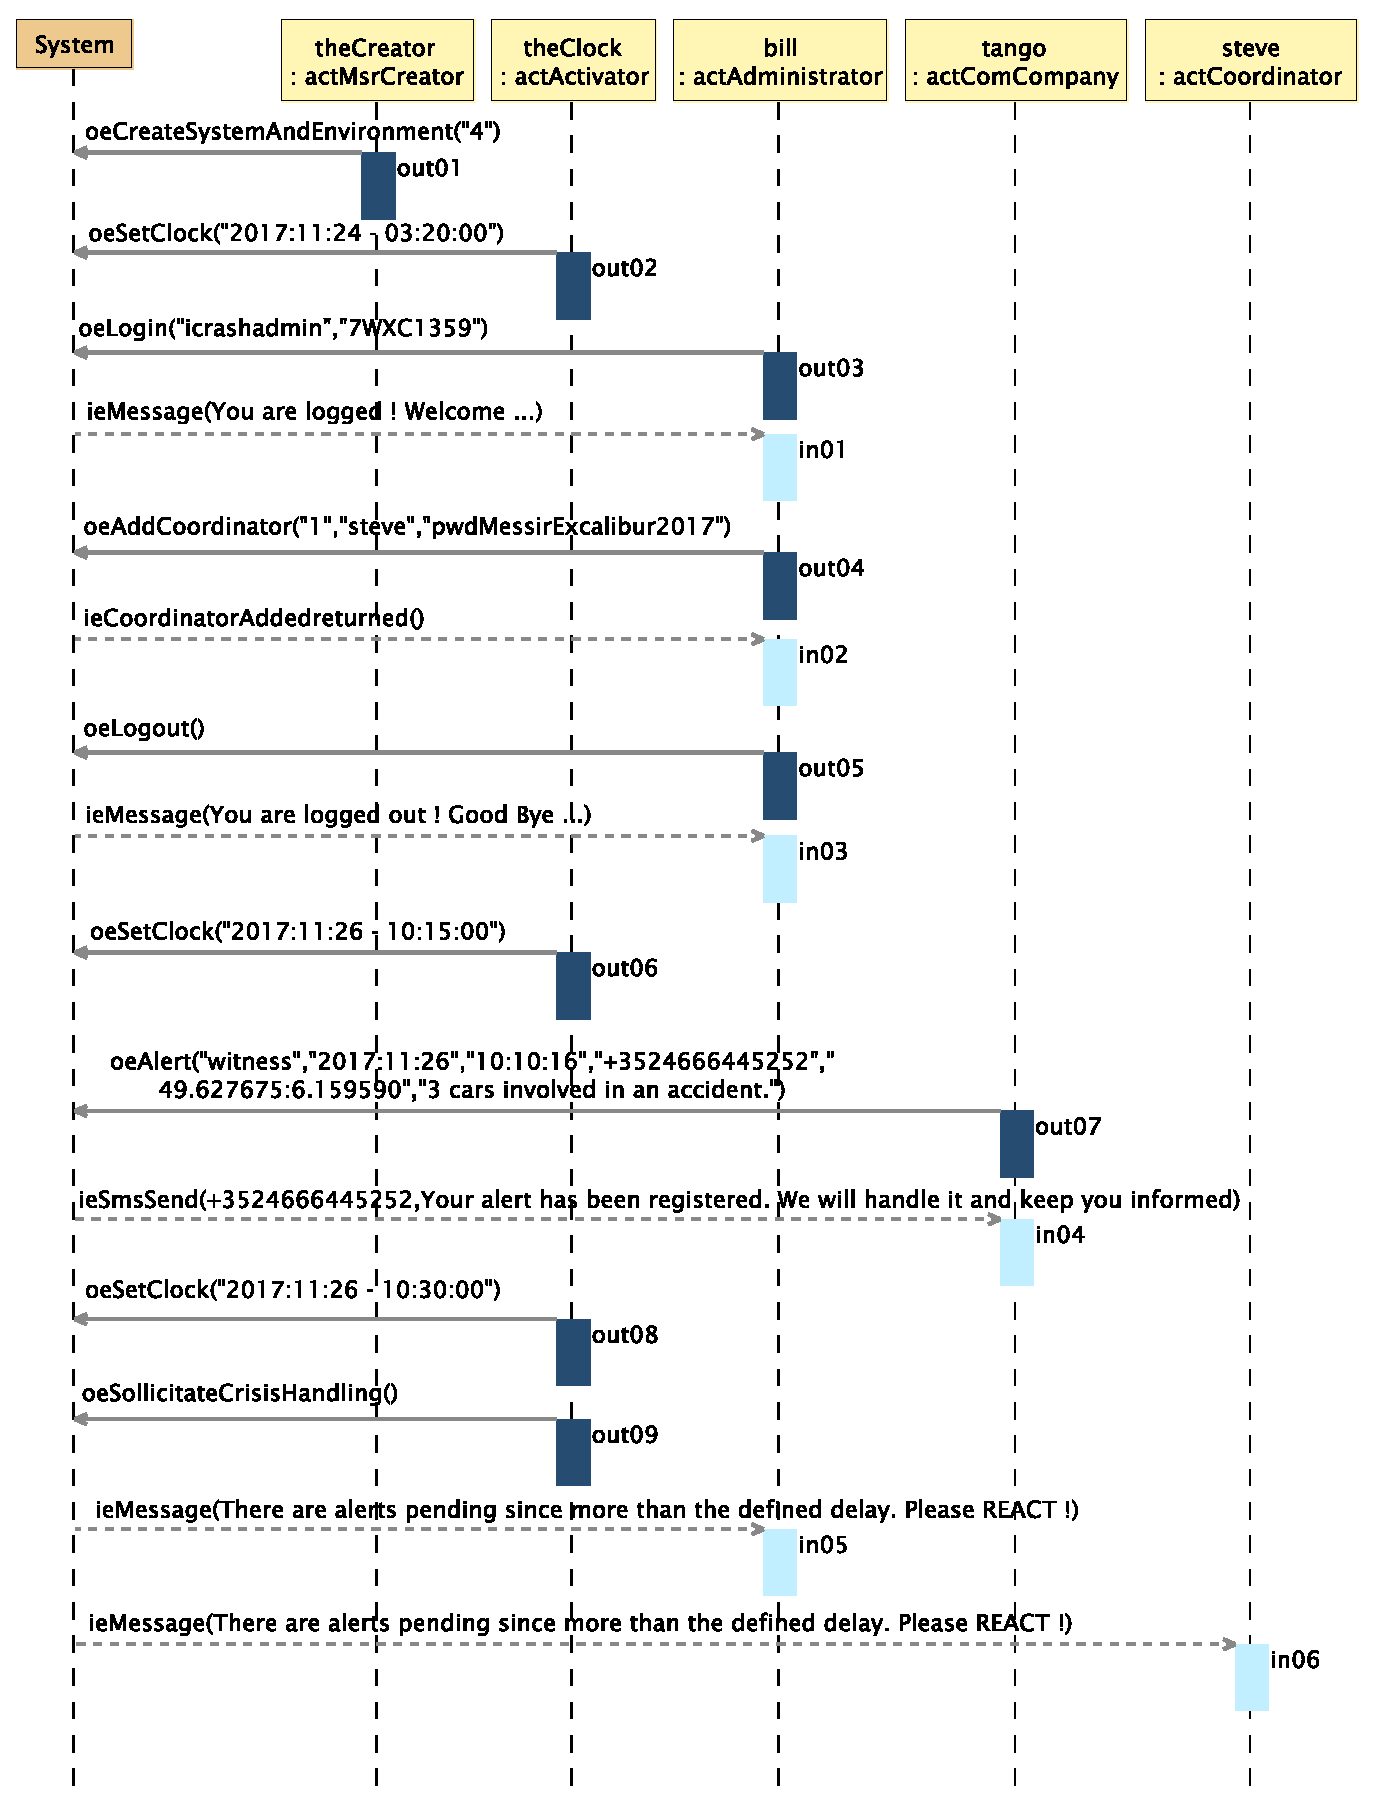
\includegraphics[
	angle=0
	,height=1.0\textheight
	]{./images-report-gen/usecase-model/summary/uci-suDeployAndRun-uciSimpleAndComplete-Part01.eps}
	\end{center}
	\caption[lu.uni.lassy.excalibur.examples.icrash Sequence Diagram: uci-suDeployAndRun-uciSimpleAndComplete-Part01]{uci-suDeployAndRun-uciSimpleAndComplete-Part01
	}
	\label{fig:lu.uni.lassy.excalibur.examples.icrash-RE-UC-uci-suDeployAndRun-uciSimpleAndComplete-Part01}
	\end{figure}
	\vspace{0.5cm}


	\subsubsection{Use-Case Instance - uciSimpleAndCompletePart02:suDeployAndRun}
	
	Second part of a simple and complete use case instance for the summary use case \msrcode{suDeployAndRun} illustrating a simple and complete interaction scenario primarily handled by an administrator in a concrete situation. 
	\begin{operationmodel}
	\addheading{summary Use-Case Instance}
	\adddoublerow{Instantiated Use Case}{suDeployAndRun}
	\adddoublerow{Instance ID}{uciSimpleAndCompletePart02}
	
	\addrowheading{Remarks}
	\addalphanumberedsinglerow{}{starts when the coordinator logs in the system until the full handling of all the existing crisis.}
	\addalphanumberedsinglerow{}{shows an instantiated case of handling of a crisis by a coordinator until its closure after reporting.}
	\end{operationmodel} 

	
	Figure \ref{fig:lu.uni.lassy.excalibur.examples.icrash-RE-UC-uci-suDeployAndRun-uciSimpleAndComplete-Part02}
	shows the sequence diagram representing the second part of a simple and complete use case instance for the summary use case \msrcode{suDeployAndRun}.
	
	\begin{figure}[htbp]
	\begin{center}
	
	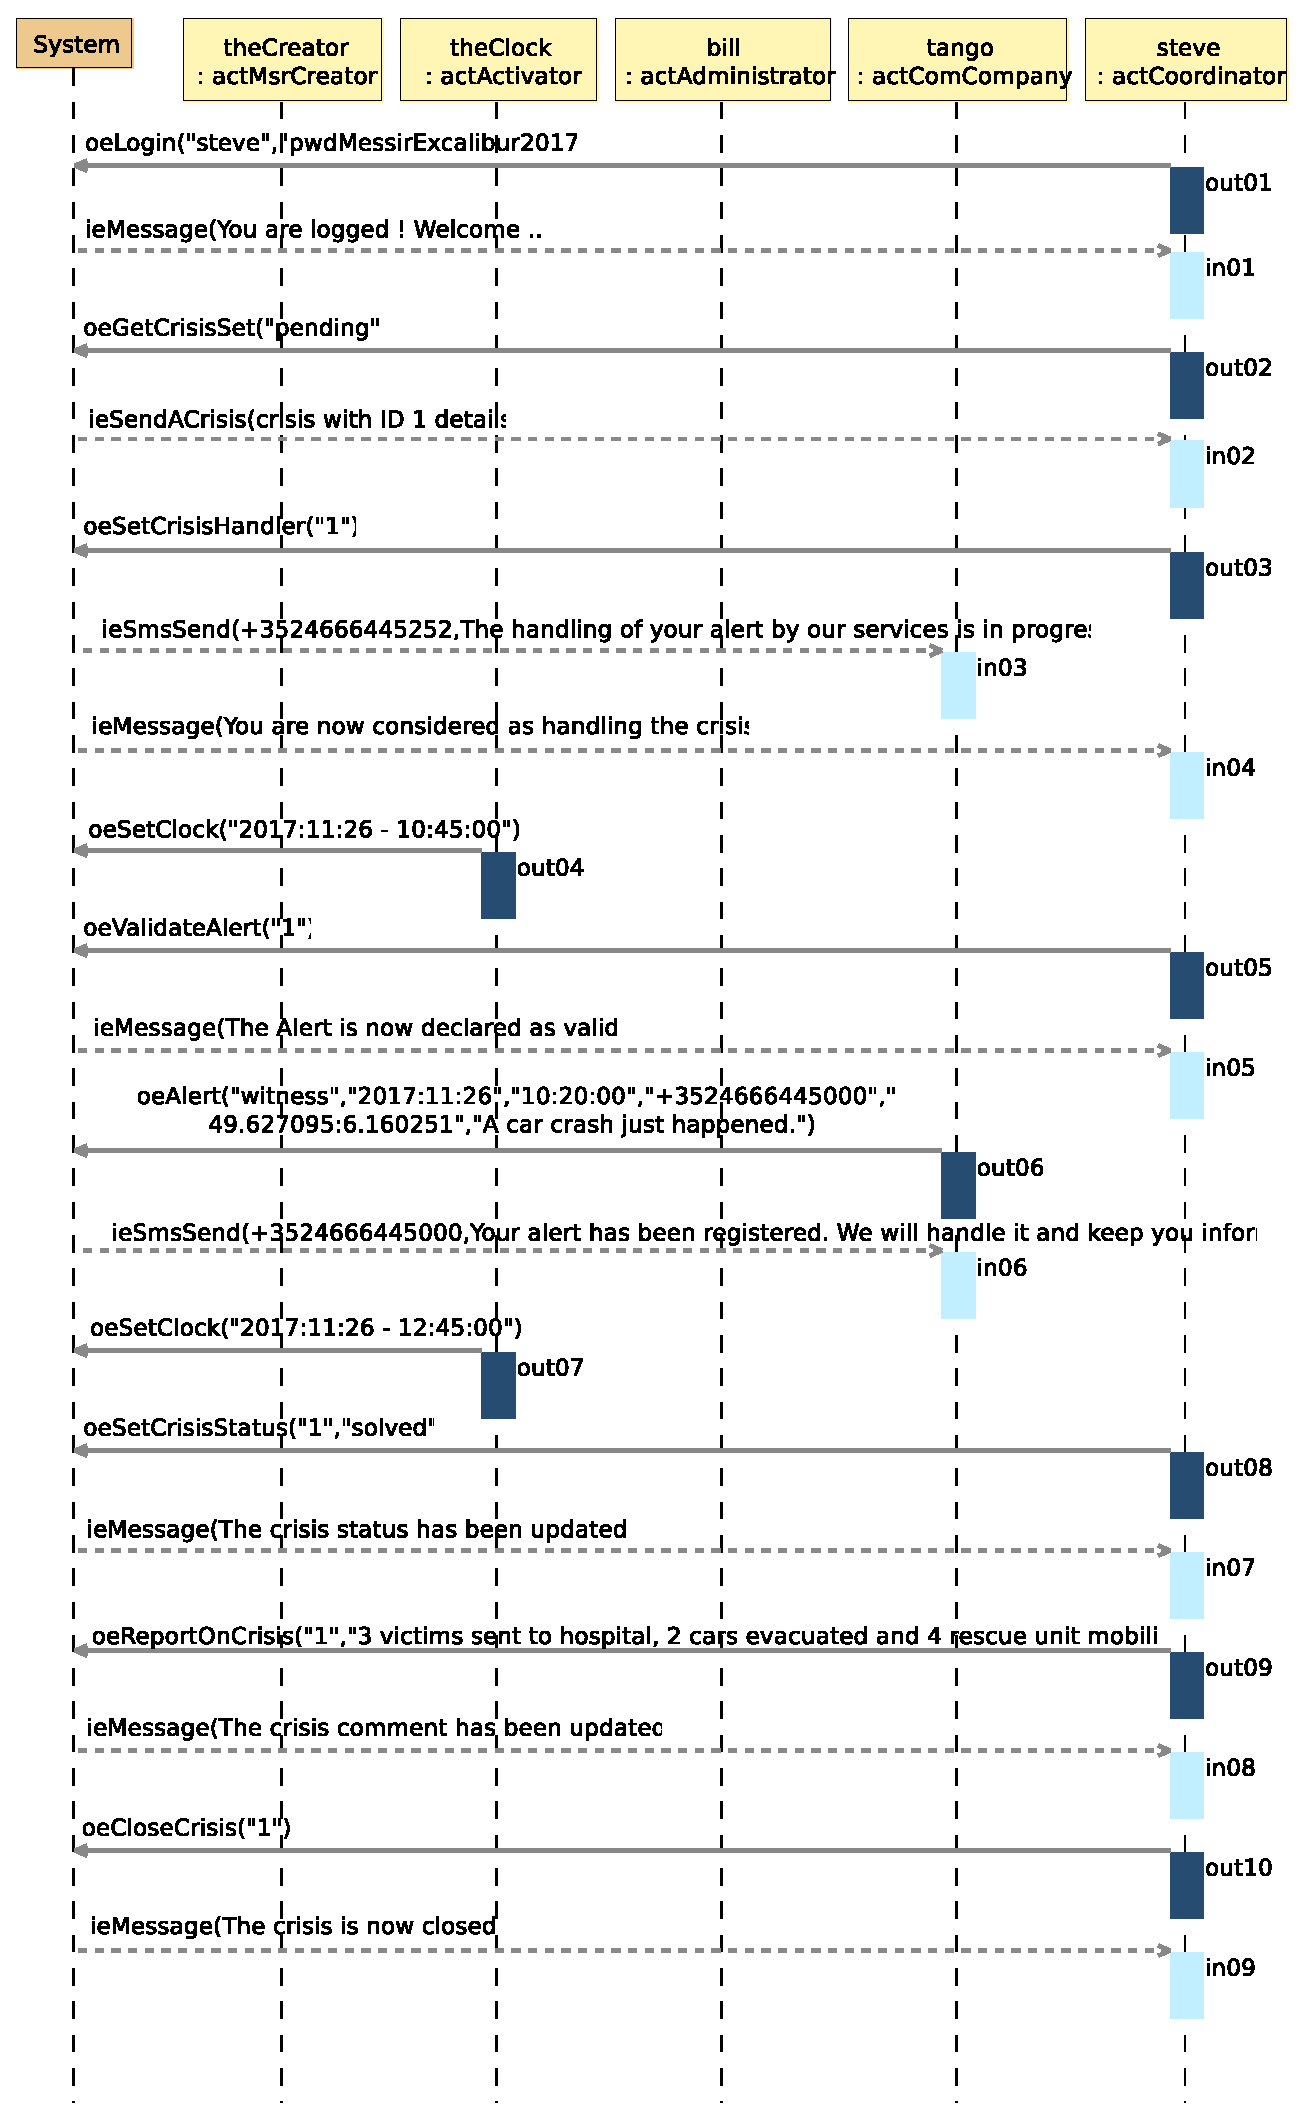
\includegraphics[
	angle=0
	,height=1.0\textheight
	]{./images-report-gen/usecase-model/summary/uci-suDeployAndRun-uciSimpleAndComplete-Part02.eps}
	\end{center}
	\caption[lu.uni.lassy.excalibur.examples.icrash Sequence Diagram: uci-suDeployAndRun-uciSimpleAndComplete-Part02]{uci-suDeployAndRun-uciSimpleAndComplete-Part02 use case instance sequence diagram
	}
	\label{fig:lu.uni.lassy.excalibur.examples.icrash-RE-UC-uci-suDeployAndRun-uciSimpleAndComplete-Part02}
	\end{figure}
	\vspace{0.5cm}




%% ***************************************************************
%% User-Goal Use Case Instances

	\subsubsection{Use-Case Instance - uciugSecurelyUseSystem:ugSecurelyUseSystem}
	
	\begin{operationmodel}
	\addheading{usergoal Use-Case Instance}
	\adddoublerow{Instantiated Use Case}{ugSecurelyUseSystem}
	\adddoublerow{Instance ID}{uciugSecurelyUseSystem}
	
	\end{operationmodel} 

	
	Figure \ref{fig:lu.uni.lassy.excalibur.examples.icrash-RE-UC-uci-uciugSecurelyUseSystem}
	
	\begin{figure}[htbp]
	\begin{center}
	
	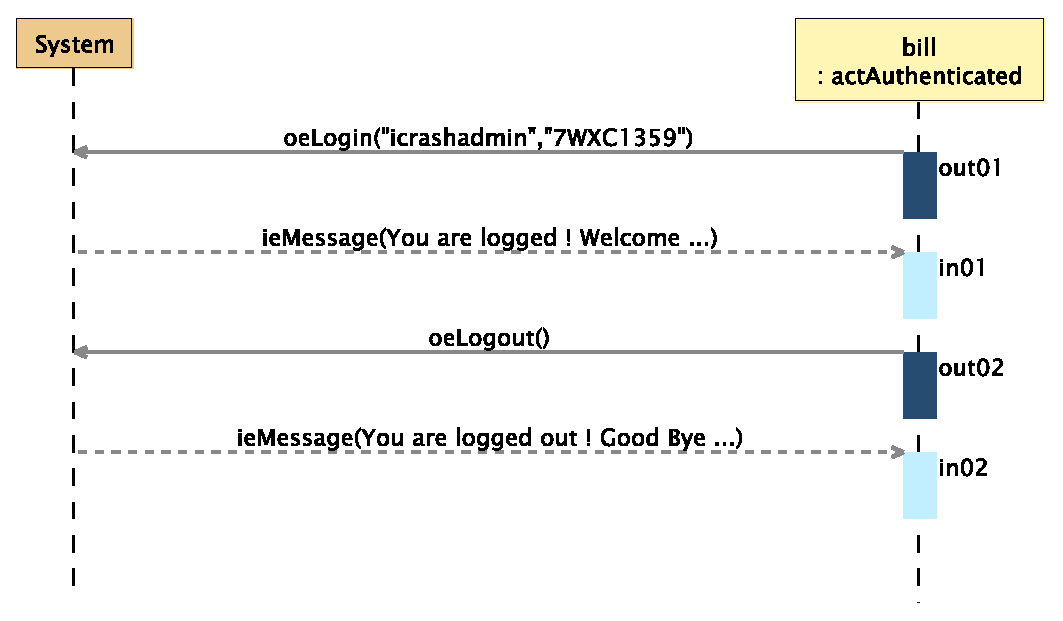
\includegraphics[
	angle=0
	]{./images-report-gen/usecase-model/usergoal/uci-uciugSecurelyUseSystem.eps}
	\end{center}
	\caption[lu.uni.lassy.excalibur.examples.icrash Sequence Diagram: uci-uciugSecurelyUseSystem]{}
	\label{fig:lu.uni.lassy.excalibur.examples.icrash-RE-UC-uci-uciugSecurelyUseSystem}
	\end{figure}
	\vspace{0.5cm}




%% ***************************************************************
%% Subfunction Use Case Instances


\chapter{Environment Model}
\label{chap:lu.uni.lassy.excalibur.examples.icrash-EM}



We provide below the view(s) defined for the \msrmessir environment model (cf. \cite{messirbook}) of the system. 


\section{Local view 01}
\label{sec:lu.uni.lassy.excalibur.examples.icrash-EM-view-01-local}

Figure \ref{fig:lu.uni.lassy.excalibur.examples.icrash-EM-view-local-01} 
shows the local view giving the second part of the environment model of the system in term of its state class, actors with their input and output interfaces and all related associations.


\begin{figure}[htbp] 
\label{fig:lu.uni.lassy.excalibur.examples.icrash-EM}
\begin{center}
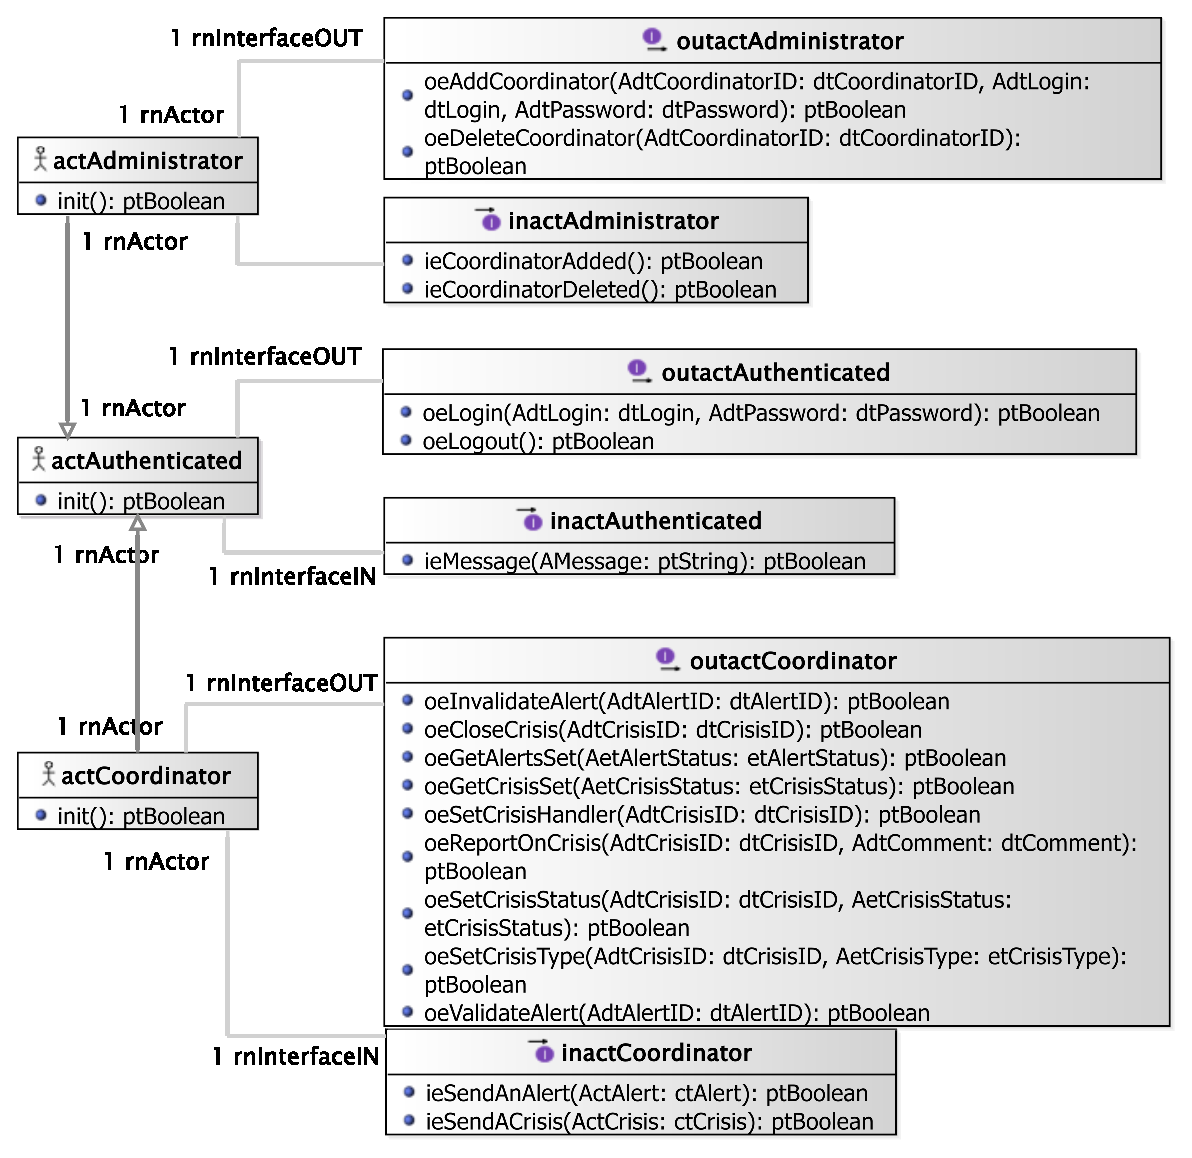
\includegraphics[
angle=0
,scale=0.80
]{./images-report-gen/environment-model/local/01/em-lv-01.eps}
\end{center}
\caption[Environment Model - Local View 01 - environment model local view - Part ]{Environment Model - Local View 01. environment model local view - Part 1.}
\label{fig:lu.uni.lassy.excalibur.examples.icrash-EM-view-local-01}
\end{figure}
\vspace{0.5cm} 

\section{Local view 02}
\label{sec:lu.uni.lassy.excalibur.examples.icrash-EM-view-02-local}

Figure \ref{fig:lu.uni.lassy.excalibur.examples.icrash-EM-view-local-02} 
shows the local view giving the second part the environment model of the system in term of its state class, actors with their input and output interfaces and all related associations.


\begin{figure}[htbp] 
\label{fig:lu.uni.lassy.excalibur.examples.icrash-EM}
\begin{center}
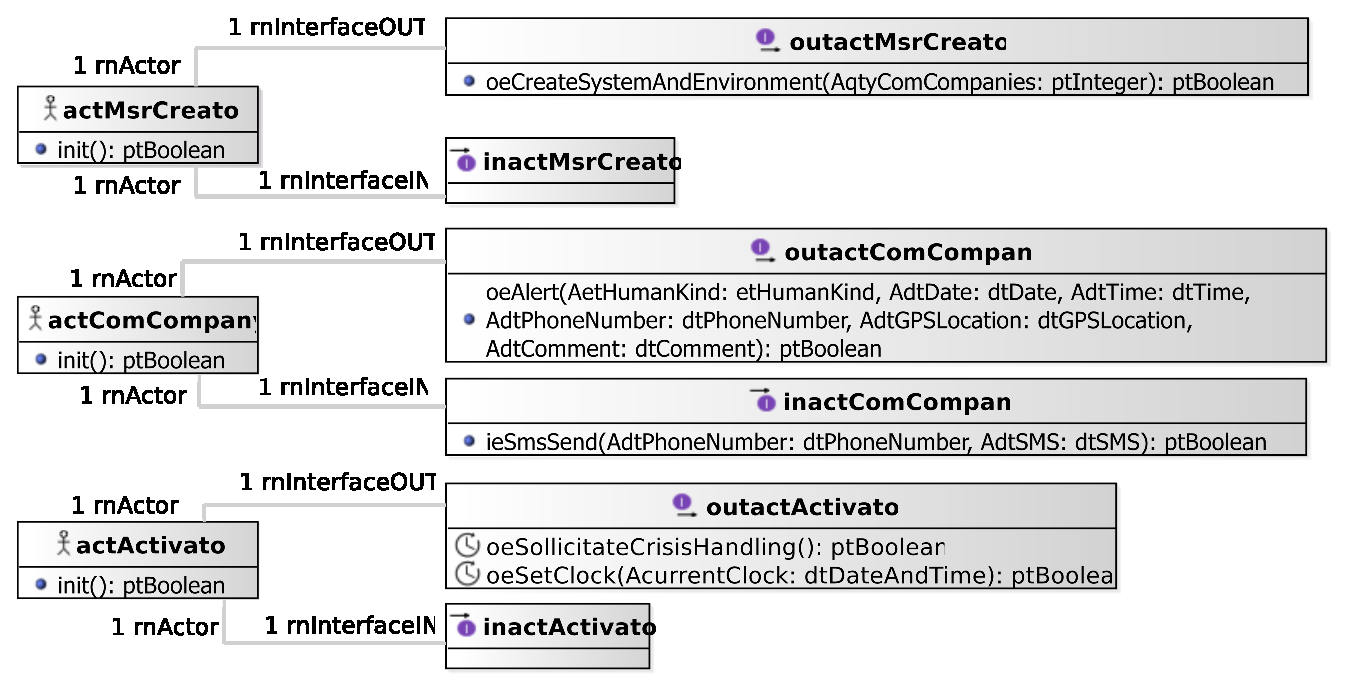
\includegraphics[
angle=0
,scale=0.80
]{./images-report-gen/environment-model/local/02/em-lv-02.eps}
\end{center}
\caption[Environment Model - Local View 02 - environment model local view - Part ]{Environment Model - Local View 02. environment model local view - Part 2.}
\label{fig:lu.uni.lassy.excalibur.examples.icrash-EM-view-local-02}
\end{figure}
\vspace{0.5cm} 

\section{Local view 03}
\label{sec:lu.uni.lassy.excalibur.examples.icrash-EM-view-03-local}

Figure \ref{fig:lu.uni.lassy.excalibur.examples.icrash-EM-view-local-03} shows the local view for the administrator actor and interfaces


\begin{figure}[htbp] 
\label{fig:lu.uni.lassy.excalibur.examples.icrash-EM}
\begin{center}
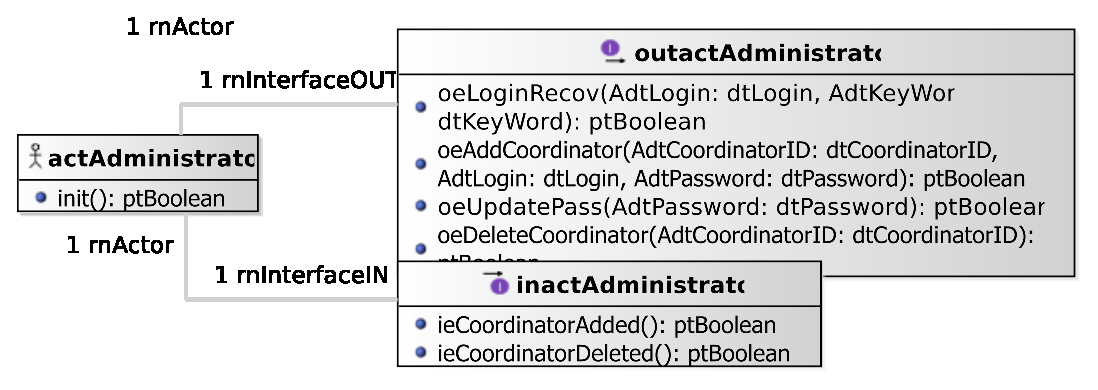
\includegraphics[
angle=0
,scale=0.80
]{./images-report-gen/environment-model/local/03/em-lv-03-parta-administrator.eps}
\end{center}
\caption[Environment Model - Local View 03 - administrator actor environment mode]{Environment Model - Local View 03. administrator actor environment model view.}
\label{fig:lu.uni.lassy.excalibur.examples.icrash-EM-view-local-03}
\end{figure}
\vspace{0.5cm} 

\section{Local view 04}
\label{sec:lu.uni.lassy.excalibur.examples.icrash-EM-view-04-local}

Figure \ref{fig:lu.uni.lassy.excalibur.examples.icrash-EM-view-local-04} shows the local view for the coordinator actor and interfaces


\begin{figure}[htbp] 
\label{fig:lu.uni.lassy.excalibur.examples.icrash-EM}
\begin{center}
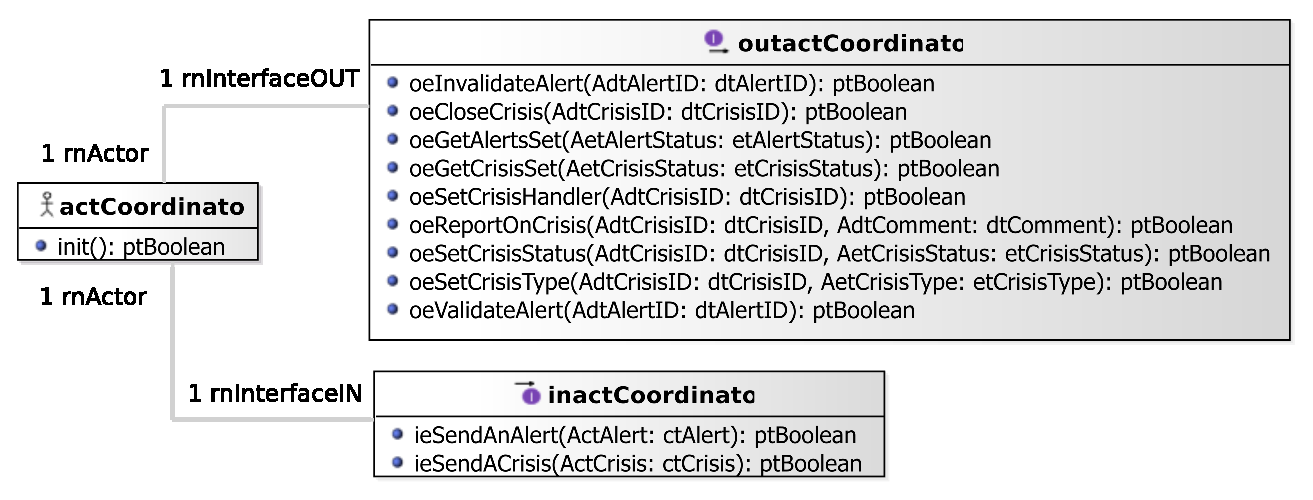
\includegraphics[
angle=0
,scale=0.80
]{./images-report-gen/environment-model/local/04/em-lv-04-partb-coordinator.eps}
\end{center}
\caption[Environment Model - Local View 04 - coordinator actor environment model ]{Environment Model - Local View 04. coordinator actor environment model view.}
\label{fig:lu.uni.lassy.excalibur.examples.icrash-EM-view-local-04}
\end{figure}
\vspace{0.5cm} 

\section{Local view 05}
\label{sec:lu.uni.lassy.excalibur.examples.icrash-EM-view-05-local}

Figure \ref{fig:lu.uni.lassy.excalibur.examples.icrash-EM-view-local-05} shows the local view for the authenticated actor and interfaces


\begin{figure}[htbp] 
\label{fig:lu.uni.lassy.excalibur.examples.icrash-EM}
\begin{center}
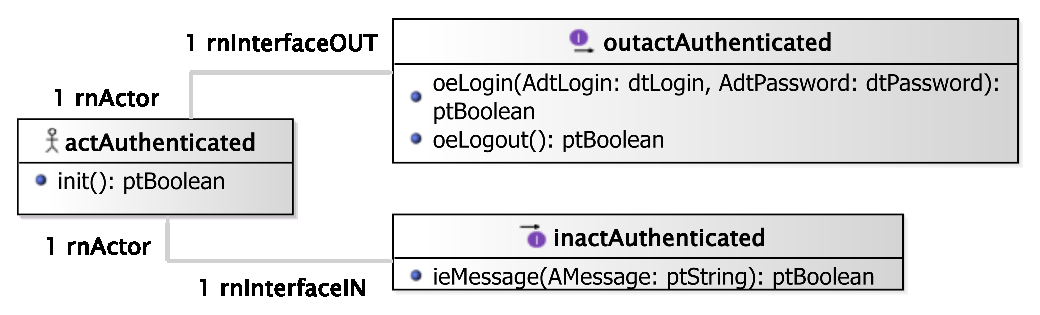
\includegraphics[
angle=0
,scale=0.80
]{./images-report-gen/environment-model/local/05/em-lv-05-partc-authenticated.eps}
\end{center}
\caption[Environment Model - Local View 05 - authenticated actor environment mode]{Environment Model - Local View 05. authenticated actor environment model local view.}
\label{fig:lu.uni.lassy.excalibur.examples.icrash-EM-view-local-05}
\end{figure}
\vspace{0.5cm} 



\section{Global view 01}
\label{sec:lu.uni.lassy.excalibur.examples.icrash-EM-view-01-global}
\clearpage

Figure \ref{fig:lu.uni.lassy.excalibur.examples.icrash-EM-view-global-01} shows a global view for all actors with their relationships with ctState


\begin{figure}[htbp] 
\label{fig:lu.uni.lassy.excalibur.examples.icrash-EM}
\begin{center}
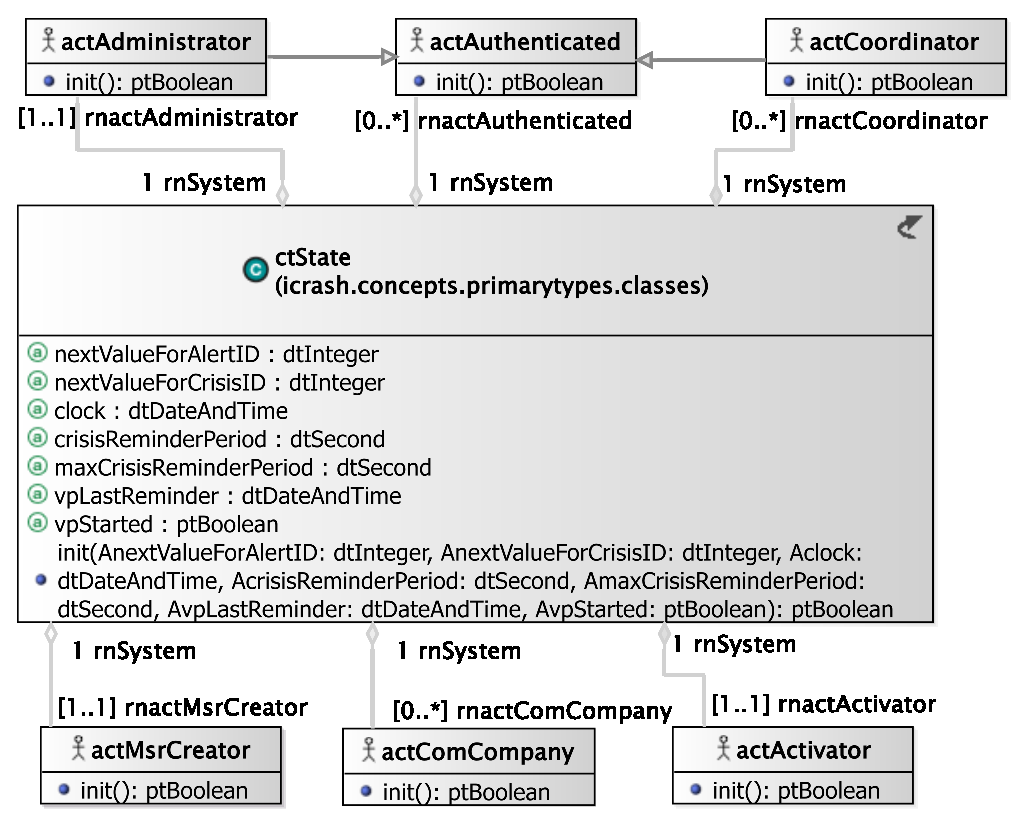
\includegraphics[
angle=0
,scale=0.80
]{./images-report-gen/environment-model/global/01/em-gv-01.eps}
\end{center}
\caption[Environment Model - Global View 01 -  em-gv-01 environment model global v]{Environment Model - Global View 01.  em-gv-01 environment model global view.}
\label{fig:lu.uni.lassy.excalibur.examples.icrash-EM-view-global-01}
\end{figure}
\vspace{0.5cm} 




\section{Actors and Interfaces Descriptions}
\label{sec:lu.uni.lassy.excalibur.examples.icrash-EM-Actors-Descriptions}


		
We provide for the given views the description of the actors together with their associated input and output interface descriptions.
\subsection{\msrcode{actActivator} Actor}


\begin{actortable}
	\addheading{Actor}
	
	\adddoublerow{actActivator}{represents a logical actor for time automatic message sending based on system's or environment status.}
	
	
	
	
	

	\addrowheading{OutputInterfaces}
	\addnumbereddoublerow{OUT}{\hypertarget{actActivator.outactActivator.oeSollicitateCrisisHandling}
			{\msrcode{[proactive] oeSollicitateCrisisHandling():ptBoolean}}}
			{used to avoid crisis to stay too long in an not handled status.}
	\addnumbereddoublerow{OUT}{\hypertarget{actActivator.outactActivator.oeSetClock}
			{\msrcode{[proactive] oeSetClock(AcurrentClock:dtDateAndTime):ptBoolean}}}
			{used to update the system's time}
	
	
\end{actortable}

\subsection{\msrcode{actAdministrator} Actor}


\begin{actortable}
	\addheading{Actor}
	
	\adddoublerow{actAdministrator}{represents an actor responsible of administration tasks for the \msricrash system.}
	
	\addrowheading{Extends}
	\addsinglerow{icrash.environment.actAuthenticated}
	
	
	
	
	

	\addrowheading{OutputInterfaces}
	\addnumbereddoublerow{OUT}{\hypertarget{actAdministrator.outactAdministrator.oeAddCoordinator}
			{\msrcode{oeAddCoordinator(AdtCoordinatorID:dtCoordinatorID, AdtLogin:dtLogin, AdtPassword:dtPassword):ptBoolean}}}
			{sent to add a new coordinator in the system's post state and environment's post state.}
	\addnumbereddoublerow{OUT}{\hypertarget{actAdministrator.outactAdministrator.oeDeleteCoordinator}
			{\msrcode{oeDeleteCoordinator(AdtCoordinatorID:dtCoordinatorID):ptBoolean}}}
			{sent to delete an existing coordinator in the system's post state and environment's post state.}
	
	\addrowheading{InputInterfaces}
	\addnumbereddoublerow{IN}{\msrcode{ieCoordinatorAdded():ptBoolean}}
							 {its reception confirms the creation of the requested coodinator. }
	\addnumbereddoublerow{IN}{\msrcode{ieCoordinatorDeleted():ptBoolean}}
							 {its reception confirms the deletion of the requested coodinator. }
	
\end{actortable}

\subsection{\msrcode{actAuthenticated} Actor}


\begin{actortable}
	\addheading{Actor}
	
	\adddoublerow{actAuthenticated}{abstract actor providing reusable input and output interfaces for actors that need to authenticate themselves.}
	
	
	
	
	

	\addrowheading{OutputInterfaces}
	\addnumbereddoublerow{OUT}{\hypertarget{actAuthenticated.outactAuthenticated.oeLogin}
			{\msrcode{oeLogin(AdtLogin:dtLogin, AdtPassword:dtPassword):ptBoolean}}}
			{sent to request authorization to request access secured system operations.}
	\addnumbereddoublerow{OUT}{\hypertarget{actAuthenticated.outactAuthenticated.oeLogout}
			{\msrcode{oeLogout():ptBoolean}}}
			{sent to end the secured access to specific system operations.}
	
	\addrowheading{InputInterfaces}
	\addnumbereddoublerow{IN}{\msrcode{ieMessage(AMessage:ptString):ptBoolean}}
							 {allows for receiving general textual messages.}
	
\end{actortable}

\subsection{\msrcode{actComCompany} Actor}


\begin{actortable}
	\addheading{Actor}
	
	\adddoublerow{actComCompany}{represents the communication company stakeholder ensuring the input/ouput of textual messages with humans having communicaiton devices.}
	
	
	
	
	

	\addrowheading{OutputInterfaces}
	\addnumbereddoublerow{OUT}{\hypertarget{actComCompany.outactComCompany.oeAlert}
			{\msrcode{oeAlert(AetHumanKind:etHumanKind, AdtDate:dtDate, AdtTime:dtTime, AdtPhoneNumber:dtPhoneNumber, AdtGPSLocation:dtGPSLocation, AdtComment:dtComment, ADeadline:dtDateAndTime):ptBoolean}}}
			{sent to alert of a potential crisis situation.}
	
	\addrowheading{InputInterfaces}
	\addnumbereddoublerow{IN}{\msrcode{ieSmsSend(AdtPhoneNumber:dtPhoneNumber, AdtSMS:dtSMS):ptBoolean}}
							 {allows for receiving textual messages to be dispatched to the communication company customers having the provided phone number.}
	
\end{actortable}

\subsection{\msrcode{actCoordinator} Actor}


\begin{actortable}
	\addheading{Actor}
	
	\adddoublerow{actCoordinator}{represents actor responsible of handling one or several crisis for the \msricrash system.}
	
	\addrowheading{Extends}
	\addsinglerow{icrash.environment.actAuthenticated}
	
	
	
	
	

	\addrowheading{OutputInterfaces}
	\addnumbereddoublerow{OUT}{\hypertarget{actCoordinator.outactCoordinator.oeInvalidateAlert}
			{\msrcode{oeInvalidateAlert(AdtAlertID:dtAlertID):ptBoolean}}}
			{sent to indicate that an alert should be considered as closed.}
	\addnumbereddoublerow{OUT}{\hypertarget{actCoordinator.outactCoordinator.oeCloseCrisis}
			{\msrcode{oeCloseCrisis(AdtCrisisID:dtCrisisID):ptBoolean}}}
			{sent to indicate that a crisis should be considered as closed.}
	\addnumbereddoublerow{OUT}{\hypertarget{actCoordinator.outactCoordinator.oeGetAlertsSet}
			{\msrcode{oeGetAlertsSet(AetAlertStatus:etAlertStatus):ptBoolean}}}
			{sent to request all the ctAlert instances having a specific status.}
	\addnumbereddoublerow{OUT}{\hypertarget{actCoordinator.outactCoordinator.oeGetCrisisSet}
			{\msrcode{oeGetCrisisSet(AetCrisisStatus:etCrisisStatus):ptBoolean}}}
			{sent to request all the ctCrisis instances having a specific status.}
	\addnumbereddoublerow{OUT}{\hypertarget{actCoordinator.outactCoordinator.oeSetCrisisHandler}
			{\msrcode{oeSetCrisisHandler(AdtCrisisID:dtCrisisID):ptBoolean}}}
			{sent to declare himself as been the handler of a crisis having the specified id.}
	\addnumbereddoublerow{OUT}{\hypertarget{actCoordinator.outactCoordinator.oeReportOnCrisis}
			{\msrcode{oeReportOnCrisis(AdtCrisisID:dtCrisisID, AdtComment:dtComment):ptBoolean}}}
			{sent to update the textual information available for a specific handled crisis.}
	\addnumbereddoublerow{OUT}{\hypertarget{actCoordinator.outactCoordinator.oeSetCrisisStatus}
			{\msrcode{oeSetCrisisStatus(AdtCrisisID:dtCrisisID, AetCrisisStatus:etCrisisStatus):ptBoolean}}}
			{sent to define the handling status of a specific crisis.}
	\addnumbereddoublerow{OUT}{\hypertarget{actCoordinator.outactCoordinator.oeSetCrisisType}
			{\msrcode{oeSetCrisisType(AdtCrisisID:dtCrisisID, AetCrisisType:etCrisisType):ptBoolean}}}
			{sent to define the gravity type of a specific crisis.}
	\addnumbereddoublerow{OUT}{\hypertarget{actCoordinator.outactCoordinator.oeValidateAlert}
			{\msrcode{oeValidateAlert(AdtAlertID:dtAlertID):ptBoolean}}}
			{sent to indicate that a specific alert is not a fake.}
	
	\addrowheading{InputInterfaces}
	\addnumbereddoublerow{IN}{\msrcode{ieSendAnAlert(ActAlert:ctAlert):ptBoolean}}
							 {allows for receiving a requested ctAlert instance.}
	\addnumbereddoublerow{IN}{\msrcode{ieSendACrisis(ActCrisis:ctCrisis):ptBoolean}}
							 {allows for receiving a requested ctCrisis instance.}
	
\end{actortable}

\subsection{\msrcode{actMsrCreator} Actor}


\begin{actortable}
	\addheading{Actor}
	
	\adddoublerow{actMsrCreator}{Represents the creator stakeholder in charge of state and environment initialization.}
	
	
	
	
	

	\addrowheading{OutputInterfaces}
	\addnumbereddoublerow{OUT}{\hypertarget{actMsrCreator.outactMsrCreator.oeCreateSystemAndEnvironment}
			{\msrcode{oeCreateSystemAndEnvironment(AqtyComCompanies:ptInteger):ptBoolean}}}
			{sent to request the initialization of the system's class instances and the environment actors instances.}
	
	
\end{actortable}




\chapter{Concept Model}
\label{chap:lu.uni.lassy.excalibur.examples.icrash-CM}


\section{PrimaryTypes-Classes}
\subsection{Local view 01}
\label{sec:lu.uni.lassy.excalibur.examples.icrash-CM-view-local-PrimaryTypes-Classes-01}
Figure \ref{fig:lu.uni.lassy.excalibur.examples.icrash-CM-view-local-PrimaryTypes-Classes-01} 
shows the local view on all the primary types class types.



\begin{figure}[htbp] 
\label{fig:lu.uni.lassy.excalibur.examples.icrash-CM}
\begin{center}
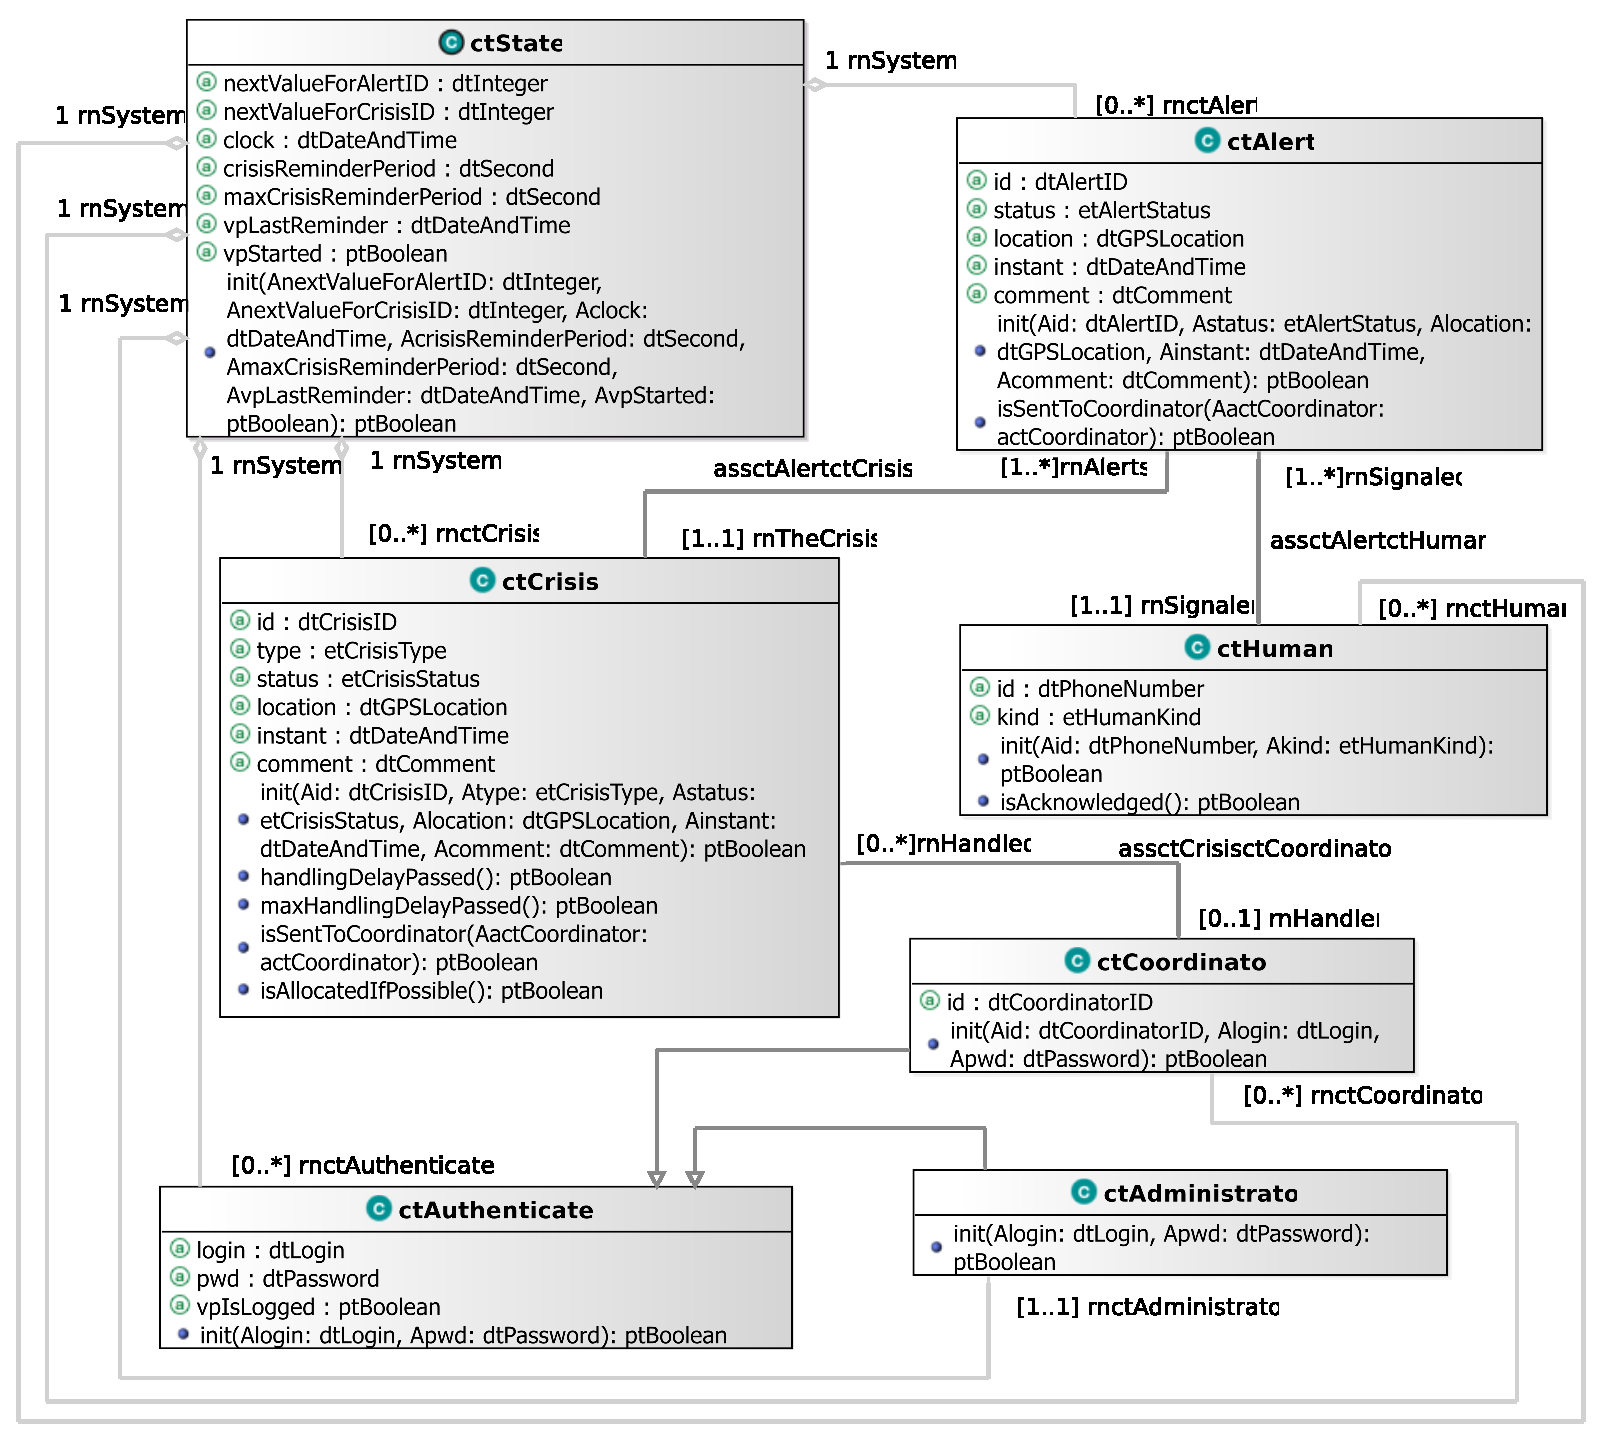
\includegraphics[
angle=0
,width=1.0\textwidth
]{./images-report-gen/concept-model/local/PrimaryTypes-Classes/01/cm-pt-ct-lv-01.eps}
\end{center}
\caption[Concept Model - PrimaryTypes-Classes local view 01 - Local view of all the primary types ]{Concept Model - PrimaryTypes-Classes local view 01. Local view of all the primary types class types
.}
\label{fig:lu.uni.lassy.excalibur.examples.icrash-CM-view-local-PrimaryTypes-Classes-01}
\end{figure}
\vspace{0.5cm} 

\subsection{Local view 02}
\label{sec:lu.uni.lassy.excalibur.examples.icrash-CM-view-local-PrimaryTypes-Classes-02}
Figure \ref{fig:lu.uni.lassy.excalibur.examples.icrash-CM-view-local-PrimaryTypes-Classes-02} shows the local view of the ctState primary type class type.



\begin{figure}[htbp] 
\label{fig:lu.uni.lassy.excalibur.examples.icrash-CM}
\begin{center}
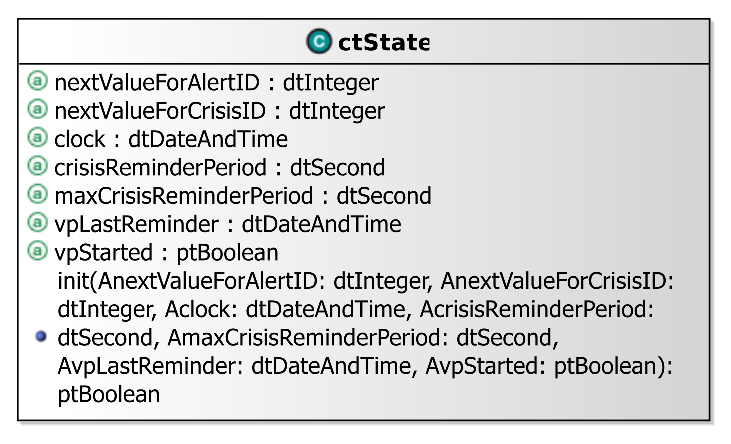
\includegraphics[
angle=0
,scale=0.80
]{./images-report-gen/concept-model/local/PrimaryTypes-Classes/02/cm-pt-ct-lv-02-parta-ctState.eps}
\end{center}
\caption[Concept Model - PrimaryTypes-Classes local view 02 - local view of the ctState primary ty]{Concept Model - PrimaryTypes-Classes local view 02. local view of the ctState primary type.}
\label{fig:lu.uni.lassy.excalibur.examples.icrash-CM-view-local-PrimaryTypes-Classes-02}
\end{figure}
\vspace{0.5cm} 

\subsection{Local view 03}
\label{sec:lu.uni.lassy.excalibur.examples.icrash-CM-view-local-PrimaryTypes-Classes-03}
Figure \ref{fig:lu.uni.lassy.excalibur.examples.icrash-CM-view-local-PrimaryTypes-Classes-03} shows the local view of the ctAlert primary type class type.



\begin{figure}[htbp] 
\label{fig:lu.uni.lassy.excalibur.examples.icrash-CM}
\begin{center}
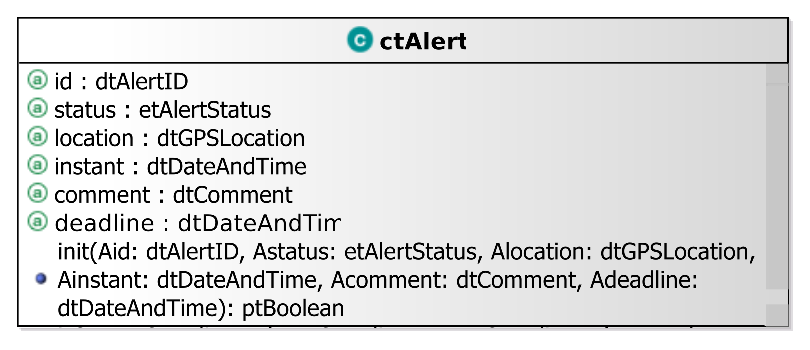
\includegraphics[
angle=0
,scale=0.80
]{./images-report-gen/concept-model/local/PrimaryTypes-Classes/03/cm-pt-ct-lv-03-partb-ctAlert.eps}
\end{center}
\caption[Concept Model - PrimaryTypes-Classes local view 03 - local view of the ctAlert primary ty]{Concept Model - PrimaryTypes-Classes local view 03. local view of the ctAlert primary type.}
\label{fig:lu.uni.lassy.excalibur.examples.icrash-CM-view-local-PrimaryTypes-Classes-03}
\end{figure}
\vspace{0.5cm} 

\subsection{Local view 04}
\label{sec:lu.uni.lassy.excalibur.examples.icrash-CM-view-local-PrimaryTypes-Classes-04}
Figure \ref{fig:lu.uni.lassy.excalibur.examples.icrash-CM-view-local-PrimaryTypes-Classes-04} shows the local view of the ctCrisis primary type class type.



\begin{figure}[htbp] 
\label{fig:lu.uni.lassy.excalibur.examples.icrash-CM}
\begin{center}
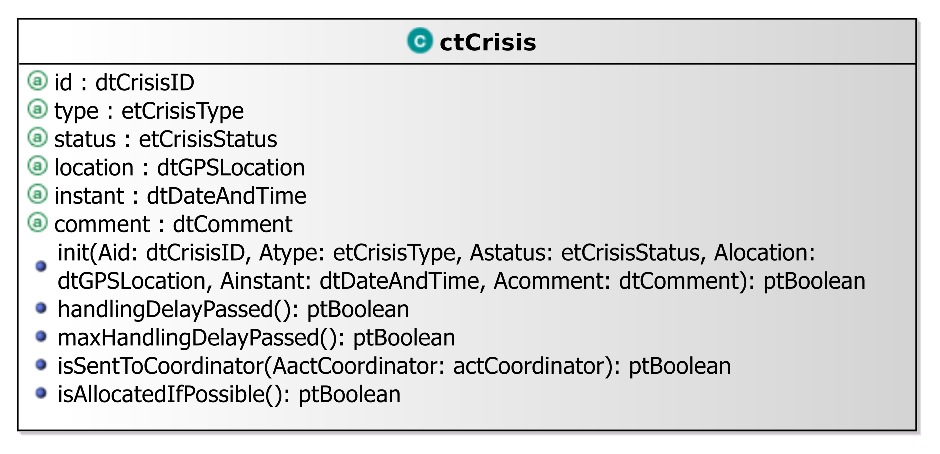
\includegraphics[
angle=0
,scale=0.80
]{./images-report-gen/concept-model/local/PrimaryTypes-Classes/04/cm-pt-ct-lv-04-partc-ctCrisis.eps}
\end{center}
\caption[Concept Model - PrimaryTypes-Classes local view 04 - local view of the ctCrisis primary t]{Concept Model - PrimaryTypes-Classes local view 04. local view of the ctCrisis primary type.}
\label{fig:lu.uni.lassy.excalibur.examples.icrash-CM-view-local-PrimaryTypes-Classes-04}
\end{figure}
\vspace{0.5cm} 


\subsection{Global view 01}
\label{sec:lu.uni.lassy.excalibur.examples.icrash-CM-view-global-PrimaryTypes-Classes-01}
Figure \ref{fig:lu.uni.lassy.excalibur.examples.icrash-CM-view-global-PrimaryTypes-Classes-01} 
shows the global view on primary types class types showing the association(s) types with the actor classes of the environment model.



\begin{figure}[htbp] 
\label{fig:lu.uni.lassy.excalibur.examples.icrash-CM}
\begin{center}
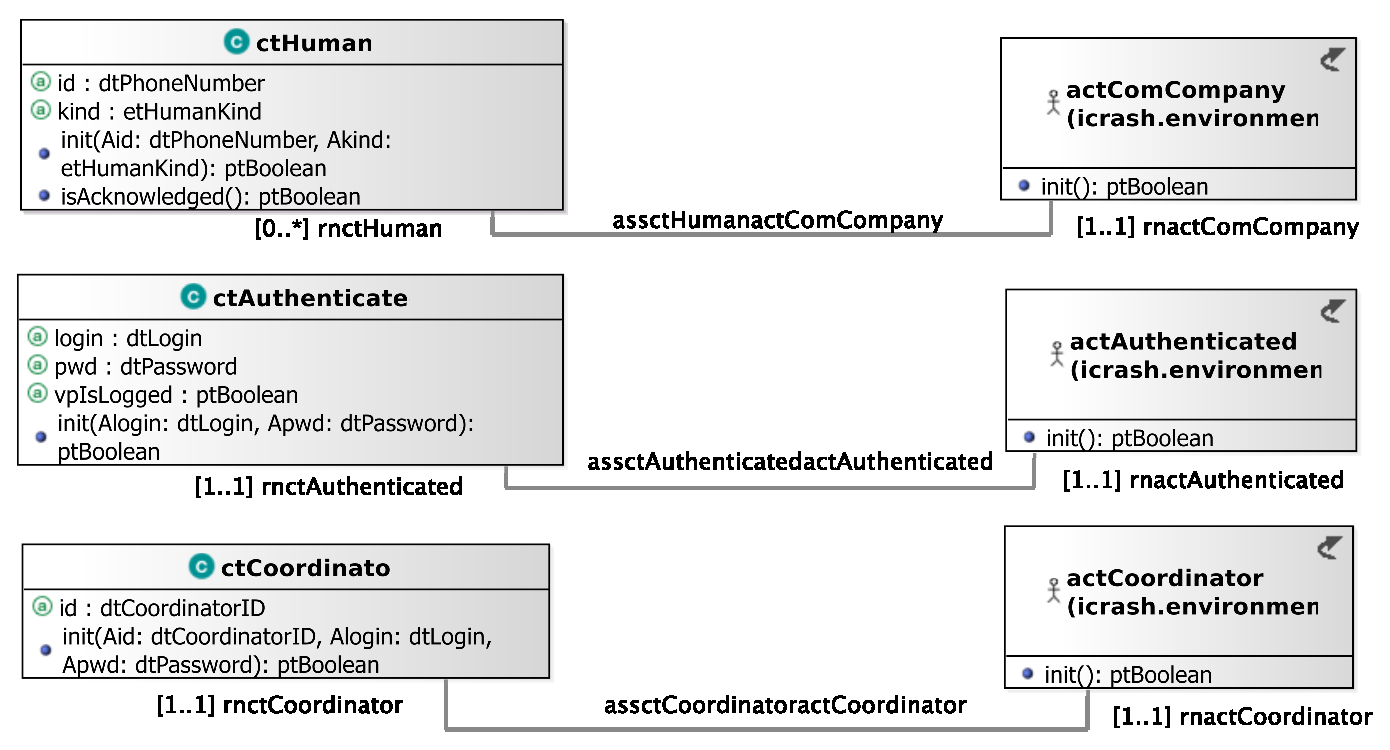
\includegraphics[
angle=0
,width=1.0\textwidth
]{./images-report-gen/concept-model/global/PrimaryTypes-Classes/01/cm-pt-ct-gv-01.eps}
\end{center}
\caption[Concept Model - PrimaryTypes-Classes global view 01 -  Primary types class types global vi]{Concept Model - PrimaryTypes-Classes global view 01.  Primary types class types global view - cm-pt-ct-gv-01
.}
\label{fig:lu.uni.lassy.excalibur.examples.icrash-CM-view-global-PrimaryTypes-Classes-01}
\end{figure}
\vspace{0.5cm} 



\section{PrimaryTypes-Datatypes}
\subsection{Local view 06}
\label{sec:lu.uni.lassy.excalibur.examples.icrash-CM-view-local-PrimaryTypes-Datatypes-06}
Figure \ref{fig:lu.uni.lassy.excalibur.examples.icrash-CM-view-local-PrimaryTypes-Datatypes-06} 



\begin{figure}[htbp] 
\label{fig:lu.uni.lassy.excalibur.examples.icrash-CM}
\begin{center}
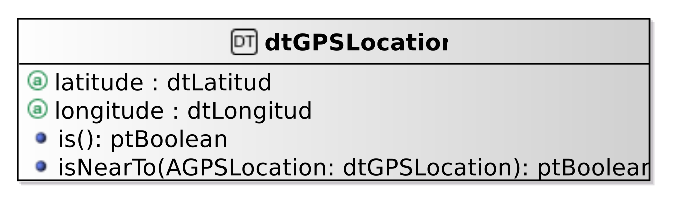
\includegraphics[
angle=0
]{./images-report-gen/concept-model/local/PrimaryTypes-Datatypes/06/cm-pt-dt-lv-02-dtGPSLocation.eps}
\end{center}
\caption[Concept Model - PrimaryTypes-Datatypes local view 06 - ]{Concept Model - PrimaryTypes-Datatypes local view 06. .}
\label{fig:lu.uni.lassy.excalibur.examples.icrash-CM-view-local-PrimaryTypes-Datatypes-06}
\end{figure}
\vspace{0.5cm} 


\subsection{Global view 01}
\label{sec:lu.uni.lassy.excalibur.examples.icrash-CM-view-global-PrimaryTypes-Datatypes-01}
Figure \ref{fig:lu.uni.lassy.excalibur.examples.icrash-CM-view-global-PrimaryTypes-Datatypes-01} 
shows a global view on the \msricrash primary types datatype types.



\begin{figure}[htbp] 
\label{fig:lu.uni.lassy.excalibur.examples.icrash-CM}
\begin{center}
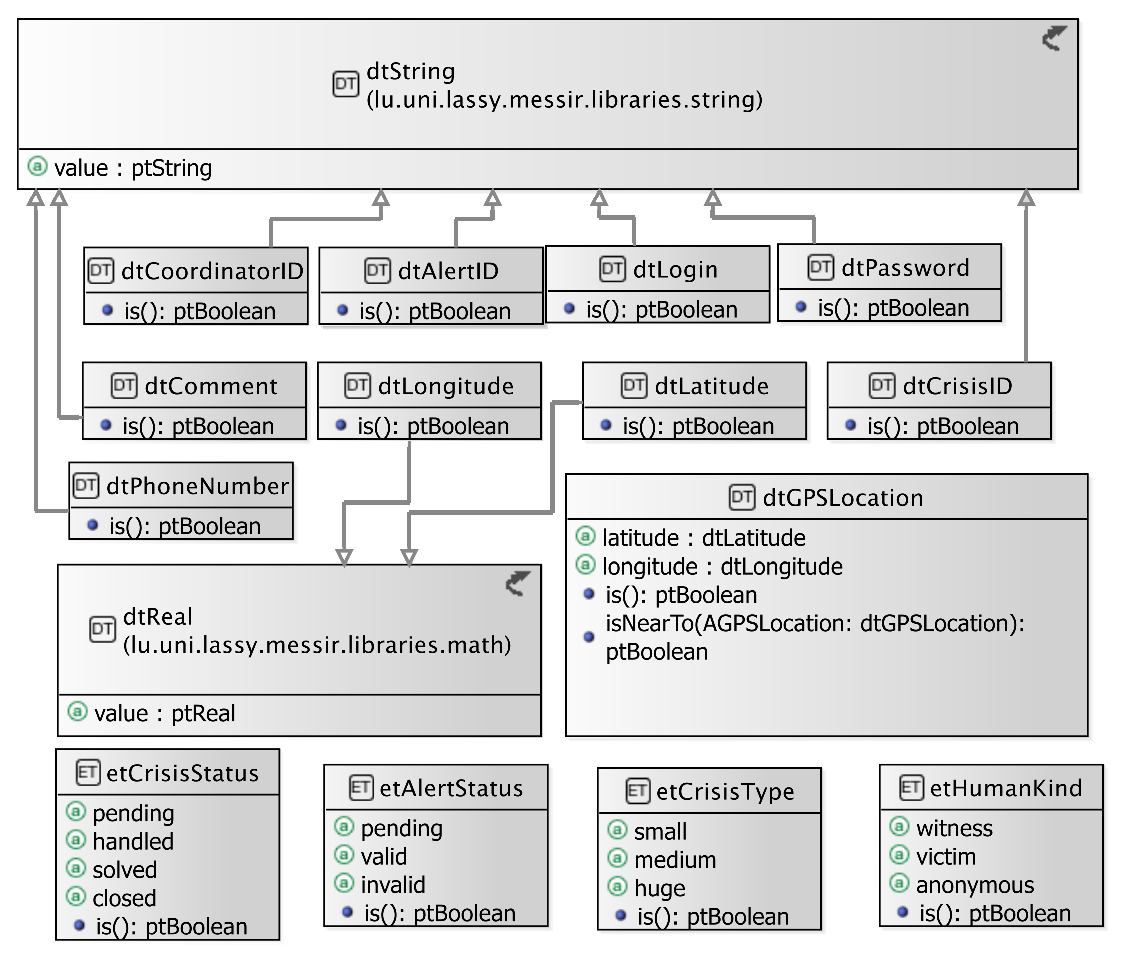
\includegraphics[
angle=0
,width=1.0\textwidth
]{./images-report-gen/concept-model/global/PrimaryTypes-Datatypes/01/cm-pt-dt-gv-01.eps}
\end{center}
\caption[Concept Model - PrimaryTypes-Datatypes global view 01 -  global view of primary types dataty]{Concept Model - PrimaryTypes-Datatypes global view 01.  global view of primary types datatype types - cm-pt-dt-gv-01
.}
\label{fig:lu.uni.lassy.excalibur.examples.icrash-CM-view-global-PrimaryTypes-Datatypes-01}
\end{figure}
\vspace{0.5cm} 





\section{SecondaryTypes-Datatypes}
\subsection{Local view 01}
\label{sec:lu.uni.lassy.excalibur.examples.icrash-CM-view-local-SecondaryTypes-Datatypes-01}
Figure \ref{fig:lu.uni.lassy.excalibur.examples.icrash-CM-view-local-SecondaryTypes-Datatypes-01} shows the local view of the secondary types datatype types.



\begin{figure}[htbp] 
\label{fig:lu.uni.lassy.excalibur.examples.icrash-CM}
\begin{center}
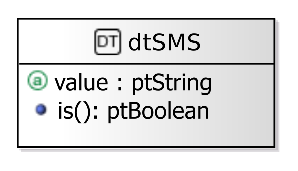
\includegraphics[
angle=0
]{./images-report-gen/concept-model/local/SecondaryTypes-Datatypes/01/cm-st-dt-lv-01.eps}
\end{center}
\caption[Concept Model - SecondaryTypes-Datatypes local view 01 - Local view of the secondary types da]{Concept Model - SecondaryTypes-Datatypes local view 01. Local view of the secondary types datatype types.}
\label{fig:lu.uni.lassy.excalibur.examples.icrash-CM-view-local-SecondaryTypes-Datatypes-01}
\end{figure}
\vspace{0.5cm} 






\section{Concept Model Types Descriptions}
This section provides the textual descriptions of all the types defined in the concept model and that can be part of the graphical views provided.

\subsection{Primary types - Class types descriptions}




The table below is providing comments on the graphical views given for the class types of the primary types. Type logical operations are precisely specified in the operation model.

\begin{datadictionary}
\addheading{Classes}

\adddoublerow{ctAdministrator}{used to caracterize internally the entity that is responsible of administrating the \msricrash system.}
\addsingletwocolumnrow{extends}{icrash.concepts.primarytypes.classes.ctAuthenticated}
\adddoubletwocolumnrow{operation}{\msrcode{init(Alogin:dtLogin, Apwd:dtPassword, AkeyWord:dtKeyWord):ptBoolean}}{used to initialize the current object as a new instance of the ctAdministrator type.}
\adddoublerow{ctAlert}{Used to model crisis alerts sent by any human having communication capability using communication companies belonging to the system's environment}
\adddoubletwocolumnrow{attribute}{\msrcode{comment: dtComment}}{a textual description providing unstructured information on the alert.}
\adddoubletwocolumnrow{attribute}{\msrcode{deadline: dtDateAndTime}}{the time at which the alert will end.}
\adddoubletwocolumnrow{attribute}{\msrcode{id: dtAlertID}}{the alert unique identification information.}
\adddoubletwocolumnrow{attribute}{\msrcode{instant: dtDateAndTime}}{the date and time at which the alert notification has been sent.}
\adddoubletwocolumnrow{attribute}{\msrcode{location: dtGPSLocation}}{the position of the alert provided by the space-based satellite navigation system used by the human using the communication company to inform the \msricrash system of a crisis.}
\adddoubletwocolumnrow{attribute}{\msrcode{passtime: dtDateAndTime}}{how much time passed from the start of alert.}
\adddoubletwocolumnrow{attribute}{\msrcode{remain: dtDateAndTime}}{how much time remains to the deadline.}
\adddoubletwocolumnrow{attribute}{\msrcode{status: etAlertStatus}}{the alert validation status }
\adddoubletwocolumnrow{operation}{\msrcode{init(Aid:dtAlertID, Astatus:etAlertStatus, Alocation:dtGPSLocation, Ainstant:dtDateAndTime, Acomment:dtComment, Adeadline:dtDateAndTime, Aremain:dtDateAndTime, Apasstime:dtDateAndTime):ptBoolean}}{used to initialize the current object as a new instance of the ctAlert type.}
\adddoubletwocolumnrow{operation}{\msrcode{isSentToCoordinator(AactCoordinator:actCoordinator):ptBoolean}}{used to provide a given coordinator with current alert information.}
\adddoublerow{ctAuthenticated}{used to model system's representation about actors that need to authenticate to access some specific functionalities.}
\adddoubletwocolumnrow{attribute}{\msrcode{login: dtLogin}}{an identifier for authentication.}
\adddoubletwocolumnrow{attribute}{\msrcode{pwd: dtPassword}}{a key for authentication.}
\adddoubletwocolumnrow{attribute}{\msrcode{vpIsLogged: ptBoolean}}{used to determine the access status.}
\adddoubletwocolumnrow{operation}{\msrcode{init(Alogin:dtLogin, Apwd:dtPassword):ptBoolean}}{used to initialize the current object as a new instance of the ctAuthenticated type.}
\adddoublerow{ctCoordinator}{used to model system's representation about the actors that have the responsibility to handle alerts and crisis.}
\addsingletwocolumnrow{extends}{icrash.concepts.primarytypes.classes.ctAuthenticated}
\adddoubletwocolumnrow{attribute}{\msrcode{id: dtCoordinatorID}}{a unique identification information.}
\adddoubletwocolumnrow{operation}{\msrcode{init(Aid:dtCoordinatorID, Alogin:dtLogin, Apwd:dtPassword):ptBoolean}}{used to initialize the current object as a new instance of the ctCoordinator type.}
\adddoublerow{ctCrisis}{Used to model crisis that are infered from the reception of at least one alert message. Crisis aer entities that are handled by the \msricrash system.}
\adddoubletwocolumnrow{attribute}{\msrcode{comment: dtComment}}{a textual description providing unstructured information on the crisis handling.}
\adddoubletwocolumnrow{attribute}{\msrcode{deadline: dtDateAndTime}}{the time at which the alert will end.}
\adddoubletwocolumnrow{attribute}{\msrcode{id: dtCrisisID}}{the crisis unique identification information.}
\adddoubletwocolumnrow{attribute}{\msrcode{instant: dtDateAndTime}}{the date and time at which the first related alert notification has been sent.}
\adddoubletwocolumnrow{attribute}{\msrcode{location: dtGPSLocation}}{the position of the crisis equal by the one of the first alert received and associated to the crisis.}
\adddoubletwocolumnrow{attribute}{\msrcode{passtime: dtDateAndTime}}{how much time passed from the start of alert.}
\adddoubletwocolumnrow{attribute}{\msrcode{remain: dtDateAndTime}}{how much time remains to the deadline.}
\adddoubletwocolumnrow{attribute}{\msrcode{status: etCrisisStatus}}{the crisis handling status.}
\adddoubletwocolumnrow{attribute}{\msrcode{type: etCrisisType}}{an indication of the gravity of the crisis.}
\adddoubletwocolumnrow{operation}{\msrcode{handlingDelayPassed():ptBoolean}}{used to determine if the crisis stood too longly in a pending status since last reminder.}
\adddoubletwocolumnrow{operation}{\msrcode{init(Aid:dtCrisisID, Atype:etCrisisType, Astatus:etCrisisStatus, Alocation:dtGPSLocation, Ainstant:dtDateAndTime, Acomment:dtComment, Adeadline:dtDateAndTime, Aremain:dtDateAndTime, Apasstime:dtDateAndTime):ptBoolean}}{used to initialize the current object as a new instance of the ctAlert type.}
\adddoubletwocolumnrow{operation}{\msrcode{isAllocatedIfPossible():ptBoolean}}{used to allocate a crisis to a coordinator if any or to alert the administrator of crisis waiting to be handled.}
\adddoubletwocolumnrow{operation}{\msrcode{isSentToCoordinator(AactCoordinator:actCoordinator):ptBoolean}}{used to provide a given coordinator with current crisis information.}
\adddoubletwocolumnrow{operation}{\msrcode{maxHandlingDelayPassed():ptBoolean}}{used to determine if the crisis stood too longly in a pending status since its creation.}
\adddoublerow{ctHuman}{used to model system's representation about the indirect actors that has alerted of potential crisis.}
\adddoubletwocolumnrow{attribute}{\msrcode{id: dtPhoneNumber}}{the number of the communication device used to send an alert to \msricrash system.}
\adddoubletwocolumnrow{attribute}{\msrcode{kind: etHumanKind}}{role with respect to the alert notified.}
\adddoubletwocolumnrow{operation}{\msrcode{init(Aid:dtPhoneNumber, Akind:etHumanKind):ptBoolean}}{\msrcode{init}: used to initialize the current object as a new instance of the ctHuman type.}
\adddoublerow{ctState}{used to model the system. Each system specified using \msrmessir must include a ctState class for which there is only one instance at any state of the abstract machine after creation.}
\adddoubletwocolumnrow{attribute}{\msrcode{clock: dtDateAndTime}}{used to represent the system local time.}
\adddoubletwocolumnrow{attribute}{\msrcode{crisisReminderPeriod: dtSecond}}{used to define the delay between two reminders after which a reminder must be sent to the administrator and to the known coordinators to encourage them to handle the crisis.}
\adddoubletwocolumnrow{attribute}{\msrcode{maxCrisisReminderPeriod: dtSecond}}{used to define the maximum delay after which the crisis is ramdomly allocated to a coordinator if any or an alert message is sent to the administrator in order to encourage him to add coordinators.}
\adddoubletwocolumnrow{attribute}{\msrcode{nextValueForAlertID: dtInteger}}{\msrcode{nextValueForAlertID: dtInteger}: used to associate each alert declared with a unique idenitification value. }
\adddoubletwocolumnrow{attribute}{\msrcode{nextValueForCrisisID: dtInteger}}{used to associate each crisis declared with a unique idenitification value. }
\adddoubletwocolumnrow{attribute}{\msrcode{vpLastReminder: dtDateAndTime}}{date and time of the last reminder.}
\adddoubletwocolumnrow{attribute}{\msrcode{vpStarted: ptBoolean}}{used to avoid reacting to an actor message if the system is not started (i.e. oeCreateSystemAndEnvironment not executed).}
\adddoubletwocolumnrow{operation}{\msrcode{init(AnextValueForAlertID:dtInteger, AnextValueForCrisisID:dtInteger, Aclock:dtDateAndTime, AcrisisReminderPeriod:dtSecond, AmaxCrisisReminderPeriod:dtSecond, AvpLastReminder:dtDateAndTime, AvpStarted:ptBoolean):ptBoolean}}{used to initialize the current object as a new instance of the ctState type.}
\end{datadictionary}

\subsection{Primary types - Datatypes types descriptions}





The table below is providing comments on the graphical views given for the datatype types of the primary types.


\begin{datadictionary}
\addheading{Datatypes}

\adddoublerow{dtAlertID}{ A string used to identify alerts.}
\addsingletwocolumnrow{extends}{dtString}
\adddoubletwocolumnrow{operation}{\msrcode{is():ptBoolean}}{used to determine which strings are considered as valid alert identifiers.}
\adddoublerow{dtComment}{a datatype made of a string value used to receive,store and send textual information about crisis and alerts.}
\addsingletwocolumnrow{extends}{dtString}
\adddoubletwocolumnrow{operation}{\msrcode{is():ptBoolean}}{used to determine which strings are considered as valid comments.}
\adddoublerow{dtCoordinatorID}{A string used to identify coordinators.}
\addsingletwocolumnrow{extends}{dtString}
\adddoubletwocolumnrow{operation}{\msrcode{is():ptBoolean}}{used to determine which strings are considered as valid coordinators identifiers.}
\adddoublerow{dtCrisisID}{ A string used to identify crisis.}
\addsingletwocolumnrow{extends}{dtString}
\adddoubletwocolumnrow{operation}{\msrcode{is():ptBoolean}}{used to determine which strings are considered as valid crisis identifiers.}
\adddoublerow{dtGPSLocation}{used to define coordinates of geograpical positions on earth. It is defined a couple made of a latitude and a longitude.}
\adddoubletwocolumnrow{attribute}{\msrcode{latitude: dtLatitude}}{for the latitude part of the coordinate.}
\adddoubletwocolumnrow{attribute}{\msrcode{longitude: dtLongitude}}{for the longitude part of the coordinate.}
\adddoubletwocolumnrow{operation}{\msrcode{is():ptBoolean}}{used to determine which couples are considered as valid dtGPSLocation values.}
\adddoubletwocolumnrow{operation}{\msrcode{isNearTo(AGPSLocation:dtGPSLocation):ptBoolean}}{used to determine if locations are considered enough close to be treated as equivalent in the application domain context.}
\adddoublerow{dtLatitude}{used to define a latitude value of a geograpical positions on earth.}
\addsingletwocolumnrow{extends}{dtReal}
\adddoubletwocolumnrow{operation}{\msrcode{is():ptBoolean}}{used to determine which strings are considered as valid dtLatitude.}
\adddoublerow{dtLogin}{ a login string used to authentify an \msricrash user}
\addsingletwocolumnrow{extends}{dtString}
\adddoubletwocolumnrow{operation}{\msrcode{is():ptBoolean}}{used to determine which strings are considered as valid dtLogin.}
\adddoublerow{dtLongitude}{used to define a longitude value of a geograpical positions on earth. }
\addsingletwocolumnrow{extends}{dtReal}
\adddoubletwocolumnrow{operation}{\msrcode{is():ptBoolean}}{used to determine which strings are considered as valid dtLongitude.}
\adddoublerow{dtPassword}{a password string used to authentify an \msricrash user}
\addsingletwocolumnrow{extends}{dtString}
\adddoubletwocolumnrow{operation}{\msrcode{is():ptBoolean}}{used to determine which strings are considered as valid dtPassword.}
\adddoublerow{dtPhoneNumber}{a string used to store the phone number from the human declaring the crisis or the alert.}
\addsingletwocolumnrow{extends}{dtString}
\adddoubletwocolumnrow{operation}{\msrcode{is():ptBoolean}}{used to determine which strings are considered as valid dtPhoneNumber.}
\end{datadictionary}


\begin{datadictionary}
\addheading{Enumerations}

\adddoublerow{etAlertStatus}{
this type is used to indicate the different validation status of an alert.
}
\adddoubletwocolumnrow{operation}{\msrcode{is():ptBoolean}}{used to determine which litteral belongs to the enumeration.}
\adddoublerow{etCrisisStatus}{
this type is used to indicate the different handling status of a crisis.
}
\adddoubletwocolumnrow{operation}{\msrcode{is():ptBoolean}}{used to determine which litteral belongs to the enumeration.}
\adddoublerow{etCrisisType}{
this type is used to indicate the different types of a crisis.
}
\adddoubletwocolumnrow{operation}{\msrcode{is():ptBoolean}}{used to determine which litteral belongs to the enumeration.}
\adddoublerow{etHumanKind}{
this type is used to indicate the kind of human that informs about a car crash crisis.
}
\adddoubletwocolumnrow{operation}{\msrcode{is():ptBoolean}}{used to determine which litteral belongs to the enumeration.}
\end{datadictionary}






\subsection{Primary types - Association types descriptions}



There are no association types for the primary types.


\subsection{Primary types - Aggregation types descriptions}


There are no aggregation types for the primary types.


\subsubsection{Primary types - Composition types descriptions}



There are no composition types for the primary types.


\subsection{Secondary types - Class types descriptions}



There are no elements in this category in the system analysed.
		

\subsection{Secondary types - Datatypes types descriptions}



There are no elements in this category in the system analysed.



\subsection{Secondary types - Association types descriptions}



There are no association types for the secondary types.



\subsection{Secondary types - Aggregation types descriptions}



There are no aggregation types for the secondary types.



\subsection{Secondary types - Composition types descriptions}



There are no composition types for the secondary types.





\chapter{Operation Model}
\label{chap:lu.uni.lassy.excalibur.examples.icrash-OM}

This section contains the operation schemes of each operation defined in either an actor, its output interface, in a primary or secondary type (class, datatype or enumeration types). 
The \msrmessir OCL code listing is joined to the comment table.

\lstset{
float,
basicstyle=\scriptsize,
language=Messir,
breakatwhitespace=false,
tabsize=2,
breaklines=true,
numbers=left,
emptylines=1,
numbersep=5pt,
showspaces=false,
showstringspaces=false,
showtabs=false
} 


%% ***************************************************************
%% operations for: Environment-Out Interface Operation Schemes

		
\section{Environment - Out Interface Operation Scheme for actActivator}
\label{OM-EM-OutInterface-OS-actActivator}
\subsection{Operation Model for oeSetClock}

\label{OM-oeSetClock}


The \msrcode{oeSetClock} operation has the following properties:

	\begin{operationmodel}
	\addheading{Operation}
	\adddoublerow{oeSetClock[proactive]}{ 
	An active message used to statically set the date and time information in the system's state. 
	}

	\addrowheading{Parameters}
	\addnumbereddoublerow{}{AcurrentClock: dtDateAndTime}{ the date and time to be considered as the actual one.} 

	\addrowheading{Return type}
	\addsinglerow{ptBoolean}

	\addrowheading{Pre-Condition (protocol)}
	\addnumberedsinglerow{PreP}{ the system is supposed to be created and initialized and the provided date and time value is greater than the one known by the system.}
		
	\addrowheading{Pre-Condition (functional)}
	\addnumberedsinglerow{PreF}{ none }

	\addrowheading{Post-Condition (functional)}
	\addnumberedsinglerow{PostF}{ 
	the ctState instance post-state is updated to have its clock attribute equal to the given date and time.
	}

	\addrowheading{Post-Condition (protocol)}
	\addnumberedsinglerow{PostP}{none}
	\end{operationmodel}



	% ------------------------------------------
	% MCL Listing
	% ------------------------------------------
	\vspace{1cm}
	The listing~\ref{OM-actActivator-oeSetClock-MCL-LST} provides the \msrmessir (MCL-oriented) specification of the operation.
	
	\scriptsize
	\vspace{0.5cm}
	\begin{lstlisting}[style=MessirStyle,firstnumber=auto,captionpos=b,caption={\msrmessir (MCL-oriented) specification of the operation \emph{oeSetClock}.},label=OM-actActivator-oeSetClock-MCL-LST]

	/* Pre Protocol:*/ 
	preP{let TheSystem: ctState in
	  let AvpStarted: ptBoolean in
	  
	/* PreP01 */
	  self.rnActor.rnSystem = TheSystem
	  and self.rnActor.rnSystem.vpStarted = AvpStarted
	  and AvpStarted = true
	  and TheSystem.clock.lt(AcurrentClock)}
	
	/* Pre Functional:*/
	preF{true}
	
	/* Post Functional:*/ 
	postF{let TheSystem: ctState in
	  self.rnActor.rnSystem = TheSystem
	
	/* PostF01 */
	  and TheSystem@post.clock = AcurrentClock}
	
	/* Post Protocol:*/ 
	postP{ true}
	
	\end{lstlisting}
	\normalsize 
	
	
	
	
	% ------------------------------------------
	% PROLOG Listing
	% ------------------------------------------
	
	\vspace{1cm}
	The listing~\ref{OM-actActivator-oeSetClock-PROLOG-LST} provides the \msrmessir (Prolog-oriented) implementation of the operation.
	
	\scriptsize
	\vspace{0.5cm}
	
	\lstinputlisting[style=MessirPrologStyle,firstnumber=auto,captionpos=b,caption={\msrmessir (Prolog-oriented) implementation of the operation \emph{oeSetClock}.},label=OM-actActivator-oeSetClock-PROLOG-LST]{../lu.uni.lassy.excalibur.examples.icrash.simulation/src/Operations/Environment/OUT/outactActivator-oeSetClock.pl}
	\normalsize






\subsection{Operation Model for oeSollicitateCrisisHandling}

\label{OM-oeSollicitateCrisisHandling}


The \msrcode{oeSollicitateCrisisHandling} operation has the following properties:

	\begin{operationmodel}
	\addheading{Operation}
	\adddoublerow{oeSollicitateCrisisHandling[proactive]}{A proactive message (message of a pro-active actor with no parameter triggered automatically if the pre protocol condition is true) used to avoid crisis to stay too long in an not handled status.}


	\addrowheading{Return type}
	\addsinglerow{ptBoolean}

	\addrowheading{Pre-Condition (protocol)}
	\addnumberedsinglerow{PreP}{the system is started}
	\addnumberedsinglerow{PreP}{ there exist some crisis that are in pending status and for which the duration between the current ctState clock information and the last reminder is greater than the crisis reminder period duration.}
		
	\addrowheading{Pre-Condition (functional)}
	\addnumberedsinglerow{PreF}{none}

	\addrowheading{Post-Condition (functional)}
	\addnumberedsinglerow{PostF}{if there exist coordinators and crisis who stood in a not handled status more than the maximum allowed time 
	then those crisis are randomly allocated to the existing coordinators.}
	\addnumberedsinglerow{PostF}{for all other crisis who stood too longly in a not handled status but not more than the maximum delay allowed 
	then a reminder message is sent to the administrator and all coordinator actors of the environment to sollicitate handling of those crisis.}

	\addrowheading{Post-Condition (protocol)}
	\addnumberedsinglerow{PostP}{the value of the last reminder known by the system at post state is the system's clock value.}
	\end{operationmodel}



	% ------------------------------------------
	% MCL Listing
	% ------------------------------------------
	\vspace{1cm}
	The listing~\ref{OM-actActivator-oeSollicitateCrisisHandling-MCL-LST} provides the \msrmessir (MCL-oriented) specification of the operation.
	
	\scriptsize
	\vspace{0.5cm}
	\begin{lstlisting}[style=MessirStyle,firstnumber=auto,captionpos=b,caption={\msrmessir (MCL-oriented) specification of the operation \emph{oeSollicitateCrisisHandling}.},label=OM-actActivator-oeSollicitateCrisisHandling-MCL-LST]

	/* Pre Protocol:*/ 
	preP{let TheSystem: ctState in
	  let AvpStarted: ptBoolean in
	  let ColctCrisisToHandle:
	        Bag(ctCrisis) in
	  
	  self.rnActor.rnSystem = TheSystem
	    
	/* PreP01 */
	  and TheSystem.vpStarted
	  
	/* PreP02 */
	  and TheSystem.rnctCrisis->select(handlingDelayPassed()) 
	      = ColctCrisisToHandle
	  and ColctCrisisToHandle->size().geq(1)}
	
	/* Pre Functional:*/
	preF{true}
	
	/* Post Functional:*/ 
	postF{let TheSystem: ctState in
	  let AMessageForCrisisHandlers: dtComment in
	  let ColctCrisisToAllocateIfPossible:Bag(ctCrisis) in
	  
	  self.rnActor.rnSystem = TheSystem
	/* PostF01 */
	  and TheSystem.rnctCrisis->select(maxHandlingDelayPassed())
	      = ColctCrisisToAllocateIfPossible
	  and  ColctCrisisToAllocateIfPossible->forAll(isAllocatedIfPossible())
	
	 /* PostF02 */
	  and TheSystem.rnctCrisis->select(handlingDelayPassed())
	  = ColctCrisisToHandle
	  
	  and ColctCrisisToHandle->msrColSubtract(ColctCrisisToAllocateIfPossible)
	      = ColctCrisisToRemind
	      
	  and if (ColctCrisisToRemind->size().geq(1))
	      then (AMessageForCrisisHandlers.value
	            ='There are alerts pending since more than the defined delay. Please REACT !'
	            and TheSystem.rnactAdministrator.
	                rnInterfaceIN^ieMessage(AMessageForCrisisHandlers)
	                and TheSystem.rnactCoordinator
	                    ->forAll(rnInterfaceIN^ieMessage(AMessageForCrisisHandlers))
	            )
	      else true
	      endif}
	
	/* Post Protocol:*/ 
	postP{ let TheSystem: ctState in
	  let TheClock: dtDateAndTime in
	  
	  self.rnActor.rnSystem = TheSystem
	  and TheSystem.clock = TheClock
	  and TheSystem@post.vpLastReminder = TheClock}
	
	\end{lstlisting}
	\normalsize 
	
	
	
	
	% ------------------------------------------
	% PROLOG Listing
	% ------------------------------------------
	
	\vspace{1cm}
	The listing~\ref{OM-actActivator-oeSollicitateCrisisHandling-PROLOG-LST} provides the \msrmessir (Prolog-oriented) implementation of the operation.
	
	\scriptsize
	\vspace{0.5cm}
	
	\lstinputlisting[style=MessirPrologStyle,firstnumber=auto,captionpos=b,caption={\msrmessir (Prolog-oriented) implementation of the operation \emph{oeSollicitateCrisisHandling}.},label=OM-actActivator-oeSollicitateCrisisHandling-PROLOG-LST]{../lu.uni.lassy.excalibur.examples.icrash.simulation/src/Operations/Environment/OUT/outactActivator-oeSollicitateCrisisHandling.pl}
	\normalsize





Figure \ref{fig:lu.uni.lassy.excalibur.examples.icrash-OM-scopeView-operation-scope-outactActivator-oeSollicitateCrisisHandling}
shows concept model elements in the scope of the oeSollicitateCrisisHandling operation

\begin{figure}[htbp]
\begin{center}

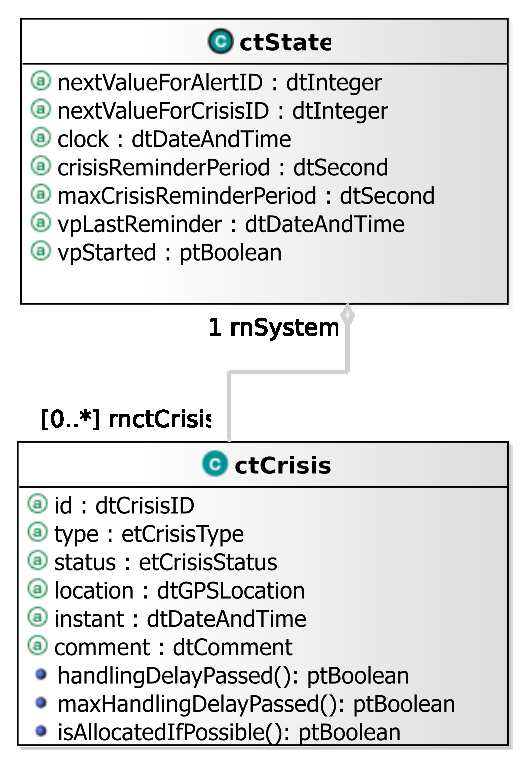
\includegraphics[
angle=0
,scale=0.75
]{./images-report-gen/operation-model/operation-scope-outactActivator-oeSollicitateCrisisHandling.eps}
\end{center}
\caption[lu.uni.lassy.excalibur.examples.icrash Operation Scope: operation-scope-outactActivator-oeSollicitateCrisisHandling]{oeSollicitateCrisisHandling operation scope
}
\label{fig:lu.uni.lassy.excalibur.examples.icrash-OM-scopeView-operation-scope-outactActivator-oeSollicitateCrisisHandling}
\end{figure}
\vspace{0.5cm}


\section{Environment - Out Interface Operation Scheme for actAdministrator}
\label{OM-EM-OutInterface-OS-actAdministrator}
\subsection{Operation Model for oeAddCoordinator}

\label{OM-oeAddCoordinator}


The \msrcode{oeAddCoordinator} operation has the following properties:

	\begin{operationmodel}
	\addheading{Operation}
	\adddoublerow{oeAddCoordinator}{sent to add a new coordinator in the system's post state and environment's post state.}

	\addrowheading{Parameters}
	\addnumbereddoublerow{}{AdtCoordinatorID: dtCoordinatorID}{used to initialize the id field} 
	\addnumbereddoublerow{}{AdtLogin: dtLogin}{used to initialize the login field} 
	\addnumbereddoublerow{}{AdtPassword: dtPassword}{used to initialize the password field} 

	\addrowheading{Return type}
	\addsinglerow{ptBoolean}

	\addrowheading{Pre-Condition (protocol)}
	\addnumberedsinglerow{PreP}{the system is started}
	\addnumberedsinglerow{PreP}{the actor logged previously and did not log out ! (i.e. the associated ctAdministrator instance is considered logged)}
		
	\addrowheading{Pre-Condition (functional)}
	\addnumberedsinglerow{PreF}{ it is supposed that there cannot exist a ctCoordinator instance with the same \msrcode{id} attribute as the one the administrator wants to delete.}

	\addrowheading{Post-Condition (functional)}
	\addnumberedsinglerow{PostF}{ the environment has a new instance of coordinator actor allowing for input/output message communication with the system.}
	\addnumberedsinglerow{PostF}{the system's state has a new instance of ctCoordinator initialized with the given values.}
	\addnumberedsinglerow{PostF}{the new actor instance and ctCoordinator instance are related.}
	\addnumberedsinglerow{PostF}{the new actor instance and ctCoordinator instance are related according to the authenticated association.}
	\addnumberedsinglerow{PostF}{the administrator actor is informed about the satisfaction of its request.}

	\addrowheading{Post-Condition (protocol)}
	\addnumberedsinglerow{PostP}{ none}
	\end{operationmodel}



	% ------------------------------------------
	% MCL Listing
	% ------------------------------------------
	\vspace{1cm}
	The listing~\ref{OM-actAdministrator-oeAddCoordinator-MCL-LST} provides the \msrmessir (MCL-oriented) specification of the operation.
	
	\scriptsize
	\vspace{0.5cm}
	\begin{lstlisting}[style=MessirStyle,firstnumber=auto,captionpos=b,caption={\msrmessir (MCL-oriented) specification of the operation \emph{oeAddCoordinator}.},label=OM-actAdministrator-oeAddCoordinator-MCL-LST]

	/* Pre Protocol:*/ 
	preP{let TheSystem: ctState in
	  let TheActor:actAdministrator in
	  
	  self.rnActor.rnSystem = TheSystem
	  and self.rnActor = TheActor
	  
	/* PreP01 */
	  and TheSystem.vpStarted = true
	/* PreP02 */
	  and TheActor.rnctAuthenticated.vpIsLogged = true}
	
	/* Pre Functional:*/
	preF{let TheSystem: ctState in
	  let TheActor:actAdministrator in
	  let ColctCoordinators:Bag(ctCoordinator) in
	  
	  self.rnActor.rnSystem = TheSystem
	  and self.rnActor = TheActor
	/* PreF01 */
	  and TheSystem.rnctCoordinator->select(id.eq(AdtCoordinatorID))
	      = ColctCoordinators
	  and ColctCoordinators->isEmpty() = true}
	
	/* Post Functional:*/ 
	postF{let TheSystem: ctState in
	  let TheactCoordinator:actCoordinator in
	  let ThectCoordinator:ctCoordinator in
	  self.rnActor.rnSystem = TheSystem
	  and self.rnActor = TheActor
	/* PostF01 */
	  TheactCoordinator.init()
	/* PostF02 */
	  and ThectCoordinator.init(AdtCoordinatorID,AdtLogin,AdtPassword)
	
	/* PostF03 */
	  and TheactCoordinator@post.rnctCoordinator = ThectCoordinator
	  
	/* PostF04 */  
	  and ThectCoordinator@post.rnactAuthenticated = TheactCoordinator
	   
	/* PostF05 */  
	  and TheActor.rnInterfaceIN^ieCoordinatorAdded()}
	
	/* Post Protocol:*/ 
	postP{ true}
	
	\end{lstlisting}
	\normalsize 
	
	
	
	
	% ------------------------------------------
	% PROLOG Listing
	% ------------------------------------------
	
	\vspace{1cm}
	The listing~\ref{OM-actAdministrator-oeAddCoordinator-PROLOG-LST} provides the \msrmessir (Prolog-oriented) implementation of the operation.
	
	\scriptsize
	\vspace{0.5cm}
	
	\lstinputlisting[style=MessirPrologStyle,firstnumber=auto,captionpos=b,caption={\msrmessir (Prolog-oriented) implementation of the operation \emph{oeAddCoordinator}.},label=OM-actAdministrator-oeAddCoordinator-PROLOG-LST]{../lu.uni.lassy.excalibur.examples.icrash.simulation/src/Operations/Environment/OUT/outactAdministrator-oeAddCoordinator.pl}
	\normalsize






\subsection{Operation Model for oeDeleteCoordinator}

\label{OM-oeDeleteCoordinator}


The \msrcode{oeDeleteCoordinator} operation has the following properties:

	\begin{operationmodel}
	\addheading{Operation}
	\adddoublerow{oeDeleteCoordinator}{sent to delete an existing coordinator in the system's post state and environment's post state.}

	\addrowheading{Parameters}
	\addnumbereddoublerow{}{AdtCoordinatorID: dtCoordinatorID}{used for ctCoordinator instance retrieval} 

	\addrowheading{Return type}
	\addsinglerow{ptBoolean}

	\addrowheading{Pre-Condition (protocol)}
	\addnumberedsinglerow{PreP}{the system is started}
	\addnumberedsinglerow{PreP}{the actor logged previously and did not log out ! (i.e. the associated ctAdministrator instance is considered logged)}
		
	\addrowheading{Pre-Condition (functional)}
	\addnumberedsinglerow{PreF}{ it is supposed that there exist one ctCoordinator instance with the same \msrcode{id} attribute than the one the administrator wants to create.}

	\addrowheading{Post-Condition (functional)}
	\addnumberedsinglerow{PostF}{ the ctCoordinator class instance having the required id do not belong anymore to the post state as well as is related actCoordinator actor instance.}
	\addnumberedsinglerow{PostF}{the administrator actor is informed about the satisfaction of its request.}

	\addrowheading{Post-Condition (protocol)}
	\addnumberedsinglerow{PostP}{ none }
	\end{operationmodel}



	% ------------------------------------------
	% MCL Listing
	% ------------------------------------------
	\vspace{1cm}
	The listing~\ref{OM-actAdministrator-oeDeleteCoordinator-MCL-LST} provides the \msrmessir (MCL-oriented) specification of the operation.
	
	\scriptsize
	\vspace{0.5cm}
	\begin{lstlisting}[style=MessirStyle,firstnumber=auto,captionpos=b,caption={\msrmessir (MCL-oriented) specification of the operation \emph{oeDeleteCoordinator}.},label=OM-actAdministrator-oeDeleteCoordinator-MCL-LST]

	/* Pre Protocol:*/ 
	preP{let TheSystem: ctState in
	  let TheActor:actAdministrator in
	  
	  self.rnActor.rnSystem = TheSystem
	  and self.rnActor = TheActor
	  
	/* PreP01 */
	  and TheSystem.vpStarted = true
	/* PreP02 */
	  and TheActor.rnctAuthenticated.vpIsLogged = true}
	
	/* Pre Functional:*/
	preF{let TheSystem: ctState in
	  let TheActor:actAdministrator in
	   
	  self.rnActor.rnSystem = TheSystem
	  and self.rnActor = TheActor
	/* PreF01 */
	  TheSystem.rnctCoordinator->select(id.eq(AdtCoordinatorID))
	  = ColctCoordinators
	  and ColctCoordinators->size().eq(1)}
	
	/* Post Functional:*/ 
	postF{let TheSystem: ctState in
	  let TheActor:actAdministrator in
	  let ThectCoordinator:ctCoordinator in
	  self.rnActor.rnSystem = TheSystem
	  and self.rnActor = TheActor
	/* PostF01 */
	  TheSystem.rnctCoordinator->select(id.eq(AdtCoordinatorID))
	  = ThectCoordinator
	  and ThectCoordinator.rnactCoordinator->forAll(msrIsKilled)
	  and ThectCoordinator.msrIsKilled
	 
	  /* PostF02 */
	  and TheActor.rnInterfaceIN^ieCoordinatorDeleted()
	
	 /* Post Protocol:*/
	/* PostP01 */
	 and true}
	
	/* Post Protocol:*/ 
	postP{ true}
	
	\end{lstlisting}
	\normalsize 
	
	
	
	
	% ------------------------------------------
	% PROLOG Listing
	% ------------------------------------------
	
	\vspace{1cm}
	The listing~\ref{OM-actAdministrator-oeDeleteCoordinator-PROLOG-LST} provides the \msrmessir (Prolog-oriented) implementation of the operation.
	
	\scriptsize
	\vspace{0.5cm}
	
	\lstinputlisting[style=MessirPrologStyle,firstnumber=auto,captionpos=b,caption={\msrmessir (Prolog-oriented) implementation of the operation \emph{oeDeleteCoordinator}.},label=OM-actAdministrator-oeDeleteCoordinator-PROLOG-LST]{../lu.uni.lassy.excalibur.examples.icrash.simulation/src/Operations/Environment/OUT/outactAdministrator-oeDeleteCoordinator.pl}
	\normalsize






\subsection{Operation Model for oeLoginRecov}

\label{OM-oeLoginRecov}


The \msrcode{oeLoginRecov} operation has the following properties:

	\begin{operationmodel}
	\addheading{Operation}
	\adddoublerow{oeLoginRecov}{Verification of Login and Keyword}

	\addrowheading{Parameters}
	\addnumbereddoublerow{}{AdtLogin: dtLogin}{} 
	\addnumbereddoublerow{}{AdtKeyWord: dtKeyWord}{} 

	\addrowheading{Return type}
	\addsinglerow{ptBoolean}

	\addrowheading{Pre-Condition (protocol)}
	\addnumberedsinglerow{PreP}{System is started}
		
	\addrowheading{Pre-Condition (functional)}
	\addnumberedsinglerow{PreF}{none}

	\addrowheading{Post-Condition (functional)}
	\addnumberedsinglerow{PostF}{Capability to update the administrator password and matching confirmation}

	\addrowheading{Post-Condition (protocol)}
	\addnumberedsinglerow{PostP}{Value of vpIsLogged field of a current actor actAdministrator is set to true if validation is successful.}
	\end{operationmodel}



	% ------------------------------------------
	% MCL Listing
	% ------------------------------------------
	\vspace{1cm}
	The listing~\ref{OM-actAdministrator-oeLoginRecov-MCL-LST} provides the \msrmessir (MCL-oriented) specification of the operation.
	
	\scriptsize
	\vspace{0.5cm}
	\begin{lstlisting}[style=MessirStyle,firstnumber=auto,captionpos=b,caption={\msrmessir (MCL-oriented) specification of the operation \emph{oeLoginRecov}.},label=OM-actAdministrator-oeLoginRecov-MCL-LST]

	/* Pre Protocol:*/ 
	preP{let TheSystem: ctState in
					let TheActor:actAdministrator in
					self.rnActor.rnSystem = TheSystem
	 				and self.rnActor = TheActor
	 				
	 				/* PreP01 */
	  				and TheSystem.vpStarted = true
					/* PreP02 */
	 				 and TheActor.rnctAuthenticated.vpIsLogged = false}
	
	
	/* Post Functional:*/ 
	postF{let TheSystem: ctState in
	  				let AptStringMessageForTheactAdministrator:ptString in
	  
	  				self.rnActor.rnSystem = TheSystem
	 				and self.rnActor = TheActor
	  
	  				and /* PostF01 */
	   				   if (TheactAuthenticated.rnctAuthenticated.keyWord
	         				 = AdtKeyword
	          				and TheactAuthenticated.rnctAuthenticated.login
	             			 = AdtLogin
	     				    )
	     			 then (AptStringMessageForTheactLoginRecov.eq('Write your new password here...')
	          			  and TheactLogingRecov.rnInterfaceIN^ieMessage(AptStringMessageForTheactLoginRecov)
	          			 )
	      			else (AptStringMessageForTheactLoginRecov
	          			  .eq('Wrong identification information ! Please try again ...')
	          			  and TheactLoginRecov.rnInterfaceIN^ieMessage(AptStringMessageForTheactLoginRecov)
	           			 and AptStringMessageForTheactAdministrator.eq('Intrusion tentative !')
	          			  and TheSystem.rnactAdministrator
	           			     .rnInterfaceIN^ieMessage(AptStringMessageForTheactAdministrator)
						
	           		and /* PostF02 */
	           		and oeLoginRecov = true
	           )
	      endif}
	
	
	\end{lstlisting}
	\normalsize 
	
	
	
	






\subsection{Operation Model for oeUpdatePass}

\label{OM-oeUpdatePass}


The \msrcode{oeUpdatePass} operation has the following properties:

	\begin{operationmodel}
	\addheading{Operation}
	\adddoublerow{oeUpdatePass}{Update the administrator password and matching confirmation}

	\addrowheading{Parameters}
	\addnumbereddoublerow{}{AdtPassword: dtPassword}{New password for administrator} 
	\addnumbereddoublerow{}{AdtKeyWord: dtKeyWord}{Keyword which an administrator already has} 

	\addrowheading{Return type}
	\addsinglerow{ptBoolean}

	\addrowheading{Pre-Condition (protocol)}
	\addnumberedsinglerow{PreP}{System is started}
	\addnumberedsinglerow{PreP}{The actor is not logged in}
	\addnumberedsinglerow{PreP}{Value of vpIsLogged field for current actor actAdministrator is true}
		
	\addrowheading{Pre-Condition (functional)}
	\addnumberedsinglerow{PreF}{none}

	\addrowheading{Post-Condition (functional)}
	\addnumberedsinglerow{PostF}{none}

	\addrowheading{Post-Condition (protocol)}
	\addnumberedsinglerow{PostP}{The administrator password has changed}
	\end{operationmodel}



	% ------------------------------------------
	% MCL Listing
	% ------------------------------------------
	\vspace{1cm}
	The listing~\ref{OM-actAdministrator-oeUpdatePass-MCL-LST} provides the \msrmessir (MCL-oriented) specification of the operation.
	
	\scriptsize
	\vspace{0.5cm}
	\begin{lstlisting}[style=MessirStyle,firstnumber=auto,captionpos=b,caption={\msrmessir (MCL-oriented) specification of the operation \emph{oeUpdatePass}.},label=OM-actAdministrator-oeUpdatePass-MCL-LST]

	/* Pre Protocol:*/ 
	preP{let TheSystem: ctState in
					let TheActor:actAdministrator in
					self.rnActor.rnSystem = TheSystem
	 				and self.rnActor = TheActor
	 				
	 				/* PreP01 */
	  				and TheSystem.vpStarted = true
					/* PreP02 */
	 				 and TheActor.rnctAuthenticated.vpIsLogged = false
	  				/* PreP03 */
	  				and oeLoginRecov = true}
	
	
	
	
	\end{lstlisting}
	\normalsize 
	
	
	
	






\section{Environment - Out Interface Operation Scheme for actAuthenticated}
\label{OM-EM-OutInterface-OS-actAuthenticated}
\subsection{Operation Model for oeLogin}

\label{OM-oeLogin}


The \msrcode{oeLogin} operation has the following properties:

	\begin{operationmodel}
	\addheading{Operation}
	\adddoublerow{oeLogin}{sent to request authorization to request access secured system operations.}

	\addrowheading{Parameters}
	\addnumbereddoublerow{}{AdtLogin: dtLogin}{first information used to determine accessibility rights for the actual actor.} 
	\addnumbereddoublerow{}{AdtPassword: dtPassword}{second information used to determine accessibility rights for the actual actor.} 

	\addrowheading{Return type}
	\addsinglerow{ptBoolean}

	\addrowheading{Pre-Condition (protocol)}
	\addnumberedsinglerow{PreP}{the system is started}
	\addnumberedsinglerow{PreP}{the actor is not already logged in ! (i.e. the associated ctAuthenticated instance is not considered logged)}
		
	\addrowheading{Pre-Condition (functional)}
	\addnumberedsinglerow{PreF}{none }

	\addrowheading{Post-Condition (functional)}
	\addnumberedsinglerow{PostF}{ if the login and password provided by the actor correspond to the ones that belong to the ctAuthenticated instance he is related to 
	then a welcome message is sent to the actor (n.b. the logged status is changed as a post-protocol condition);
	else the actor is notified that he gave incorrect data and all the administrator actors existing in the environement are notified of an intrusion temptative.}

	\addrowheading{Post-Condition (protocol)}
	\addnumberedsinglerow{PostP}{if the authentication information is correct then the actor is known to be logged in ! (i.e. the associated ctAuthenticated instance with given login and password is considered logged)}
	\end{operationmodel}



	% ------------------------------------------
	% MCL Listing
	% ------------------------------------------
	\vspace{1cm}
	The listing~\ref{OM-actAuthenticated-oeLogin-MCL-LST} provides the \msrmessir (MCL-oriented) specification of the operation.
	
	\scriptsize
	\vspace{0.5cm}
	\begin{lstlisting}[style=MessirStyle,firstnumber=auto,captionpos=b,caption={\msrmessir (MCL-oriented) specification of the operation \emph{oeLogin}.},label=OM-actAuthenticated-oeLogin-MCL-LST]

	/* Pre Protocol:*/ 
	preP{let TheSystem: ctState in
	  let TheActor:actAuthenticated in
	  self.rnActor.rnSystem = TheSystem
	  and self.rnActor = TheActor
	  
	/* PreP01 */
	  and TheSystem.vpStarted = true
	/* PreP02 */
	  and TheActor.rnctAuthenticated.vpIsLogged = false}
	
	/* Pre Functional:*/
	preF{/* PreF01 */
	true}
	
	/* Post Functional:*/ 
	postF{let TheSystem: ctState in
	  let TheactAuthenticated:actAuthenticated in
	
	  let AptStringMessageForTheactAuthenticated: ptString in
	  let AptStringMessageForTheactAdministrator:ptString in
	  
	  self.rnActor.rnSystem = TheSystem
	  and self.rnActor = TheactAuthenticated
	  
	  and /* PostF01 */
	      if (TheactAuthenticated.rnctAuthenticated.pwd
	          = AdtPassword
	          and TheactAuthenticated.rnctAuthenticated.login
	              = AdtLogin
	         )
	      then (AptStringMessageForTheactAuthenticated.eq('You are logged ! Welcome ...')
	            and TheactAuthenticated.rnInterfaceIN^ieMessage(AptStringMessageForTheactAuthenticated)
	           )
	      else (AptStringMessageForTheactAuthenticated
	            .eq('Wrong identification information ! Please try again ...')
	            and TheactAuthenticated.rnInterfaceIN^ieMessage(AptStringMessageForTheactAuthenticated)
	            and AptStringMessageForTheactAdministrator.eq('Intrusion tentative !')
	            and TheSystem.rnactAdministrator
	                .rnInterfaceIN^ieMessage(AptStringMessageForTheactAdministrator)
	           )
	      endif}
	
	/* Post Protocol:*/ 
	postP{ let TheSystem: ctState in
	  let TheactAuthenticated:actAuthenticated in
	
	  self.rnActor.rnSystem = TheSystem
	  and self.rnActor = TheactAuthenticated
	/* PostP01 */
	  if (TheactAuthenticated.rnctAuthenticated.pwd = AdtPassword
	      and TheactAuthenticated.rnctAuthenticated.login = AdtLogin
	     )
	  then (TheactAuthenticated.rnctAuthenticated@post.vpIsLogged = true)
	  else true
	  endif}
	
	\end{lstlisting}
	\normalsize 
	
	
	
	
	% ------------------------------------------
	% PROLOG Listing
	% ------------------------------------------
	
	\vspace{1cm}
	The listing~\ref{OM-actAuthenticated-oeLogin-PROLOG-LST} provides the \msrmessir (Prolog-oriented) implementation of the operation.
	
	\scriptsize
	\vspace{0.5cm}
	
	\lstinputlisting[style=MessirPrologStyle,firstnumber=auto,captionpos=b,caption={\msrmessir (Prolog-oriented) implementation of the operation \emph{oeLogin}.},label=OM-actAuthenticated-oeLogin-PROLOG-LST]{../lu.uni.lassy.excalibur.examples.icrash.simulation/src/Operations/Environment/OUT/outactAuthenticated-oeLogin.pl}
	\normalsize






\subsection{Operation Model for oeLogout}

\label{OM-oeLogout}


The \msrcode{oeLogout} operation has the following properties:

	\begin{operationmodel}
	\addheading{Operation}
	\adddoublerow{oeLogout}{sent to end the secured access to specific system operations.}


	\addrowheading{Return type}
	\addsinglerow{ptBoolean}

	\addrowheading{Pre-Condition (protocol)}
	\addnumberedsinglerow{PreP}{the system is started}
	\addnumberedsinglerow{PreP}{the actor is currently logged in ! (i.e. the associated ctAuthenticated instance is considered logged)}
		
	\addrowheading{Pre-Condition (functional)}
	\addnumberedsinglerow{PreF}{ }

	\addrowheading{Post-Condition (functional)}
	\addnumberedsinglerow{PostF}{a logout confirmation message is sent to the actor (n.b. the logged status is changed as a post-protocol condition)}

	\addrowheading{Post-Condition (protocol)}
	\addnumberedsinglerow{PostP}{the actor is known to be logged out ! (i.e. the associated ctAuthenticated instance with given login and password is considered logged out)}
	\end{operationmodel}



	% ------------------------------------------
	% MCL Listing
	% ------------------------------------------
	\vspace{1cm}
	The listing~\ref{OM-actAuthenticated-oeLogout-MCL-LST} provides the \msrmessir (MCL-oriented) specification of the operation.
	
	\scriptsize
	\vspace{0.5cm}
	\begin{lstlisting}[style=MessirStyle,firstnumber=auto,captionpos=b,caption={\msrmessir (MCL-oriented) specification of the operation \emph{oeLogout}.},label=OM-actAuthenticated-oeLogout-MCL-LST]

	/* Pre Protocol:*/ 
	preP{let TheSystem: ctState in
	  let TheActor:actAdministrator in
	  self.rnActor.rnSystem = TheSystem
	  and self.rnActor = TheActor
	  
	/* PreP01 */
	  and TheSystem.vpStarted = true
	/* PreP02 */
	  and TheActor.rnctAuthenticated.vpIsLogged = true}
	
	/* Pre Functional:*/
	preF{/* PreF01 */
	true}
	
	/* Post Functional:*/ 
	postF{let TheSystem: ctState in
	  let TheactAuthenticated:actAuthenticated in
	  let AptStringMessageForTheactAuthenticated: ptString in
	  
	  self.rnActor.rnSystem = TheSystem
	  and self.rnActor = TheactAuthenticated
	  
	  /* PostF01 */
	  AptStringMessageForTheactAuthenticated.eq('You are logged out ! Good Bye ...')
	  and TheactAuthenticated.rnInterfaceIN^ieMessage(AptStringMessageForTheactAuthenticated)}
	
	/* Post Protocol:*/ 
	postP{ let TheSystem: ctState in
	  let TheactAuthenticated:actAuthenticated in
	
	  self.rnActor.rnSystem = TheSystem
	  and self.rnActor = TheactAuthenticated.asSet
	/* PostP01 */
	  TheactAuthenticated.rnctAuthenticated@post.vpIsLogged = false}
	
	\end{lstlisting}
	\normalsize 
	
	
	
	
	% ------------------------------------------
	% PROLOG Listing
	% ------------------------------------------
	
	\vspace{1cm}
	The listing~\ref{OM-actAuthenticated-oeLogout-PROLOG-LST} provides the \msrmessir (Prolog-oriented) implementation of the operation.
	
	\scriptsize
	\vspace{0.5cm}
	
	\lstinputlisting[style=MessirPrologStyle,firstnumber=auto,captionpos=b,caption={\msrmessir (Prolog-oriented) implementation of the operation \emph{oeLogout}.},label=OM-actAuthenticated-oeLogout-PROLOG-LST]{../lu.uni.lassy.excalibur.examples.icrash.simulation/src/Operations/Environment/OUT/outactAuthenticated-oeLogout.pl}
	\normalsize






\section{Environment - Out Interface Operation Scheme for actComCompany}
\label{OM-EM-OutInterface-OS-actComCompany}
\subsection{Operation Model for oeAlert}

\label{OM-oeAlert}


The \msrcode{oeAlert} operation has the following properties:

	\begin{operationmodel}
	\addheading{Operation}
	\adddoublerow{oeAlert}{Any human having a phone able to connect to the communication companies using the \msricrash system can send his company an sms message with structured information in order to declare an alert.}

	\addrowheading{Parameters}
	\addnumbereddoublerow{}{AetHumanKind: etHumanKind}{the kind of human informing of an alert.} 
	\addnumbereddoublerow{}{AdtDate: dtDate}{the date of the alert } 
	\addnumbereddoublerow{}{AdtTime: dtTime}{the time of the alert} 
	\addnumbereddoublerow{}{AdtPhoneNumber: dtPhoneNumber}{the phone number of the human sending the alert SMS message } 
	\addnumbereddoublerow{}{AdtGPSLocation: dtGPSLocation}{ the GPS position of the phone at the date and time the message was sent.} 
	\addnumbereddoublerow{}{AdtComment: dtComment}{a free text message sent by the human providing information on the alert that he wants to declare} 

	\addrowheading{Return type}
	\addsinglerow{ptBoolean}

	\addrowheading{Pre-Condition (protocol)}
	\addnumberedsinglerow{PreP}{ the system is supposed to be created and initialized.}
		
	\addrowheading{Pre-Condition (functional)}
	\addnumberedsinglerow{PreF}{ the date and time the alert is declared is supposed to be in the past with respect to the current time known by the system.}

	\addrowheading{Post-Condition (functional)}
	\addnumberedsinglerow{PostF}{ the ctState attribute for the next value for alert IDs is incremented by one at post.}
	\addnumberedsinglerow{PostF}{ a new alert instance exists in the post state with status pending, instant information (resp. GPS location and comment) based on date and time provided (resp. position and comment); and with alert ID being a string conversion of the dtInteger value available in the pre state in the ctState instance.}
	\addnumberedsinglerow{PostF}{if there exist no already registered alert near to the alert currently declared
	then a new crisis is added in the post state and initialized with: its ID being the one provided by the ctState instance (which is incremented by one in the post state), its type considered as small, its status being pending, its declared time being the same than the alert and a default comment indicating that a report will come later on.
	else the crisis to which the new alert must be related to is the one related to any alert nearby in the pre-state.}
	\addnumberedsinglerow{PostF}{the post state relates the new alert to the previously characterized crisis.}
	\addnumberedsinglerow{PostF}{if there is no ctHuman instance having same phone number and same kind in the pre-state 
	then a new one is added in the post-state with given phone number and kind and is associated to the communication company actor used to declare the alert.
	else the pre-state one is chosen
	}
	\addnumberedsinglerow{PostF}{and this specified ctHuman is related to the new alert thus indicating he has signled the alert. }

	\addrowheading{Post-Condition (protocol)}
	\addnumberedsinglerow{PostP}{ none}
	\end{operationmodel}



	% ------------------------------------------
	% MCL Listing
	% ------------------------------------------
	\vspace{1cm}
	The listing~\ref{OM-actComCompany-oeAlert-MCL-LST} provides the \msrmessir (MCL-oriented) specification of the operation.
	
	\scriptsize
	\vspace{0.5cm}
	\begin{lstlisting}[style=MessirStyle,firstnumber=auto,captionpos=b,caption={\msrmessir (MCL-oriented) specification of the operation \emph{oeAlert}.},label=OM-actComCompany-oeAlert-MCL-LST]

	/* Pre Protocol:*/ 
	preP{let TheSystem: ctState in
	  self.rnActor.rnSystem = TheSystem
	  
	/* PreP01 */
	  and TheSystem.vpStarted = true}
	
	/* Pre Functional:*/
	preF{let TheSystem: ctState in
	  self.rnActor.rnSystem = TheSystem
	
	/* PreF01 */
	  and (TheSystem.clock.date.gt(AdtDate)
	       or (TheSystem.clock.date.eq(AdtDate)
	           and TheSystem.clock.time.gt(AdtTime)
	          )
	      )}
	
	/* Post Functional:*/ 
	postF{let TheSystem: ctState in
	  
	 let  ActHuman:ctHuman in
	 let  TheactComCompany:actComCompany in
	 let  ActAlert:ctAlert in
	 let  AAlertInstant:dtDateAndTime in
	 let  AetAlertStatus:etAlertStatus in
	 let  ActAlertNearBy:ctAlert in
	 let  ActCrisis:ctCrisis in
	 let  AdtCrisisID:dtCrisisID in
	 let  AetCrisisType:etCrisisType in
	 let  AetCrisisStatus:etCrisisStatus in
	 let  ACrisisInstant:dtDateAndTime in
	 let  ACrisisdtComment:dtComment in
	 let  AptStringMessage:ptString in
	 let  AdtSMS:dtSMS in
	 let  AdtAlertID:dtAlertID in
	 
	  self.rnActor.rnSystem = TheSystem
	  and self.rnActor = TheactComCompany
	/* PostF01 */
	 TheSystem.nextValueForAlertID=PrenextValueForAlertID
	 and PrenextValueForAlertID.add(1) = PostnextValueForAlertID
	 and TheSystem@post.nextValueForAlertID = PostnextValueForAlertID
	
	
	  /* PostF02 */
	and AAlertInstant.date=AdtDate
	and AAlertInstant.time=AdtTime
	
	and AetAlertStatus=pending
	        
	and TheSystem.nextValueForAlertID.todtString().eq(AdtAlertID)
	
	and ActAlert.init(AdtAlertID,
	                  AetAlertStatus,
	                  AdtGPSLocation,
	                  AAlertInstant,
	                  AdtComment)
	      
	  /* PostF03 */
	and TheSystem.rnctAlert.select(location.isNearTo(AdtGPSLocation)) = ColctAlertsNearBy
	and if  (ColctAlertsNearBy->size()=0)
	    then (TheSystem.nextValueForCrisisID = PrenextValueForCrisisID
	          and PrenextValueForCrisisID.add(1) = PostnextValueForCrisisID
	          and TheSystem@post.nextValueForCrisisID = PostnextValueForCrisisID
	          and TheSystem.nextValueForCrisisID.todtString().eq(AdtCrisisID)
	          and AdtCrisisType = small
	          and AetCrisisStatus = pending
	          and ACrisisInstant= AAlertInstant
	          and ACrisisdtComment = 'no reporting yet defined'
	          and ActCrisis.init( AdtCrisisID,
	                              AdtCrisisType,
	                              AetCrisisStatus,
	                              AdtGPSLocation,
	                              ACrisisInstant,
	                              ACrisisdtComment)
	         )
	  else (ColctAlertsNearBy.rnTheCrisis->msrAny(true) = ActCrisis)
	  endif
	
	  /* PostF04 */
	and ActAlert@post.rnTheCrisis = ActCrisis
	      
	/* PostF05 */
	and  TheSystem.rnctHuman->select(id.eq(AdtPhoneNumber)) = HumanCol1
	
	and HumanCol1->select(kind.etEq(AetHumanKind)) = HumanCol2
	and if (HumanCol2->msrIsEmpty)
	    then (ActHuman.init(AdtPhoneNumber,AetHumanKind)
	          and ActHuman@post.rnactComCompany = TheactComCompany
	         )
	    else (HumanCol2->any(true) = ActHuman)
	    endif
	    
	 and ActHuman.rnSignaled->msrIncluding(ActAlert) = ColAlerts
	 
	 and ActHuman@post.rnSignaled = ColAlerts
	
	/* PostF06 */
	AdtSMS.value = 'Your alert has been registered. We will handle it and keep you informed'
	and TheactComCompany.rnInterfaceIN^ieSmsSend(AdtPhoneNumber,AdtSMS)}
	
	/* Post Protocol:*/ 
	postP{ true}
	
	\end{lstlisting}
	\normalsize 
	
	
	
	
	% ------------------------------------------
	% PROLOG Listing
	% ------------------------------------------
	
	\vspace{1cm}
	The listing~\ref{OM-actComCompany-oeAlert-PROLOG-LST} provides the \msrmessir (Prolog-oriented) implementation of the operation.
	
	\scriptsize
	\vspace{0.5cm}
	
	\lstinputlisting[style=MessirPrologStyle,firstnumber=auto,captionpos=b,caption={\msrmessir (Prolog-oriented) implementation of the operation \emph{oeAlert}.},label=OM-actComCompany-oeAlert-PROLOG-LST]{../lu.uni.lassy.excalibur.examples.icrash.simulation/src/Operations/Environment/OUT/outactComCompany-oeAlert.pl}
	\normalsize





Figure \ref{fig:lu.uni.lassy.excalibur.examples.icrash-OM-scopeView-operation-scope-outactComCompany-oeAlertv2}
shows concept model elements in the scope of the oeAlert operation

\begin{figure}[htbp]
\begin{center}

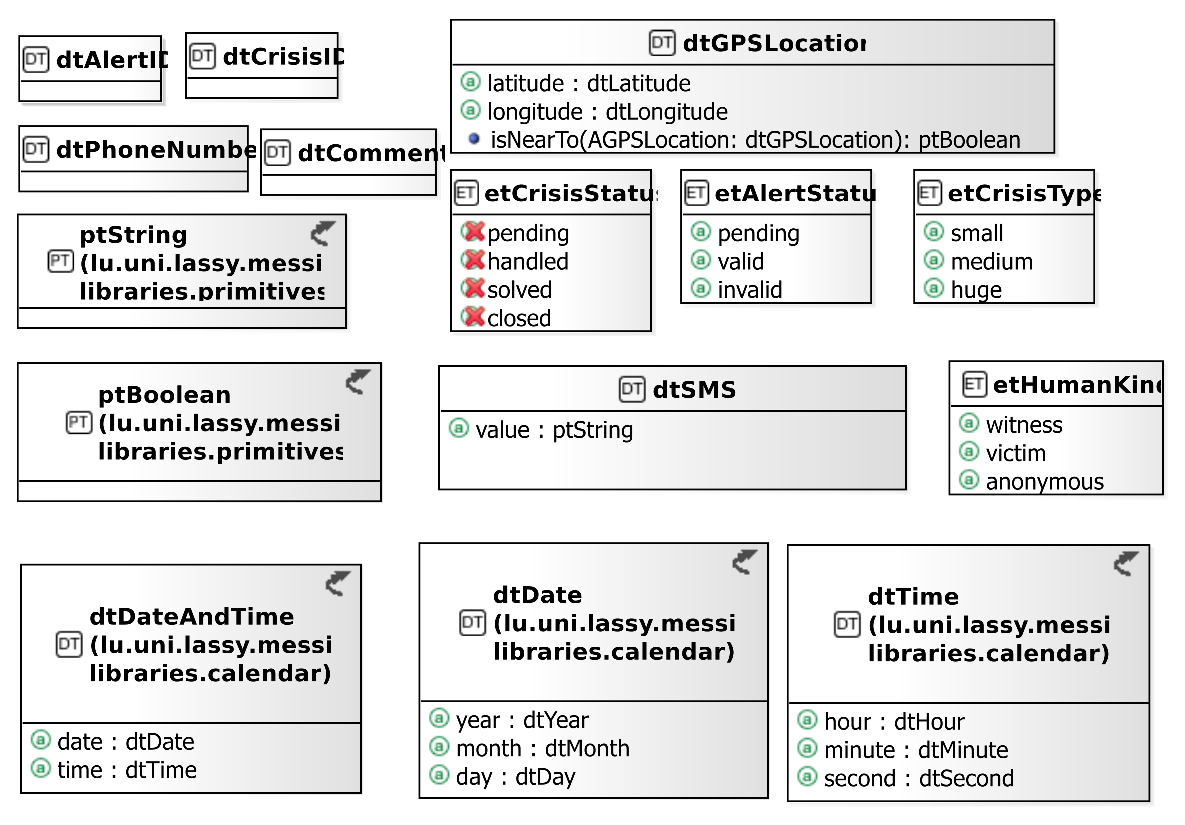
\includegraphics[
angle=0
,width=1.0\textwidth
]{./images-report-gen/operation-model/operation-scope-outactComCompany-oeAlertv2.eps}
\end{center}
\caption[lu.uni.lassy.excalibur.examples.icrash Operation Scope: operation-scope-outactComCompany-oeAlertv2]{oeAlert operation scope
}
\label{fig:lu.uni.lassy.excalibur.examples.icrash-OM-scopeView-operation-scope-outactComCompany-oeAlertv2}
\end{figure}
\vspace{0.5cm}

Figure \ref{fig:lu.uni.lassy.excalibur.examples.icrash-OM-scopeView-operation-scope-outactComCompany-oeAlertv3}
shows concept model elements in the scope of the oeAlert operation

\begin{figure}[htbp]
\begin{center}

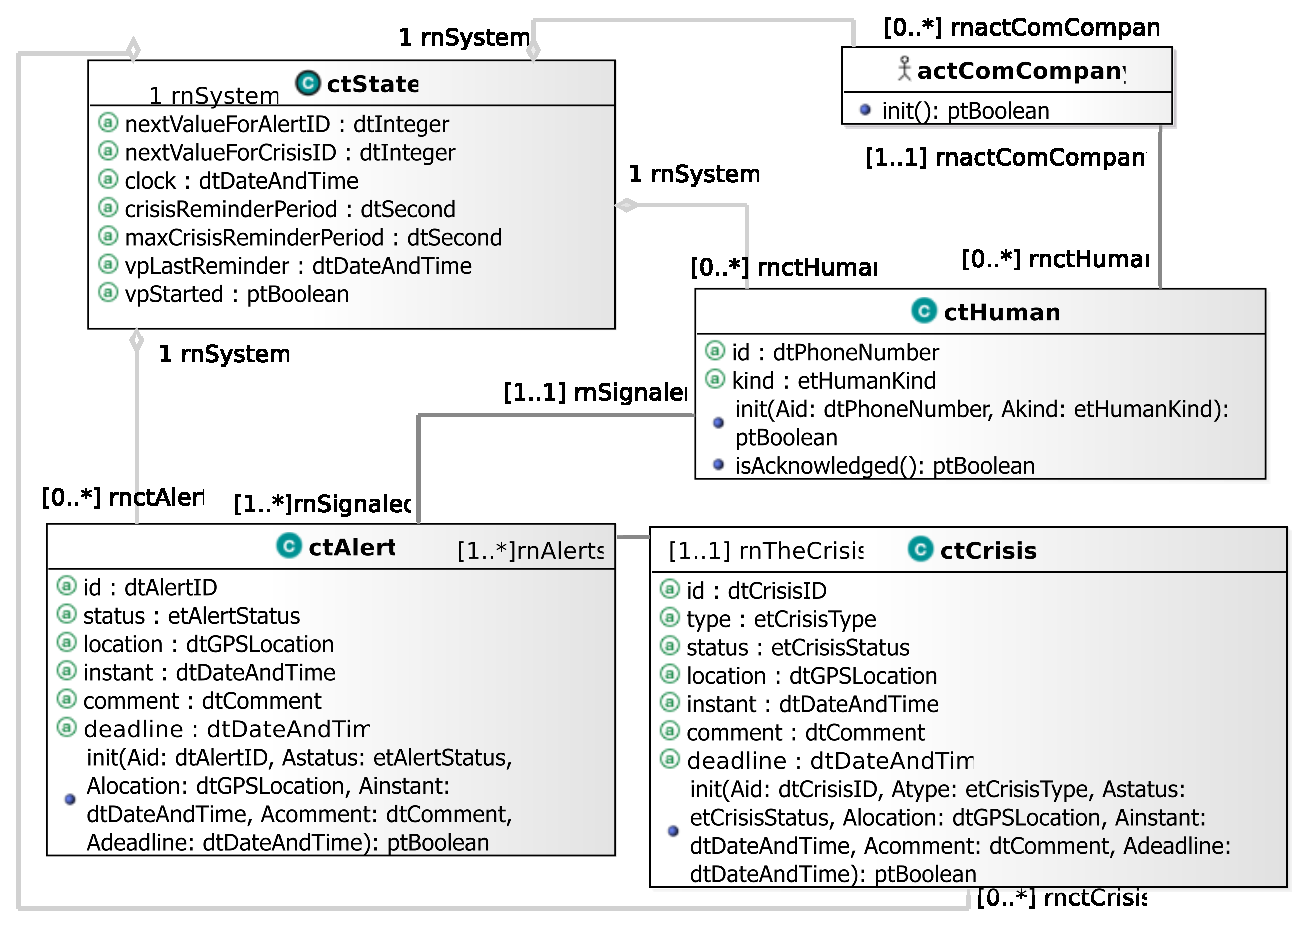
\includegraphics[
angle=0
,width=1.0\textwidth
]{./images-report-gen/operation-model/operation-scope-outactComCompany-oeAlertv3.eps}
\end{center}
\caption[lu.uni.lassy.excalibur.examples.icrash Operation Scope: operation-scope-outactComCompany-oeAlertv3]{oeAlert operation scope
}
\label{fig:lu.uni.lassy.excalibur.examples.icrash-OM-scopeView-operation-scope-outactComCompany-oeAlertv3}
\end{figure}
\vspace{0.5cm}


\section{Environment - Out Interface Operation Scheme for actCoordinator}
\label{OM-EM-OutInterface-OS-actCoordinator}
\subsection{Operation Model for oeCloseCrisis}

\label{OM-oeCloseCrisis}


The \msrcode{oeCloseCrisis} operation has the following properties:

	\begin{operationmodel}
	\addheading{Operation}
	\adddoublerow{oeCloseCrisis}{sent to indicate that a crisis should be considered as closed.}

	\addrowheading{Parameters}
	\addnumbereddoublerow{}{AdtCrisisID: dtCrisisID}{the identification information used to determine the crisis to close} 

	\addrowheading{Return type}
	\addsinglerow{ptBoolean}

	\addrowheading{Pre-Condition (protocol)}
	\addnumberedsinglerow{PreP}{the system is started}
	\addnumberedsinglerow{PreP}{the actor logged previously and did not log out ! (i.e. the associated ctCoordinator instance is considered logged)}
		
	\addrowheading{Pre-Condition (functional)}
	\addnumberedsinglerow{PreF}{it is supposed that there exist one ctCrisis instance with the same \msrcode{id} attribute value as the one provided by the coordinator actor who wants to close.}

	\addrowheading{Post-Condition (functional)}
	\addnumberedsinglerow{PostF}{the ctCrisis class instance having the provided id is considered closed in the post state.}
	\addnumberedsinglerow{PostF}{There is no handler declared in the system as associated to the crisis.}
	\addnumberedsinglerow{PostF}{all the alert instances associated to this crisis do not belong any more to the system's post state.}
	\addnumberedsinglerow{PostF}{the coordinator actor is informed about the satisfaction of its request.}

	\addrowheading{Post-Condition (protocol)}
	\addnumberedsinglerow{PostP}{none}
	\end{operationmodel}



	
	
	
	
	% ------------------------------------------
	% PROLOG Listing
	% ------------------------------------------
	
	\vspace{1cm}
	The listing~\ref{OM-actCoordinator-oeCloseCrisis-PROLOG-LST} provides the \msrmessir (Prolog-oriented) implementation of the operation.
	
	\scriptsize
	\vspace{0.5cm}
	
	\lstinputlisting[style=MessirPrologStyle,firstnumber=auto,captionpos=b,caption={\msrmessir (Prolog-oriented) implementation of the operation \emph{oeCloseCrisis}.},label=OM-actCoordinator-oeCloseCrisis-PROLOG-LST]{../lu.uni.lassy.excalibur.examples.icrash.simulation/src/Operations/Environment/OUT/outactCoordinator-oeCloseCrisis.pl}
	\normalsize






\subsection{Operation Model for oeGetAlertsSet}

\label{OM-oeGetAlertsSet}


The \msrcode{oeGetAlertsSet} operation has the following properties:

	\begin{operationmodel}
	\addheading{Operation}
	\adddoublerow{oeGetAlertsSet}{sent to request all the ctAlert instances having a specific status.}

	\addrowheading{Parameters}
	\addnumbereddoublerow{}{AetAlertStatus: etAlertStatus}{the criteria used to select the alerts to send back to the actor} 

	\addrowheading{Return type}
	\addsinglerow{ptBoolean}

	\addrowheading{Pre-Condition (protocol)}
	\addnumberedsinglerow{PreP}{the system is started}
	\addnumberedsinglerow{PreP}{the actor logged previously and did not log out ! (i.e. the associated ctCoordinator instance is considered logged)}
		
	\addrowheading{Pre-Condition (functional)}
	\addnumberedsinglerow{PreF}{none}

	\addrowheading{Post-Condition (functional)}
	\addnumberedsinglerow{PostF}{ the post state is the one obtained by satisfying the \msrcode{isSentToCoordinator} predicate for each alert having the provided status and for the actor sending the message. (cf. specification of \msrcode{isSentToCoordinator} predicate given for the \msrcode{ctAlert} type.}

	\addrowheading{Post-Condition (protocol)}
	\addnumberedsinglerow{PostP}{ none}
	\end{operationmodel}



	
	
	
	
	% ------------------------------------------
	% PROLOG Listing
	% ------------------------------------------
	
	\vspace{1cm}
	The listing~\ref{OM-actCoordinator-oeGetAlertsSet-PROLOG-LST} provides the \msrmessir (Prolog-oriented) implementation of the operation.
	
	\scriptsize
	\vspace{0.5cm}
	
	\lstinputlisting[style=MessirPrologStyle,firstnumber=auto,captionpos=b,caption={\msrmessir (Prolog-oriented) implementation of the operation \emph{oeGetAlertsSet}.},label=OM-actCoordinator-oeGetAlertsSet-PROLOG-LST]{../lu.uni.lassy.excalibur.examples.icrash.simulation/src/Operations/Environment/OUT/outactCoordinator-oeGetAlertsSet.pl}
	\normalsize






\subsection{Operation Model for oeGetCrisisSet}

\label{OM-oeGetCrisisSet}


The \msrcode{oeGetCrisisSet} operation has the following properties:

	\begin{operationmodel}
	\addheading{Operation}
	\adddoublerow{oeGetCrisisSet}{sent to request all the ctCrisis instances having a specific status.}

	\addrowheading{Parameters}
	\addnumbereddoublerow{}{AetCrisisStatus: etCrisisStatus}{the status information used to determine the crisis to send back to the actor} 

	\addrowheading{Return type}
	\addsinglerow{ptBoolean}

	\addrowheading{Pre-Condition (protocol)}
	\addnumberedsinglerow{PreP}{the system is started}
	\addnumberedsinglerow{PreP}{the actor logged previously and did not log out ! (i.e. the associated ctCoordinator instance is considered logged)}
		
	\addrowheading{Pre-Condition (functional)}
	\addnumberedsinglerow{PreF}{none}

	\addrowheading{Post-Condition (functional)}
	\addnumberedsinglerow{PostF}{ the post state is the one obtained by satisfying the \msrcode{isSentToCoordinator} predicate for each crisis having the provided status and for the actor sending the message \msrcode{ieSendACrisis}. (cf. specification of \msrcode{isSentToCoordinator} predicate given for the \msrcode{ctCrisis} type.}

	\addrowheading{Post-Condition (protocol)}
	\addnumberedsinglerow{PostP}{ none}
	\end{operationmodel}



	
	
	
	
	% ------------------------------------------
	% PROLOG Listing
	% ------------------------------------------
	
	\vspace{1cm}
	The listing~\ref{OM-actCoordinator-oeGetCrisisSet-PROLOG-LST} provides the \msrmessir (Prolog-oriented) implementation of the operation.
	
	\scriptsize
	\vspace{0.5cm}
	
	\lstinputlisting[style=MessirPrologStyle,firstnumber=auto,captionpos=b,caption={\msrmessir (Prolog-oriented) implementation of the operation \emph{oeGetCrisisSet}.},label=OM-actCoordinator-oeGetCrisisSet-PROLOG-LST]{../lu.uni.lassy.excalibur.examples.icrash.simulation/src/Operations/Environment/OUT/outactCoordinator-oeGetCrisisSet.pl}
	\normalsize






\subsection{Operation Model for oeInvalidateAlert}

\label{OM-oeInvalidateAlert}


The \msrcode{oeInvalidateAlert} operation has the following properties:

	\begin{operationmodel}
	\addheading{Operation}
	\adddoublerow{oeInvalidateAlert}{ sent to indicate that an alert should be considered as closed.}

	\addrowheading{Parameters}
	\addnumbereddoublerow{}{AdtAlertID: dtAlertID}{the identification information used to determine the alert to close} 

	\addrowheading{Return type}
	\addsinglerow{ptBoolean}

	\addrowheading{Pre-Condition (protocol)}
	\addnumberedsinglerow{PreP}{the system is started}
	\addnumberedsinglerow{PreP}{the actor logged previously and did not log out ! (i.e. the associated ctCoordinator instance is considered logged)}
		
	\addrowheading{Pre-Condition (functional)}
	\addnumberedsinglerow{PreF}{ it is supposed that there exist one ctAlert instance with the same \msrcode{id} attribute value as the one provided by the coordinator actor who wants to close.}

	\addrowheading{Post-Condition (functional)}
	\addnumberedsinglerow{PostF}{the ctAlert class instance having the provided id is considered closed in the post state.}
	\addnumberedsinglerow{PostF}{the coordinator actor is informed about the satisfaction of its request.}

	\addrowheading{Post-Condition (protocol)}
	\addnumberedsinglerow{PostP}{ none}
	\end{operationmodel}



	
	
	
	
	% ------------------------------------------
	% PROLOG Listing
	% ------------------------------------------
	
	\vspace{1cm}
	The listing~\ref{OM-actCoordinator-oeInvalidateAlert-PROLOG-LST} provides the \msrmessir (Prolog-oriented) implementation of the operation.
	
	\scriptsize
	\vspace{0.5cm}
	
	\lstinputlisting[style=MessirPrologStyle,firstnumber=auto,captionpos=b,caption={\msrmessir (Prolog-oriented) implementation of the operation \emph{oeInvalidateAlert}.},label=OM-actCoordinator-oeInvalidateAlert-PROLOG-LST]{../lu.uni.lassy.excalibur.examples.icrash.simulation/src/Operations/Environment/OUT/outactCoordinator-oeInvalidateAlert.pl}
	\normalsize






\subsection{Operation Model for oeReportOnCrisis}

\label{OM-oeReportOnCrisis}


The \msrcode{oeReportOnCrisis} operation has the following properties:

	\begin{operationmodel}
	\addheading{Operation}
	\adddoublerow{oeReportOnCrisis}{sent to update the textual information available for a specific handled crisis.}

	\addrowheading{Parameters}
	\addnumbereddoublerow{}{AdtCrisisID: dtCrisisID}{the identification information used to determine the crisis to report on} 
	\addnumbereddoublerow{}{AdtComment: dtComment}{the textual information commenting the crisis} 

	\addrowheading{Return type}
	\addsinglerow{ptBoolean}

	\addrowheading{Pre-Condition (protocol)}
	\addnumberedsinglerow{PreP}{the system is started}
	\addnumberedsinglerow{PreP}{the actor logged previously and did not log out ! (i.e. the associated ctCoordinator instance is considered logged)}
		
	\addrowheading{Pre-Condition (functional)}
	\addnumberedsinglerow{PreF}{it is supposed that there exist one crisis in the pre state having the given id.}

	\addrowheading{Post-Condition (functional)}
	\addnumberedsinglerow{PostF}{the comment attribute of the crisis instance having the given id is replaced by the given one and the requesting actor is notified of this update.}

	\addrowheading{Post-Condition (protocol)}
	\addnumberedsinglerow{PostP}{ none}
	\end{operationmodel}



	
	
	
	
	% ------------------------------------------
	% PROLOG Listing
	% ------------------------------------------
	
	\vspace{1cm}
	The listing~\ref{OM-actCoordinator-oeReportOnCrisis-PROLOG-LST} provides the \msrmessir (Prolog-oriented) implementation of the operation.
	
	\scriptsize
	\vspace{0.5cm}
	
	\lstinputlisting[style=MessirPrologStyle,firstnumber=auto,captionpos=b,caption={\msrmessir (Prolog-oriented) implementation of the operation \emph{oeReportOnCrisis}.},label=OM-actCoordinator-oeReportOnCrisis-PROLOG-LST]{../lu.uni.lassy.excalibur.examples.icrash.simulation/src/Operations/Environment/OUT/outactCoordinator-oeReportOnCrisis.pl}
	\normalsize






\subsection{Operation Model for oeSetCrisisHandler}

\label{OM-oeSetCrisisHandler}


The \msrcode{oeSetCrisisHandler} operation has the following properties:

	\begin{operationmodel}
	\addheading{Operation}
	\adddoublerow{oeSetCrisisHandler}{sent to declare himself as been the handler of a crisis having the specified id.}

	\addrowheading{Parameters}
	\addnumbereddoublerow{}{AdtCrisisID: dtCrisisID}{the identification information used to determine the crisis} 

	\addrowheading{Return type}
	\addsinglerow{ptBoolean}

	\addrowheading{Pre-Condition (protocol)}
	\addnumberedsinglerow{PreP}{the system is started}
	\addnumberedsinglerow{PreP}{the actor logged previously and did not log out ! (i.e. the associated ctCoordinator instance is considered logged)}
		
	\addrowheading{Pre-Condition (functional)}
	\addnumberedsinglerow{PreF}{ there exist one crisis having the given id in the pre-state.}

	\addrowheading{Post-Condition (functional)}
	\addnumberedsinglerow{PostF}{the ctCrisis instance having the provided id is in handled status at poststate and is associated to the actor that sends the message (which himself is notified with a textual message as confirmation).}
	\addnumberedsinglerow{PostF}{All the alerts related to this crisis are sent to the actor such that he can decide how to handle them.}
	\addnumberedsinglerow{PostF}{if the crisis was already handled at pre-sate then the associated handler actor is notified about the change of handler for one of his crisis (n.b. it might be the same even if not relevant).}
	\addnumberedsinglerow{PostF}{a message is sent to the communication company for any human related to an alert associated to the crisis. A human will receive as many messages as alerts he sent despite the fact that they might relate to the same crisis (i.e. one alert, one acknoledgement).}

	\addrowheading{Post-Condition (protocol)}
	\addnumberedsinglerow{PostP}{ none}
	\end{operationmodel}



	
	
	
	
	% ------------------------------------------
	% PROLOG Listing
	% ------------------------------------------
	
	\vspace{1cm}
	The listing~\ref{OM-actCoordinator-oeSetCrisisHandler-PROLOG-LST} provides the \msrmessir (Prolog-oriented) implementation of the operation.
	
	\scriptsize
	\vspace{0.5cm}
	
	\lstinputlisting[style=MessirPrologStyle,firstnumber=auto,captionpos=b,caption={\msrmessir (Prolog-oriented) implementation of the operation \emph{oeSetCrisisHandler}.},label=OM-actCoordinator-oeSetCrisisHandler-PROLOG-LST]{../lu.uni.lassy.excalibur.examples.icrash.simulation/src/Operations/Environment/OUT/outactCoordinator-oeSetCrisisHandler.pl}
	\normalsize






\subsection{Operation Model for oeSetCrisisStatus}

\label{OM-oeSetCrisisStatus}


The \msrcode{oeSetCrisisStatus} operation has the following properties:

	\begin{operationmodel}
	\addheading{Operation}
	\adddoublerow{oeSetCrisisStatus}{sent to define the handling status of a specific crisis.}

	\addrowheading{Parameters}
	\addnumbereddoublerow{}{AdtCrisisID: dtCrisisID}{the identification information used to determine the crisis} 
	\addnumbereddoublerow{}{AetCrisisStatus: etCrisisStatus}{the new status value} 

	\addrowheading{Return type}
	\addsinglerow{ptBoolean}

	\addrowheading{Pre-Condition (protocol)}
	\addnumberedsinglerow{PreP}{the system is started}
	\addnumberedsinglerow{PreP}{the actor logged previously and did not log out ! (i.e. the associated ctCoordinator instance is considered logged)}
		
	\addrowheading{Pre-Condition (functional)}
	\addnumberedsinglerow{PreF}{it is supposed that there exist one crisis in the pre state having the given id.}

	\addrowheading{Post-Condition (functional)}
	\addnumberedsinglerow{PostF}{the crisis status attribute of the crisis instance having the given id is replaced by the given one and the requesting actor is notified of this update.}

	\addrowheading{Post-Condition (protocol)}
	\addnumberedsinglerow{PostP}{none}
	\end{operationmodel}



	
	
	
	
	% ------------------------------------------
	% PROLOG Listing
	% ------------------------------------------
	
	\vspace{1cm}
	The listing~\ref{OM-actCoordinator-oeSetCrisisStatus-PROLOG-LST} provides the \msrmessir (Prolog-oriented) implementation of the operation.
	
	\scriptsize
	\vspace{0.5cm}
	
	\lstinputlisting[style=MessirPrologStyle,firstnumber=auto,captionpos=b,caption={\msrmessir (Prolog-oriented) implementation of the operation \emph{oeSetCrisisStatus}.},label=OM-actCoordinator-oeSetCrisisStatus-PROLOG-LST]{../lu.uni.lassy.excalibur.examples.icrash.simulation/src/Operations/Environment/OUT/outactCoordinator-oeSetCrisisStatus.pl}
	\normalsize






\subsection{Operation Model for oeSetCrisisType}

\label{OM-oeSetCrisisType}


The \msrcode{oeSetCrisisType} operation has the following properties:

	\begin{operationmodel}
	\addheading{Operation}
	\adddoublerow{oeSetCrisisType}{sent to define the gravity type of a specific crisis.}

	\addrowheading{Parameters}
	\addnumbereddoublerow{}{AdtCrisisID: dtCrisisID}{the identification information used to determine the crisis} 
	\addnumbereddoublerow{}{AetCrisisType: etCrisisType}{the new type value} 

	\addrowheading{Return type}
	\addsinglerow{ptBoolean}

	\addrowheading{Pre-Condition (protocol)}
	\addnumberedsinglerow{PreP}{the system is started}
	\addnumberedsinglerow{PreP}{the actor logged previously and did not log out ! (i.e. the associated ctCoordinator instance is considered logged)}
		
	\addrowheading{Pre-Condition (functional)}
	\addnumberedsinglerow{PreF}{it is supposed that there exist one crisis in the pre state having the given id.}

	\addrowheading{Post-Condition (functional)}
	\addnumberedsinglerow{PostF}{the crisis type attribute of the crisis instance having the given id is replaced by the given one and the requesting actor is notified of this update.}

	\addrowheading{Post-Condition (protocol)}
	\addnumberedsinglerow{PostP}{none}
	\end{operationmodel}



	
	
	
	
	% ------------------------------------------
	% PROLOG Listing
	% ------------------------------------------
	
	\vspace{1cm}
	The listing~\ref{OM-actCoordinator-oeSetCrisisType-PROLOG-LST} provides the \msrmessir (Prolog-oriented) implementation of the operation.
	
	\scriptsize
	\vspace{0.5cm}
	
	\lstinputlisting[style=MessirPrologStyle,firstnumber=auto,captionpos=b,caption={\msrmessir (Prolog-oriented) implementation of the operation \emph{oeSetCrisisType}.},label=OM-actCoordinator-oeSetCrisisType-PROLOG-LST]{../lu.uni.lassy.excalibur.examples.icrash.simulation/src/Operations/Environment/OUT/outactCoordinator-oeSetCrisisType.pl}
	\normalsize






\subsection{Operation Model for oeValidateAlert}

\label{OM-oeValidateAlert}


The \msrcode{oeValidateAlert} operation has the following properties:

	\begin{operationmodel}
	\addheading{Operation}
	\adddoublerow{oeValidateAlert}{sent to indicate that a specific alert is not a fake.}

	\addrowheading{Parameters}
	\addnumbereddoublerow{}{AdtAlertID: dtAlertID}{the identification information used to determine the alert instance} 

	\addrowheading{Return type}
	\addsinglerow{ptBoolean}

	\addrowheading{Pre-Condition (protocol)}
	\addnumberedsinglerow{PreP}{the system is started}
	\addnumberedsinglerow{PreP}{the actor logged previously and did not log out ! (i.e. the associated ctCoordinator instance is considered logged)}
		
	\addrowheading{Pre-Condition (functional)}
	\addnumberedsinglerow{PreF}{ it is supposed that there exist one ctAlert instance with the same \msrcode{id} attribute value as the one provided by the coordinator actor who wants to validate.}

	\addrowheading{Post-Condition (functional)}
	\addnumberedsinglerow{PostF}{the ctAlert class instance having the provided id is considered as valid in the post state and the coordinator actor is informed about the satisfaction of its request.}

	\addrowheading{Post-Condition (protocol)}
	\addnumberedsinglerow{PostP}{ none}
	\end{operationmodel}



	
	
	
	
	% ------------------------------------------
	% PROLOG Listing
	% ------------------------------------------
	
	\vspace{1cm}
	The listing~\ref{OM-actCoordinator-oeValidateAlert-PROLOG-LST} provides the \msrmessir (Prolog-oriented) implementation of the operation.
	
	\scriptsize
	\vspace{0.5cm}
	
	\lstinputlisting[style=MessirPrologStyle,firstnumber=auto,captionpos=b,caption={\msrmessir (Prolog-oriented) implementation of the operation \emph{oeValidateAlert}.},label=OM-actCoordinator-oeValidateAlert-PROLOG-LST]{../lu.uni.lassy.excalibur.examples.icrash.simulation/src/Operations/Environment/OUT/outactCoordinator-oeValidateAlert.pl}
	\normalsize






\section{Environment - Out Interface Operation Scheme for actMsrCreator}
\label{OM-EM-OutInterface-OS-actMsrCreator}
\subsection{Operation Model for oeCreateSystemAndEnvironment}

\label{OM-oeCreateSystemAndEnvironment}


The \msrcode{oeCreateSystemAndEnvironment} operation has the following properties:

	\begin{operationmodel}
	\addheading{Operation}
	\adddoublerow{oeCreateSystemAndEnvironment}{sent to request the initialization of the system's class instances and the environment actors instances.}

	\addrowheading{Parameters}
	\addnumbereddoublerow{}{AqtyComCompanies: ptInteger}{the quantity of communication companies to create in the environment} 

	\addrowheading{Return type}
	\addsinglerow{ptBoolean}

	\addrowheading{Pre-Condition (protocol)}
	\addnumberedsinglerow{PreP}{ none}
		
	\addrowheading{Pre-Condition (functional)}
	\addnumberedsinglerow{PreF}{ none }

	\addrowheading{Post-Condition (functional)}
	\addnumberedsinglerow{PostF}{ the ctState instance is initialized with the integer 1 for the crisis and alert counters used for their identifications, a value for the clock corresponding to a default inital time (i.e. January 1st, 1970) the crisis reminder period is set to 300 seconds, the maximum crisis reminder period is fixed to 1200 seconds (i.e. 20 minutes), an initial value for the automatic reminder period equal to the current date and time and the system is considered in a started state.
	
	{\bf Those predicates must be satisfied first since all the other depend on the existence of a ctState instance !}}
	\addnumberedsinglerow{PostF}{the \msrcode{actMsrCreator} actor instance is initiated (remember that since the \msrcode{oeCreateSystemAndEnvironment} is a special event it role is to make consistent the post state thus creating the actor and its interfaces is required even though the sending of this message logically would need the actor and its interfaces to already exist ...).}
	\addnumberedsinglerow{PostF}{the environment for communication company actors, in the post state, is made of \msrcode{AqtyComCompanies} instances allowing for receiving and sending messages to humans.}
	\addnumberedsinglerow{PostF}{the environment for administrator actors, in the post state, is made of one instance.}
	\addnumberedsinglerow{PostF}{the environment for activator actors, in the post state, is made of one instance allowing for automatic message sending based on current system's and environment state'.}
	\addnumberedsinglerow{PostF}{the set of ctAdministrator instances at post is made of one instance initialized with 'icrashadmin' (resp. '7WXC1359') for login (resp. password) values.}
	\addnumberedsinglerow{PostF}{the association between ctAdministrator and actAdministrator is made of one couple made of the conjointly specified instances.}

	\addrowheading{Post-Condition (protocol)}
	\addnumberedsinglerow{PostP}{ none is given since the only protocol variable to be modified in the post state is the one initialized with the ctState instance (i.e. vpStarted).}
	\end{operationmodel}



	% ------------------------------------------
	% MCL Listing
	% ------------------------------------------
	\vspace{1cm}
	The listing~\ref{OM-actMsrCreator-oeCreateSystemAndEnvironment-MCL-LST} provides the \msrmessir (MCL-oriented) specification of the operation.
	
	\scriptsize
	\vspace{0.5cm}
	\begin{lstlisting}[style=MessirStyle,firstnumber=auto,captionpos=b,caption={\msrmessir (MCL-oriented) specification of the operation \emph{oeCreateSystemAndEnvironment}.},label=OM-actMsrCreator-oeCreateSystemAndEnvironment-MCL-LST]

	/* Pre Protocol:*/ 
	preP{true}
	
	/* Pre Functional:*/
	preF{true}
	
	/* Post Functional:*/ 
	postF{let TheSystem: ctState in
	  let AactMsrCreator: actMsrCreator in
	  let AactAdministrator: actAdministrator in
	  let AnextValueForAlertID: dtInteger in
	  let AnextValueForCrisisID: dtInteger in
	  let Aclock: dtDateAndTime in
	  let AcrisisReminderPeriod: dtSecond in
	  let AmaxCrisisReminderPeriod: dtSecond in
	  let AvpStarted: ptBoolean in
	
	  /* PostF01 -- MUST ALWAYS BE MADE FIRST -- */ 
	  AnextValueForAlertID.value.eq(1)
	  and AnextValueForCrisisID.value.eq(1)
	  and Aclock.date.year.value = 1970 
	  and Aclock.date.month.value = 01
	  and Aclock.date.day.value = 01
	  and Aclock.time.hour.value = 00
	  and Aclock.time.minute.value = 00
	  and Aclock.time.second.value = 00
	
	  and AcrisisReminderPeriod.value.eq(300)
	  and AmaxCrisisReminderPeriod.value.eq(1200)
	  and AvpStarted = true
	  and TheSystem.init(AnextValueForAlertID,
	                     AnextValueForCrisisID,
	                     Aclock,
	                     AcrisisReminderPeriod,
	                     AmaxCrisisReminderPeriod,
	                     Aclock,
	                     AvpStarted
	                    )
	  /* PostF02*/ 
	  and AactMsrCreator.init()
	  /* PostF03 */ 
	  and let AactComCompanyCol: Bag(actComCompany) in
	  AactComCompanyCol->size() = AqtyComCompanies
	  AactComCompanyCol-> forAll(init())
	 /* PostF04*/ 
	  and AactAdministrator.init()
	  /* PostF05*/ 
	  and let AactActivator:actActivator in
	  AactActivator.init()
	/* PostF06 */ 
	  and let ActAdministrator:ctAdministrator in
	      let AdtLogin:dtLogin in
	      let AdtPassword:dtPassword in
	      AdtLogin.value.eq('icrashadmin')
	      and AdtPassword.value.eq('7WXC1359')
	      and ActAdministrator.init(AdtLogin,AdtPassword)
	 /* PostF07*/ 
	  and ActAdministrator@post.rnactAuthenticated = AactAdministrator}
	
	/* Post Protocol:*/ 
	postP{ true}
	
	\end{lstlisting}
	\normalsize 
	
	
	
	
	% ------------------------------------------
	% PROLOG Listing
	% ------------------------------------------
	
	\vspace{1cm}
	The listing~\ref{OM-actMsrCreator-oeCreateSystemAndEnvironment-PROLOG-LST} provides the \msrmessir (Prolog-oriented) implementation of the operation.
	
	\scriptsize
	\vspace{0.5cm}
	
	\lstinputlisting[style=MessirPrologStyle,firstnumber=auto,captionpos=b,caption={\msrmessir (Prolog-oriented) implementation of the operation \emph{oeCreateSystemAndEnvironment}.},label=OM-actMsrCreator-oeCreateSystemAndEnvironment-PROLOG-LST]{../lu.uni.lassy.excalibur.examples.icrash.simulation/src/Operations/Environment/OUT/outactMsrCreator-oeCreateSystemAndEnvironment.pl}
	\normalsize





Figure \ref{fig:lu.uni.lassy.excalibur.examples.icrash-OM-scopeView-operation-scope-outactMsrCreator-oeCreateSystemAndEnvironment}
shows all the concept model elements in the scope of the oeCreateSystemAndEnvironment operation

\begin{figure}[htbp]
\begin{center}

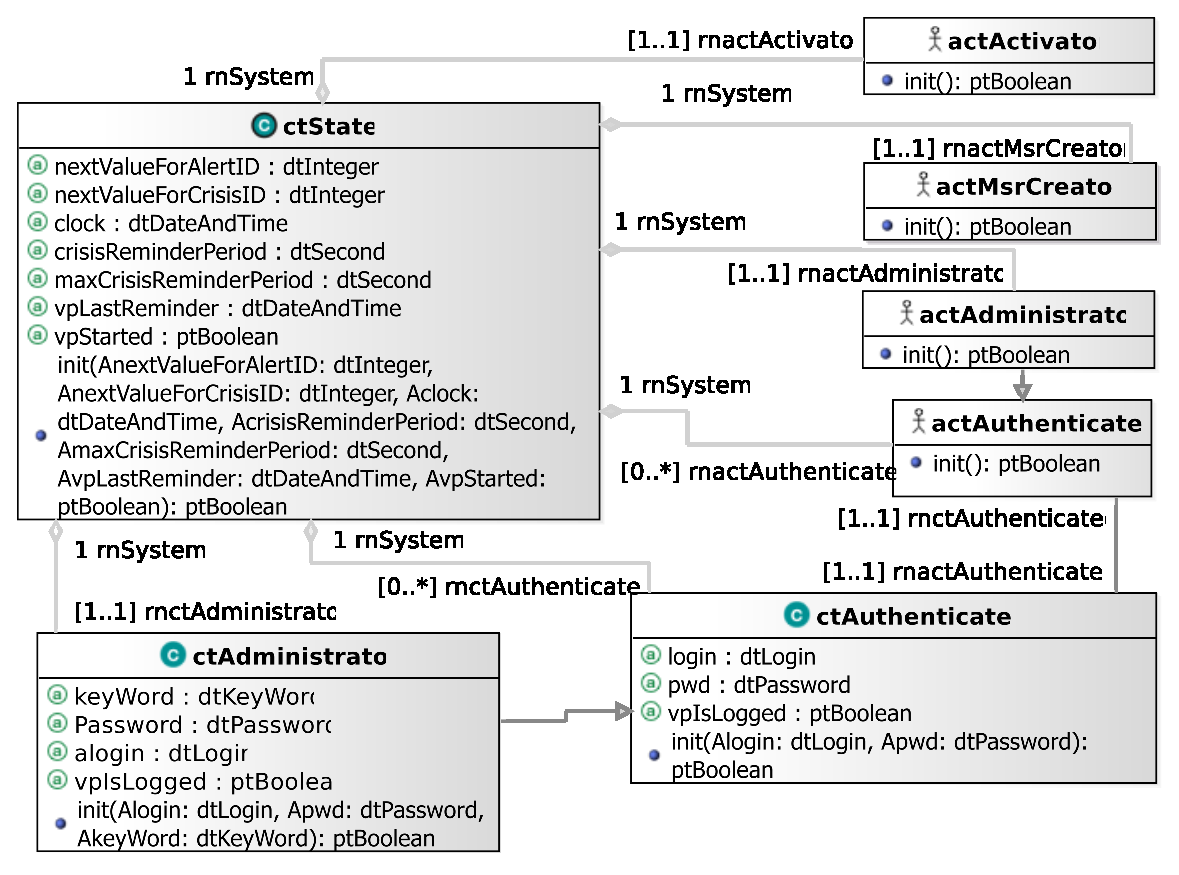
\includegraphics[
angle=0
,width=1.0\textwidth
]{./images-report-gen/operation-model/operation-scope-outactMsrCreator-oeCreateSystemAndEnvironment.eps}
\end{center}
\caption[lu.uni.lassy.excalibur.examples.icrash Operation Scope: operation-scope-outactMsrCreator-oeCreateSystemAndEnvironment]{oeCreateSystemAndEnvironment operation scope
}
\label{fig:lu.uni.lassy.excalibur.examples.icrash-OM-scopeView-operation-scope-outactMsrCreator-oeCreateSystemAndEnvironment}
\end{figure}
\vspace{0.5cm}



%% ***************************************************************
%% operations for: Environment-Actor Operation Schemes

		
\section{Environment - Actor Operation Scheme for actMsrCreator}
\label{OM-EM-actMsrCreator}
\subsection{Operation Model for init}

\label{OM-init}


The \msrcode{init} operation has the following properties:

	\begin{operationmodel}
	\addheading{Operation}
	\adddoublerow{init}{used to create an instance of the actor together with its interface instances and update the assocations with the \msrcode{ctState} instance.}


	\addrowheading{Return type}
	\addsinglerow{ptBoolean}

		


	\end{operationmodel}



	
	
	
	





 

%% ***************************************************************
%% operations for primary type classes


\section{Primary Types - Operation Schemes for Class ctAdministrator} 
\label{OM-CM-PTClass-ctAdministrator}
\subsection{Operation Model for init}

\label{OM-init}


The \msrcode{init} operation has the following properties:

	\begin{operationmodel}
	\addheading{Operation}
	\adddoublerow{init}{ used to initialize the current object as a new instance of the ctAdministrator type.}

	\addrowheading{Parameters}
	\addnumbereddoublerow{}{Alogin: dtLogin}{used to initialize the login field} 
	\addnumbereddoublerow{}{Apwd: dtPassword}{used to initialize the password field} 

	\addrowheading{Return type}
	\addsinglerow{ptBoolean}

		

	\addrowheading{Post-Condition (functional)}
	\addnumberedsinglerow{PostF}{ 
	true iff the system poststate includes the current object as a new ctAdministrator instance having its login and password attributes equal to the one provided as parameters and its vpIsLogged attribute equal to false. }

	\end{operationmodel}



	% ------------------------------------------
	% MCL Listing
	% ------------------------------------------
	\vspace{1cm}
	The listing~\ref{OM-ctAdministrator-init-MCL-LST} provides the \msrmessir (MCL-oriented) specification of the operation.
	
	\scriptsize
	\vspace{0.5cm}
	\begin{lstlisting}[style=MessirStyle,firstnumber=auto,captionpos=b,caption={\msrmessir (MCL-oriented) specification of the operation \emph{init}.},label=OM-ctAdministrator-init-MCL-LST]

	
	
	/* Post Functional:*/ 
	postF{if
	(
	let Self:ctAdministrator in
	/* Post F01 */
	Self.login(Alogin)
	and Self.pwd = Apwd
	and Self.vpIsLogged = false
	
	/* Post F02 */
	and (Self.oclIsNew and self = Self)
	)
	then (result = true)
	else (result = false)
	endif}
	
	
	\end{lstlisting}
	\normalsize 
	
	
	
	
	% ------------------------------------------
	% PROLOG Listing
	% ------------------------------------------
	
	\vspace{1cm}
	The listing~\ref{OM-ctAdministrator-init-PROLOG-LST} provides the \msrmessir (Prolog-oriented) implementation of the operation.
	
	\scriptsize
	\vspace{0.5cm}
	
	\lstinputlisting[style=MessirPrologStyle,firstnumber=auto,captionpos=b,caption={\msrmessir (Prolog-oriented) implementation of the operation \emph{init}.},label=OM-ctAdministrator-init-PROLOG-LST]{../lu.uni.lassy.excalibur.examples.icrash.simulation/src/Operations/Concepts/PrimaryTypesClasses/PrimaryTypesClasses-ctAdministrator-init.pl}
	\normalsize






\section{Primary Types - Operation Schemes for Class ctAlert} 
\label{OM-CM-PTClass-ctAlert}
\subsection{Operation Model for init}

\label{OM-init}


The \msrcode{init} operation has the following properties:

	\begin{operationmodel}
	\addheading{Operation}
	\adddoublerow{init}{ used to initialize the current object as a new instance of the ctAlert type.}

	\addrowheading{Parameters}
	\addnumbereddoublerow{}{Aid: dtAlertID}{used to initialize the id field} 
	\addnumbereddoublerow{}{Astatus: etAlertStatus}{used to initialize the status field} 
	\addnumbereddoublerow{}{Alocation: dtGPSLocation}{used to initialize the location field} 
	\addnumbereddoublerow{}{Ainstant: dtDateAndTime}{used to initialize the instant field} 
	\addnumbereddoublerow{}{Acomment: dtComment}{used to initialize the comment field} 

	\addrowheading{Return type}
	\addsinglerow{ptBoolean}

		

	\addrowheading{Post-Condition (functional)}
	\addnumberedsinglerow{PostF}{true iff the system poststate includes the current object as a new ctAlert instance having its attributes equal to the ones provided as parameters. 
	}

	\end{operationmodel}



	% ------------------------------------------
	% MCL Listing
	% ------------------------------------------
	\vspace{1cm}
	The listing~\ref{OM-ctAlert-init-MCL-LST} provides the \msrmessir (MCL-oriented) specification of the operation.
	
	\scriptsize
	\vspace{0.5cm}
	\begin{lstlisting}[style=MessirStyle,firstnumber=auto,captionpos=b,caption={\msrmessir (MCL-oriented) specification of the operation \emph{init}.},label=OM-ctAlert-init-MCL-LST]

	
	
	/* Post Functional:*/ 
	postF{if
	(
	/* Post F01 */
	let Self:ctAlert in
	Self.id = Aid
	and Self.status = Astatus
	and Self.location = Alocation
	and Self.instant = Ainstant
	and Self.comment = Acomment
	/* Post F02 */
	and (Self.oclIsNew and self = Self)
	)
	then (result = true)
	else (result = false)
	endif}
	
	
	\end{lstlisting}
	\normalsize 
	
	
	
	
	% ------------------------------------------
	% PROLOG Listing
	% ------------------------------------------
	
	\vspace{1cm}
	The listing~\ref{OM-ctAlert-init-PROLOG-LST} provides the \msrmessir (Prolog-oriented) implementation of the operation.
	
	\scriptsize
	\vspace{0.5cm}
	
	\lstinputlisting[style=MessirPrologStyle,firstnumber=auto,captionpos=b,caption={\msrmessir (Prolog-oriented) implementation of the operation \emph{init}.},label=OM-ctAlert-init-PROLOG-LST]{../lu.uni.lassy.excalibur.examples.icrash.simulation/src/Operations/Concepts/PrimaryTypesClasses/PrimaryTypesClasses-ctAlert-init.pl}
	\normalsize






\subsection{Operation Model for isSentToCoordinator}

\label{OM-isSentToCoordinator}


The \msrcode{isSentToCoordinator} operation has the following properties:

	\begin{operationmodel}
	\addheading{Operation}
	\adddoublerow{isSentToCoordinator}{ used to provide a given coordinator with current alert information.}

	\addrowheading{Parameters}
	\addnumbereddoublerow{}{AactCoordinator: actCoordinator}{the message destination} 

	\addrowheading{Return type}
	\addsinglerow{ptBoolean}

		

	\addrowheading{Post-Condition (functional)}
	\addnumberedsinglerow{PostF}{ true iff the message ieSendAnAlert is sent to the input interface of the given coordinator actor with the current alert as parameter value.}

	\end{operationmodel}



	% ------------------------------------------
	% MCL Listing
	% ------------------------------------------
	\vspace{1cm}
	The listing~\ref{OM-ctAlert-isSentToCoordinator-MCL-LST} provides the \msrmessir (MCL-oriented) specification of the operation.
	
	\scriptsize
	\vspace{0.5cm}
	\begin{lstlisting}[style=MessirStyle,firstnumber=auto,captionpos=b,caption={\msrmessir (MCL-oriented) specification of the operation \emph{isSentToCoordinator}.},label=OM-ctAlert-isSentToCoordinator-MCL-LST]

	
	
	/* Post Functional:*/ 
	postF{if
	(
	/* Post F01 */
	AactCoordinator.rnInterfaceIN.ieSendAnAlert(self)
	)
	then (result = true)
	else (result = false)
	endif}
	
	
	\end{lstlisting}
	\normalsize 
	
	
	
	
	% ------------------------------------------
	% PROLOG Listing
	% ------------------------------------------
	
	\vspace{1cm}
	The listing~\ref{OM-ctAlert-isSentToCoordinator-PROLOG-LST} provides the \msrmessir (Prolog-oriented) implementation of the operation.
	
	\scriptsize
	\vspace{0.5cm}
	
	\lstinputlisting[style=MessirPrologStyle,firstnumber=auto,captionpos=b,caption={\msrmessir (Prolog-oriented) implementation of the operation \emph{isSentToCoordinator}.},label=OM-ctAlert-isSentToCoordinator-PROLOG-LST]{../lu.uni.lassy.excalibur.examples.icrash.simulation/src/Operations/Concepts/PrimaryTypesClasses/PrimaryTypesClasses-ctAlert-isSentToCoordinator.pl}
	\normalsize






\section{Primary Types - Operation Schemes for Class ctAuthenticated} 
\label{OM-CM-PTClass-ctAuthenticated}
\subsection{Operation Model for init}

\label{OM-init}


The \msrcode{init} operation has the following properties:

	\begin{operationmodel}
	\addheading{Operation}
	\adddoublerow{init}{used to initialize the current object as a new instance of the ctAuthenticated type.}

	\addrowheading{Parameters}
	\addnumbereddoublerow{}{Alogin: dtLogin}{used to initialize the login field} 
	\addnumbereddoublerow{}{Apwd: dtPassword}{used to initialize the password field} 

	\addrowheading{Return type}
	\addsinglerow{ptBoolean}

		

	\addrowheading{Post-Condition (functional)}
	\addnumberedsinglerow{PostF}{true iff the system poststate includes the current object as a new ctAuthenticated instance having its attributes equal to the ones provided as parameters.}

	\end{operationmodel}



	
	
	
	
	% ------------------------------------------
	% PROLOG Listing
	% ------------------------------------------
	
	\vspace{1cm}
	The listing~\ref{OM-ctAuthenticated-init-PROLOG-LST} provides the \msrmessir (Prolog-oriented) implementation of the operation.
	
	\scriptsize
	\vspace{0.5cm}
	
	\lstinputlisting[style=MessirPrologStyle,firstnumber=auto,captionpos=b,caption={\msrmessir (Prolog-oriented) implementation of the operation \emph{init}.},label=OM-ctAuthenticated-init-PROLOG-LST]{../lu.uni.lassy.excalibur.examples.icrash.simulation/src/Operations/Concepts/PrimaryTypesClasses/PrimaryTypesClasses-ctAuthenticated-init.pl}
	\normalsize






\section{Primary Types - Operation Schemes for Class ctCoordinator} 
\label{OM-CM-PTClass-ctCoordinator}
\subsection{Operation Model for init}

\label{OM-init}


The \msrcode{init} operation has the following properties:

	\begin{operationmodel}
	\addheading{Operation}
	\adddoublerow{init}{used to initialize the current object as a new instance of the ctCoordinator type.}

	\addrowheading{Parameters}
	\addnumbereddoublerow{}{Aid: dtCoordinatorID}{used to initialize the id field} 
	\addnumbereddoublerow{}{Alogin: dtLogin}{used to initialize the login field} 
	\addnumbereddoublerow{}{Apwd: dtPassword}{used to initialize the password field} 

	\addrowheading{Return type}
	\addsinglerow{ptBoolean}

		

	\addrowheading{Post-Condition (functional)}
	\addnumberedsinglerow{PostF}{true iff the system poststate includes the current object as a new ctCoordinator instance having its attributes equal to the ones provided as parameters.
	 }

	\end{operationmodel}



	% ------------------------------------------
	% MCL Listing
	% ------------------------------------------
	\vspace{1cm}
	The listing~\ref{OM-ctCoordinator-init-MCL-LST} provides the \msrmessir (MCL-oriented) specification of the operation.
	
	\scriptsize
	\vspace{0.5cm}
	\begin{lstlisting}[style=MessirStyle,firstnumber=auto,captionpos=b,caption={\msrmessir (MCL-oriented) specification of the operation \emph{init}.},label=OM-ctCoordinator-init-MCL-LST]

	
	
	/* Post Functional:*/ 
	postF{if
	(
	/* Post F01 */
	let Self:ctCoordinator in
	Self.id = Aid
	and Self.login = Alogin
	and Self.pwd = Apwd
	and Self.vpIsLogged = false
	/* Post F02 */
	and (Self.oclIsNew and self = Self)
	)
	then (result = true)
	else (result = false)
	endif}
	
	
	\end{lstlisting}
	\normalsize 
	
	
	
	
	% ------------------------------------------
	% PROLOG Listing
	% ------------------------------------------
	
	\vspace{1cm}
	The listing~\ref{OM-ctCoordinator-init-PROLOG-LST} provides the \msrmessir (Prolog-oriented) implementation of the operation.
	
	\scriptsize
	\vspace{0.5cm}
	
	\lstinputlisting[style=MessirPrologStyle,firstnumber=auto,captionpos=b,caption={\msrmessir (Prolog-oriented) implementation of the operation \emph{init}.},label=OM-ctCoordinator-init-PROLOG-LST]{../lu.uni.lassy.excalibur.examples.icrash.simulation/src/Operations/Concepts/PrimaryTypesClasses/PrimaryTypesClasses-ctCoordinator-init.pl}
	\normalsize






\section{Primary Types - Operation Schemes for Class ctCrisis} 
\label{OM-CM-PTClass-ctCrisis}
\subsection{Operation Model for init}

\label{OM-init}


The \msrcode{init} operation has the following properties:

	\begin{operationmodel}
	\addheading{Operation}
	\adddoublerow{init}{ used to initialize the current object as a new instance of the ctCrisis type.}

	\addrowheading{Parameters}
	\addnumbereddoublerow{}{Aid: dtCrisisID}{used to initialize the id field} 
	\addnumbereddoublerow{}{Atype: etCrisisType}{used to initialize the type field} 
	\addnumbereddoublerow{}{Astatus: etCrisisStatus}{used to initialize the status field} 
	\addnumbereddoublerow{}{Alocation: dtGPSLocation}{used to initialize the location field} 
	\addnumbereddoublerow{}{Ainstant: dtDateAndTime}{used to initialize the instant field} 
	\addnumbereddoublerow{}{Acomment: dtComment}{used to initialize the comment field} 
	\addnumbereddoublerow{}{Adeadline: dtDateAndTime}{used to initialize the deadline field} 
	\addnumbereddoublerow{}{Aremain: dtDateAndTime}{used to initialize the remain field} 
	\addnumbereddoublerow{}{Apasstime: dtDateAndTime}{used to initialize the passtime field} 

	\addrowheading{Return type}
	\addsinglerow{ptBoolean}

		

	\addrowheading{Post-Condition (functional)}
	\addnumberedsinglerow{PostF}{true iff the system poststate includes the current object as a new ctCrisis instance having its attributes equal to the ones provided as parameters.
	}

	\end{operationmodel}



	% ------------------------------------------
	% MCL Listing
	% ------------------------------------------
	\vspace{1cm}
	The listing~\ref{OM-ctCrisis-init-MCL-LST} provides the \msrmessir (MCL-oriented) specification of the operation.
	
	\scriptsize
	\vspace{0.5cm}
	\begin{lstlisting}[style=MessirStyle,firstnumber=auto,captionpos=b,caption={\msrmessir (MCL-oriented) specification of the operation \emph{init}.},label=OM-ctCrisis-init-MCL-LST]

	
	
	/* Post Functional:*/ 
	postF{if
	(
	/* Post F01 */
	let Self:ctCrisis in
	Self.id = Aid
	and Self.type = Atype
	and Self.status = Astatus
	and Self.location = Alocation
	and Self.instant = Ainstant
	and Self.comment = Acomment
	and Self.deadline = Adeadline
	and Self.remain = Aremain
	and Self.passtime = Apasstime
	/* Post F02 */
	and (Self.oclIsNew and self = Self)
	)
	then (result = true)
	else (result = false)
	endif}
	
	
	\end{lstlisting}
	\normalsize 
	
	
	
	
	% ------------------------------------------
	% PROLOG Listing
	% ------------------------------------------
	
	\vspace{1cm}
	The listing~\ref{OM-ctCrisis-init-PROLOG-LST} provides the \msrmessir (Prolog-oriented) implementation of the operation.
	
	\scriptsize
	\vspace{0.5cm}
	
	\lstinputlisting[style=MessirPrologStyle,firstnumber=auto,captionpos=b,caption={\msrmessir (Prolog-oriented) implementation of the operation \emph{init}.},label=OM-ctCrisis-init-PROLOG-LST]{../lu.uni.lassy.excalibur.examples.icrash.simulation/src/Operations/Concepts/PrimaryTypesClasses/PrimaryTypesClasses-ctCrisis-init.pl}
	\normalsize






\subsection{Operation Model for handlingDelayPassed}

\label{OM-handlingDelayPassed}


The \msrcode{handlingDelayPassed} operation has the following properties:

	\begin{operationmodel}
	\addheading{Operation}
	\adddoublerow{handlingDelayPassed}{used to determine if the crisis stood too longly in a pending status since last reminder.}


	\addrowheading{Return type}
	\addsinglerow{ptBoolean}

		

	\addrowheading{Post-Condition (functional)}
	\addnumberedsinglerow{PostF}{true iff the crisis is in pending status and if the duration between the current ctState clock information and the last reminder is greater than the crisis reminder period duration.}

	\end{operationmodel}



	% ------------------------------------------
	% MCL Listing
	% ------------------------------------------
	\vspace{1cm}
	The listing~\ref{OM-ctCrisis-handlingDelayPassed-MCL-LST} provides the \msrmessir (MCL-oriented) specification of the operation.
	
	\scriptsize
	\vspace{0.5cm}
	\begin{lstlisting}[style=MessirStyle,firstnumber=auto,captionpos=b,caption={\msrmessir (MCL-oriented) specification of the operation \emph{handlingDelayPassed}.},label=OM-ctCrisis-handlingDelayPassed-MCL-LST]

	
	
	/* Post Functional:*/ 
	postF{let TheSystem:ctState in
	let CurrentClockSecondsQty:dtInteger in
	let vpLastReminderSecondsQty:dtInteger in
	let CrisisReminderPeriod:dtSecond in
	if 
	( /* Post F01 */
	  self.rnSystem = TheSystem
	  and self.status = pending
	  and TheSystem.clock.toSecondsQty() = CurrentClockSecondsQty
	  and TheSystem.vpLastReminder.toSecondsQty() = vpLastReminderSecondsQty
	  and TheSystem.crisisReminderPeriod = CrisisReminderPeriod
	  and CurrentClockSecondsQty.sub(vpLastReminderSecondsQty).gt(CrisisReminderPeriod) = true
	)
	then (result = true)
	else (result = false)
	endif}
	
	
	\end{lstlisting}
	\normalsize 
	
	
	
	
	% ------------------------------------------
	% PROLOG Listing
	% ------------------------------------------
	
	\vspace{1cm}
	The listing~\ref{OM-ctCrisis-handlingDelayPassed-PROLOG-LST} provides the \msrmessir (Prolog-oriented) implementation of the operation.
	
	\scriptsize
	\vspace{0.5cm}
	
	\lstinputlisting[style=MessirPrologStyle,firstnumber=auto,captionpos=b,caption={\msrmessir (Prolog-oriented) implementation of the operation \emph{handlingDelayPassed}.},label=OM-ctCrisis-handlingDelayPassed-PROLOG-LST]{../lu.uni.lassy.excalibur.examples.icrash.simulation/src/Operations/Concepts/PrimaryTypesClasses/PrimaryTypesClasses-ctCrisis-handlingDelayPassed.pl}
	\normalsize






\subsection{Operation Model for maxHandlingDelayPassed}

\label{OM-maxHandlingDelayPassed}


The \msrcode{maxHandlingDelayPassed} operation has the following properties:

	\begin{operationmodel}
	\addheading{Operation}
	\adddoublerow{maxHandlingDelayPassed}{used to determine if the crisis stood too longly in a pending status since its creation.}


	\addrowheading{Return type}
	\addsinglerow{ptBoolean}

		

	\addrowheading{Post-Condition (functional)}
	\addnumberedsinglerow{PostF}{ true iff the crisis is in pending status and if the duration between the current ctState clock information and the crisis instant is greater than the maximum reminder period duration.}

	\end{operationmodel}



	% ------------------------------------------
	% MCL Listing
	% ------------------------------------------
	\vspace{1cm}
	The listing~\ref{OM-ctCrisis-maxHandlingDelayPassed-MCL-LST} provides the \msrmessir (MCL-oriented) specification of the operation.
	
	\scriptsize
	\vspace{0.5cm}
	\begin{lstlisting}[style=MessirStyle,firstnumber=auto,captionpos=b,caption={\msrmessir (MCL-oriented) specification of the operation \emph{maxHandlingDelayPassed}.},label=OM-ctCrisis-maxHandlingDelayPassed-MCL-LST]

	
	
	/* Post Functional:*/ 
	postF{let TheSystem:ctState in
	let CurrentClockSecondsQty:dtInteger in
	let CrisisInstantSecondsQty:dtInteger in
	let MaxCrisisReminderPeriod:dtSecond in
	if 
	( /* Post F01 */
	  self.rnSystem = TheSystem
	  and self.status = pending
	  and TheSystem.clock.toSecondsQty() = CurrentClockSecondsQty
	  and Self.instant.toSecondsQty() = CrisisInstantSecondsQty
	  and TheSystem.maxCrisisReminderPeriod = MaxCrisisReminderPeriod
	  and CurrentClockSecondsQty.sub(CrisisInstantSecondsQty)
	                            .gt(MaxCrisisReminderPeriod)
	)
	then (result = true)
	else (result = false)
	endif}
	
	
	\end{lstlisting}
	\normalsize 
	
	
	
	
	% ------------------------------------------
	% PROLOG Listing
	% ------------------------------------------
	
	\vspace{1cm}
	The listing~\ref{OM-ctCrisis-maxHandlingDelayPassed-PROLOG-LST} provides the \msrmessir (Prolog-oriented) implementation of the operation.
	
	\scriptsize
	\vspace{0.5cm}
	
	\lstinputlisting[style=MessirPrologStyle,firstnumber=auto,captionpos=b,caption={\msrmessir (Prolog-oriented) implementation of the operation \emph{maxHandlingDelayPassed}.},label=OM-ctCrisis-maxHandlingDelayPassed-PROLOG-LST]{../lu.uni.lassy.excalibur.examples.icrash.simulation/src/Operations/Concepts/PrimaryTypesClasses/PrimaryTypesClasses-ctCrisis-maxHandlingDelayPassed.pl}
	\normalsize






\subsection{Operation Model for isSentToCoordinator}

\label{OM-isSentToCoordinator}


The \msrcode{isSentToCoordinator} operation has the following properties:

	\begin{operationmodel}
	\addheading{Operation}
	\adddoublerow{isSentToCoordinator}{used to provide a given coordinator with current crisis information.}

	\addrowheading{Parameters}
	\addnumbereddoublerow{}{AactCoordinator: actCoordinator}{the message destination actor} 

	\addrowheading{Return type}
	\addsinglerow{ptBoolean}

		

	\addrowheading{Post-Condition (functional)}
	\addnumberedsinglerow{PostF}{ true iff the message ieSendACrisis is sent by the simulator to the input interface of the given coordinator actor with the current crisis as parameter value.
	}

	\end{operationmodel}



	% ------------------------------------------
	% MCL Listing
	% ------------------------------------------
	\vspace{1cm}
	The listing~\ref{OM-ctCrisis-isSentToCoordinator-MCL-LST} provides the \msrmessir (MCL-oriented) specification of the operation.
	
	\scriptsize
	\vspace{0.5cm}
	\begin{lstlisting}[style=MessirStyle,firstnumber=auto,captionpos=b,caption={\msrmessir (MCL-oriented) specification of the operation \emph{isSentToCoordinator}.},label=OM-ctCrisis-isSentToCoordinator-MCL-LST]

	
	
	/* Post Functional:*/ 
	postF{if 
	(
	/* Post F01 */
	  AactCoordinator.rnInterfaceIN.ieSendACrisis(self)
	)
	then (result = true)
	else (result = false)
	endif}
	
	
	\end{lstlisting}
	\normalsize 
	
	
	
	
	% ------------------------------------------
	% PROLOG Listing
	% ------------------------------------------
	
	\vspace{1cm}
	The listing~\ref{OM-ctCrisis-isSentToCoordinator-PROLOG-LST} provides the \msrmessir (Prolog-oriented) implementation of the operation.
	
	\scriptsize
	\vspace{0.5cm}
	
	\lstinputlisting[style=MessirPrologStyle,firstnumber=auto,captionpos=b,caption={\msrmessir (Prolog-oriented) implementation of the operation \emph{isSentToCoordinator}.},label=OM-ctCrisis-isSentToCoordinator-PROLOG-LST]{../lu.uni.lassy.excalibur.examples.icrash.simulation/src/Operations/Concepts/PrimaryTypesClasses/PrimaryTypesClasses-ctCrisis-isSentToCoordinator.pl}
	\normalsize






\subsection{Operation Model for isAllocatedIfPossible}

\label{OM-isAllocatedIfPossible}


The \msrcode{isAllocatedIfPossible} operation has the following properties:

	\begin{operationmodel}
	\addheading{Operation}
	\adddoublerow{isAllocatedIfPossible}{used to allocate a crisis to a coordinator if any or to alert the administrator of crisis waiting to be handled.}


	\addrowheading{Return type}
	\addsinglerow{ptBoolean}

		

	\addrowheading{Post-Condition (functional)}
	\addnumberedsinglerow{PostF}{ true iff the duration between the crisis creation and the system's clock is greater than the maximum delay defined
	and }
	\addnumberedsinglerow{PostF}{if there exist at least one coordinator then (a) the post state associates to the crisis any of the existing coordinators and (b) the coordinator is informed that he is now the handlers of the crisis whose ID is communicated}
	\addnumberedsinglerow{PostF}{else a message is sent to all known administrators to request creation of new coordinators.}

	\end{operationmodel}



	% ------------------------------------------
	% MCL Listing
	% ------------------------------------------
	\vspace{1cm}
	The listing~\ref{OM-ctCrisis-isAllocatedIfPossible-MCL-LST} provides the \msrmessir (MCL-oriented) specification of the operation.
	
	\scriptsize
	\vspace{0.5cm}
	\begin{lstlisting}[style=MessirStyle,firstnumber=auto,captionpos=b,caption={\msrmessir (MCL-oriented) specification of the operation \emph{isAllocatedIfPossible}.},label=OM-ctCrisis-isAllocatedIfPossible-MCL-LST]

	
	
	/* Post Functional:*/ 
	postF{if (   
	/* Post F01 */
	self.maxHandlingDelayPassed()
	and 
	  if  (TheSystem.rnactCoordinator->msrIsEmpty = false)
	  then (
	      /* Post F02 */
	      TheSystem.rnactCoordinator->msrAny(true) = TheCoordinatorActor
	      and TheCoordinatorActor.rnctCoordinator = TheCoordinator
	      and self@post.rnHandler = TheCoordinator
	      and self@post.status = handled
	      and self.id.value = TheCrisisIDptString
	      and 'You are now considered as handling the crisis having ID: '
	          .ptStringConcat(TheCrisisIDptString) = TheMessage
	        and TheCoordinatorActor.rnInterfaceIN^ieMessage(TheMessage)
	   )
	  else (  /* Post F03 */
	        TheSystem.rnactAdministrator
	        ->forAll(rnInterfaceIN.ieMessage('Please add new coordinators to handle pending crisis !'))
	    )
	  endif
	  )
	then (result = true)
	else (result = false)
	endif}
	
	
	\end{lstlisting}
	\normalsize 
	
	
	
	
	% ------------------------------------------
	% PROLOG Listing
	% ------------------------------------------
	
	\vspace{1cm}
	The listing~\ref{OM-ctCrisis-isAllocatedIfPossible-PROLOG-LST} provides the \msrmessir (Prolog-oriented) implementation of the operation.
	
	\scriptsize
	\vspace{0.5cm}
	
	\lstinputlisting[style=MessirPrologStyle,firstnumber=auto,captionpos=b,caption={\msrmessir (Prolog-oriented) implementation of the operation \emph{isAllocatedIfPossible}.},label=OM-ctCrisis-isAllocatedIfPossible-PROLOG-LST]{../lu.uni.lassy.excalibur.examples.icrash.simulation/src/Operations/Concepts/PrimaryTypesClasses/PrimaryTypesClasses-ctCrisis-isAllocatedIfPossible.pl}
	\normalsize






\section{Primary Types - Operation Schemes for Class ctHuman} 
\label{OM-CM-PTClass-ctHuman}
\subsection{Operation Model for init}

\label{OM-init}


The \msrcode{init} operation has the following properties:

	\begin{operationmodel}
	\addheading{Operation}
	\adddoublerow{init}{used to initialize the current object as a new instance of the ctHuman type.}

	\addrowheading{Parameters}
	\addnumbereddoublerow{}{Aid: dtPhoneNumber}{used to initialize the id field} 
	\addnumbereddoublerow{}{Akind: etHumanKind}{used to initialize the kind field} 

	\addrowheading{Return type}
	\addsinglerow{ptBoolean}

		

	\addrowheading{Post-Condition (functional)}
	\addnumberedsinglerow{PostF}{true iff the system poststate includes the current object as a new ctHuman instance having its attributes equal to the ones provided as parameters.
	}

	\end{operationmodel}



	% ------------------------------------------
	% MCL Listing
	% ------------------------------------------
	\vspace{1cm}
	The listing~\ref{OM-ctHuman-init-MCL-LST} provides the \msrmessir (MCL-oriented) specification of the operation.
	
	\scriptsize
	\vspace{0.5cm}
	\begin{lstlisting}[style=MessirStyle,firstnumber=auto,captionpos=b,caption={\msrmessir (MCL-oriented) specification of the operation \emph{init}.},label=OM-ctHuman-init-MCL-LST]

	
	
	/* Post Functional:*/ 
	postF{if
	(
	/* Post F01 */
	let Self:ctHuman in
	
	Self.id = Aid
	and Self.kind = Akind
	
	/* Post F02 */
	and (Self.oclIsNew and self = Self)
	)
	then (result = true)
	else (result = false)
	endif}
	
	
	\end{lstlisting}
	\normalsize 
	
	
	
	
	% ------------------------------------------
	% PROLOG Listing
	% ------------------------------------------
	
	\vspace{1cm}
	The listing~\ref{OM-ctHuman-init-PROLOG-LST} provides the \msrmessir (Prolog-oriented) implementation of the operation.
	
	\scriptsize
	\vspace{0.5cm}
	
	\lstinputlisting[style=MessirPrologStyle,firstnumber=auto,captionpos=b,caption={\msrmessir (Prolog-oriented) implementation of the operation \emph{init}.},label=OM-ctHuman-init-PROLOG-LST]{../lu.uni.lassy.excalibur.examples.icrash.simulation/src/Operations/Concepts/PrimaryTypesClasses/PrimaryTypesClasses-ctHuman-init.pl}
	\normalsize






\subsection{Operation Model for isAcknowledged}

\label{OM-isAcknowledged}


The \msrcode{isAcknowledged} operation has the following properties:

	\begin{operationmodel}
	\addheading{Operation}
	\adddoublerow{isAcknowledged}{ used to specify the property of having sent an alert acknowledge message to the human having declared the alert through its own communication company.}


	\addrowheading{Return type}
	\addsinglerow{ptBoolean}

		

	\addrowheading{Post-Condition (functional)}
	\addnumberedsinglerow{PostF}{
	true iff the message ieSmsSend is sent to the related input interface of the related communication company actor with the human phone number and the generic message 'The handling of your alert by our services is in progress !'
	}

	\end{operationmodel}



	
	
	
	
	% ------------------------------------------
	% PROLOG Listing
	% ------------------------------------------
	
	\vspace{1cm}
	The listing~\ref{OM-ctHuman-isAcknowledged-PROLOG-LST} provides the \msrmessir (Prolog-oriented) implementation of the operation.
	
	\scriptsize
	\vspace{0.5cm}
	
	\lstinputlisting[style=MessirPrologStyle,firstnumber=auto,captionpos=b,caption={\msrmessir (Prolog-oriented) implementation of the operation \emph{isAcknowledged}.},label=OM-ctHuman-isAcknowledged-PROLOG-LST]{../lu.uni.lassy.excalibur.examples.icrash.simulation/src/Operations/Concepts/PrimaryTypesClasses/PrimaryTypesClasses-ctHuman-isAcknowledged.pl}
	\normalsize






\section{Primary Types - Operation Schemes for Class ctState} 
\label{OM-CM-PTClass-ctState}
\subsection{Operation Model for init}

\label{OM-init}


The \msrcode{init} operation has the following properties:

	\begin{operationmodel}
	\addheading{Operation}
	\adddoublerow{init}{ used to initialize the current object as a new instance of the ctState type.}

	\addrowheading{Parameters}
	\addnumbereddoublerow{}{AnextValueForAlertID: dtInteger}{used to initialize the nextValueForAlertID field} 
	\addnumbereddoublerow{}{AnextValueForCrisisID: dtInteger}{used to initialize the nextValueForCrisisID field} 
	\addnumbereddoublerow{}{Aclock: dtDateAndTime}{used to initialize the clock field} 
	\addnumbereddoublerow{}{AcrisisReminderPeriod: dtSecond}{used to initialize the crisisReminderPeriod field} 
	\addnumbereddoublerow{}{AmaxCrisisReminderPeriod: dtSecond}{used to initialize the maxCrisisReminderPeriod field} 
	\addnumbereddoublerow{}{AvpLastReminder: dtDateAndTime}{used to initialize the vpLastReminder field} 
	\addnumbereddoublerow{}{AvpStarted: ptBoolean}{used to initialize the vpStarted field} 

	\addrowheading{Return type}
	\addsinglerow{ptBoolean}

		

	\addrowheading{Post-Condition (functional)}
	\addnumberedsinglerow{PostF}{ 
	true iff the system poststate includes the current object as a new ctState instance having its attributes equal to the ones provided as parameters. 
	}

	\end{operationmodel}



	% ------------------------------------------
	% MCL Listing
	% ------------------------------------------
	\vspace{1cm}
	The listing~\ref{OM-ctState-init-MCL-LST} provides the \msrmessir (MCL-oriented) specification of the operation.
	
	\scriptsize
	\vspace{0.5cm}
	\begin{lstlisting}[style=MessirStyle,firstnumber=auto,captionpos=b,caption={\msrmessir (MCL-oriented) specification of the operation \emph{init}.},label=OM-ctState-init-MCL-LST]

	
	
	/* Post Functional:*/ 
	postF{if
	(
	/* Post F01 */
	let Self:ctState in
	
	Self.nextValueForAlertID = AnextValueForAlertID
	and Self.nextValueForCrisisID = AnextValueForCrisisID
	and Self.clock = Aclock
	and Self.crisisReminderPeriod = AcrisisReminderPeriod
	and Self.maxCrisisReminderPeriod = AmaxCrisisReminderPeriod
	and Self.vpLastReminder = AvpLastReminder
	and Self.vpStarted = AvpStarted
	
	and (Self.oclIsNew and self = Self)
	)
	then (result = true)
	else (result = false)
	endif}
	
	
	\end{lstlisting}
	\normalsize 
	
	
	
	
	% ------------------------------------------
	% PROLOG Listing
	% ------------------------------------------
	
	\vspace{1cm}
	The listing~\ref{OM-ctState-init-PROLOG-LST} provides the \msrmessir (Prolog-oriented) implementation of the operation.
	
	\scriptsize
	\vspace{0.5cm}
	
	\lstinputlisting[style=MessirPrologStyle,firstnumber=auto,captionpos=b,caption={\msrmessir (Prolog-oriented) implementation of the operation \emph{init}.},label=OM-ctState-init-PROLOG-LST]{../lu.uni.lassy.excalibur.examples.icrash.simulation/src/Operations/Concepts/PrimaryTypesClasses/PrimaryTypesClasses-ctState-init.pl}
	\normalsize








%% ***************************************************************
%% operations for primary type datatypes and enumerations



\section{Primary Types - Operation Schemes for Datatype dtAlertID} 
\label{OM-CM-PTDataType-dtAlertID}
\subsection{Operation Model for is}

\label{OM-is}


The \msrcode{is} operation has the following properties:

	\begin{operationmodel}
	\addheading{Operation}
	\adddoublerow{is}{ used to determine which strings are considered as valid alert identifiers.}


	\addrowheading{Return type}
	\addsinglerow{ptBoolean}

		

	\addrowheading{Post-Condition (functional)}
	\addnumberedsinglerow{PostF}{ if the length of the value attribute of a dtAlertID is a ptInteger greater than zero 
	and lower or equal to 20 then the operation returns the ptBoolean true, else the ptBoolean false.}

	\end{operationmodel}



	% ------------------------------------------
	% MCL Listing
	% ------------------------------------------
	\vspace{1cm}
	The listing~\ref{OM-dtAlertID-is-MCL-LST} provides the \msrmessir (MCL-oriented) specification of the operation.
	
	\scriptsize
	\vspace{0.5cm}
	\begin{lstlisting}[style=MessirStyle,firstnumber=auto,captionpos=b,caption={\msrmessir (MCL-oriented) specification of the operation \emph{is}.},label=OM-dtAlertID-is-MCL-LST]

	
	
	/* Post Functional:*/ 
	postF{let TheResult: ptBoolean in
	    ( if
	      ( AdtValue.value.length().gt(0)
	        and AdtValue.value.length().leq(20)
	      )
	      then (TheResult = true)
	      else (TheResult = false)
	      endif
	      result = TheResult
	    )}
	
	
	\end{lstlisting}
	\normalsize 
	
	
	
	
	% ------------------------------------------
	% PROLOG Listing
	% ------------------------------------------
	
	\vspace{1cm}
	The listing~\ref{OM-dtAlertID-is-PROLOG-LST} provides the \msrmessir (Prolog-oriented) implementation of the operation.
	
	\scriptsize
	\vspace{0.5cm}
	
	\lstinputlisting[style=MessirPrologStyle,firstnumber=auto,captionpos=b,caption={\msrmessir (Prolog-oriented) implementation of the operation \emph{is}.},label=OM-dtAlertID-is-PROLOG-LST]{../lu.uni.lassy.excalibur.examples.icrash.simulation/src/Operations/Concepts/PrimaryTypesDatatypes/PrimaryTypesDatatypes-dtAlertID-is.pl}
	\normalsize






\section{Primary Types - Operation Schemes for Datatype dtComment} 
\label{OM-CM-PTDataType-dtComment}
\subsection{Operation Model for is}

\label{OM-is}


The \msrcode{is} operation has the following properties:

	\begin{operationmodel}
	\addheading{Operation}
	\adddoublerow{is}{used to determine which strings are considered as valid comments.}


	\addrowheading{Return type}
	\addsinglerow{ptBoolean}

		

	\addrowheading{Post-Condition (functional)}
	\addnumberedsinglerow{PostF}{true iff the length of the string value is not more than 160 characters.}

	\end{operationmodel}



	% ------------------------------------------
	% MCL Listing
	% ------------------------------------------
	\vspace{1cm}
	The listing~\ref{OM-dtComment-is-MCL-LST} provides the \msrmessir (MCL-oriented) specification of the operation.
	
	\scriptsize
	\vspace{0.5cm}
	\begin{lstlisting}[style=MessirStyle,firstnumber=auto,captionpos=b,caption={\msrmessir (MCL-oriented) specification of the operation \emph{is}.},label=OM-dtComment-is-MCL-LST]

	
	
	/* Post Functional:*/ 
	postF{let TheResult: ptBoolean in
	        ( if
	          ( MaxLength = 160
	            and AdtValue.value.length().leq(MaxLength)
	          )
	          then (TheResult = true)
	          else (TheResult = false)
	          endif
	          result = TheResult
	        )}
	
	
	\end{lstlisting}
	\normalsize 
	
	
	
	
	% ------------------------------------------
	% PROLOG Listing
	% ------------------------------------------
	
	\vspace{1cm}
	The listing~\ref{OM-dtComment-is-PROLOG-LST} provides the \msrmessir (Prolog-oriented) implementation of the operation.
	
	\scriptsize
	\vspace{0.5cm}
	
	\lstinputlisting[style=MessirPrologStyle,firstnumber=auto,captionpos=b,caption={\msrmessir (Prolog-oriented) implementation of the operation \emph{is}.},label=OM-dtComment-is-PROLOG-LST]{../lu.uni.lassy.excalibur.examples.icrash.simulation/src/Operations/Concepts/PrimaryTypesDatatypes/PrimaryTypesDatatypes-dtComment-is.pl}
	\normalsize






\section{Primary Types - Operation Schemes for Datatype dtCoordinatorID} 
\label{OM-CM-PTDataType-dtCoordinatorID}
\subsection{Operation Model for is}

\label{OM-is}


The \msrcode{is} operation has the following properties:

	\begin{operationmodel}
	\addheading{Operation}
	\adddoublerow{is}{used to determine which string are considered as valid alert identifiers.}


	\addrowheading{Return type}
	\addsinglerow{ptBoolean}

		

	\addrowheading{Post-Condition (functional)}
	\addnumberedsinglerow{PostF}{ if the length of the value attribute of a dtCoordinatorID is a ptInteger greater than zero 
	and lower or equal to 5 than the operation returns the ptBoolean true, else the ptBoolean false.}

	\end{operationmodel}



	% ------------------------------------------
	% MCL Listing
	% ------------------------------------------
	\vspace{1cm}
	The listing~\ref{OM-dtCoordinatorID-is-MCL-LST} provides the \msrmessir (MCL-oriented) specification of the operation.
	
	\scriptsize
	\vspace{0.5cm}
	\begin{lstlisting}[style=MessirStyle,firstnumber=auto,captionpos=b,caption={\msrmessir (MCL-oriented) specification of the operation \emph{is}.},label=OM-dtCoordinatorID-is-MCL-LST]

	
	
	/* Post Functional:*/ 
	postF{let TheResult: ptBoolean in
	        ( if
	          ( AdtValue.value.length().gt(0)
	            and AdtValue.value.length().leq(5)
	          )
	          then (TheResult = true)
	          else (TheResult = false)
	          endif
	          result = TheResult
	        )}
	
	
	\end{lstlisting}
	\normalsize 
	
	
	
	
	% ------------------------------------------
	% PROLOG Listing
	% ------------------------------------------
	
	\vspace{1cm}
	The listing~\ref{OM-dtCoordinatorID-is-PROLOG-LST} provides the \msrmessir (Prolog-oriented) implementation of the operation.
	
	\scriptsize
	\vspace{0.5cm}
	
	\lstinputlisting[style=MessirPrologStyle,firstnumber=auto,captionpos=b,caption={\msrmessir (Prolog-oriented) implementation of the operation \emph{is}.},label=OM-dtCoordinatorID-is-PROLOG-LST]{../lu.uni.lassy.excalibur.examples.icrash.simulation/src/Operations/Concepts/PrimaryTypesDatatypes/PrimaryTypesDatatypes-dtCoordinatorID-is.pl}
	\normalsize






\section{Primary Types - Operation Schemes for Datatype dtCrisisID} 
\label{OM-CM-PTDataType-dtCrisisID}
\subsection{Operation Model for is}

\label{OM-is}


The \msrcode{is} operation has the following properties:

	\begin{operationmodel}
	\addheading{Operation}
	\adddoublerow{is}{ used to determine which strings are considered as valid crisis identifiers.}


	\addrowheading{Return type}
	\addsinglerow{ptBoolean}

		

	\addrowheading{Post-Condition (functional)}
	\addnumberedsinglerow{PostF}{ if the length of the value attribute of a dtCrisisID is a ptInteger greater than zero 
	and lower or equal to 10 than the operation returns the ptBoolean true, else the ptBoolean false.}

	\end{operationmodel}



	% ------------------------------------------
	% MCL Listing
	% ------------------------------------------
	\vspace{1cm}
	The listing~\ref{OM-dtCrisisID-is-MCL-LST} provides the \msrmessir (MCL-oriented) specification of the operation.
	
	\scriptsize
	\vspace{0.5cm}
	\begin{lstlisting}[style=MessirStyle,firstnumber=auto,captionpos=b,caption={\msrmessir (MCL-oriented) specification of the operation \emph{is}.},label=OM-dtCrisisID-is-MCL-LST]

	
	
	/* Post Functional:*/ 
	postF{let TheResult: ptBoolean in
	        ( if
	          ( AdtValue.value.length().gt(0)
	            and AdtValue.value.length().leq(10)
	          )
	          then (TheResult = true)
	          else (TheResult = false)
	          endif
	          result = TheResult
	        )}
	
	
	\end{lstlisting}
	\normalsize 
	
	
	
	
	% ------------------------------------------
	% PROLOG Listing
	% ------------------------------------------
	
	\vspace{1cm}
	The listing~\ref{OM-dtCrisisID-is-PROLOG-LST} provides the \msrmessir (Prolog-oriented) implementation of the operation.
	
	\scriptsize
	\vspace{0.5cm}
	
	\lstinputlisting[style=MessirPrologStyle,firstnumber=auto,captionpos=b,caption={\msrmessir (Prolog-oriented) implementation of the operation \emph{is}.},label=OM-dtCrisisID-is-PROLOG-LST]{../lu.uni.lassy.excalibur.examples.icrash.simulation/src/Operations/Concepts/PrimaryTypesDatatypes/PrimaryTypesDatatypes-dtCrisisID-is.pl}
	\normalsize






\section{Primary Types - Operation Schemes for Datatype dtGPSLocation} 
\label{OM-CM-PTDataType-dtGPSLocation}
\subsection{Operation Model for is}

\label{OM-is}


The \msrcode{is} operation has the following properties:

	\begin{operationmodel}
	\addheading{Operation}
	\adddoublerow{is}{used to determine which couples are considered as valid dtGPSLocation values.}


	\addrowheading{Return type}
	\addsinglerow{ptBoolean}

		

	\addrowheading{Post-Condition (functional)}
	\addnumberedsinglerow{PostF}{ true if both latitude and longitude are valid values according to their is operation.}

	\end{operationmodel}



	% ------------------------------------------
	% MCL Listing
	% ------------------------------------------
	\vspace{1cm}
	The listing~\ref{OM-dtGPSLocation-is-MCL-LST} provides the \msrmessir (MCL-oriented) specification of the operation.
	
	\scriptsize
	\vspace{0.5cm}
	\begin{lstlisting}[style=MessirStyle,firstnumber=auto,captionpos=b,caption={\msrmessir (MCL-oriented) specification of the operation \emph{is}.},label=OM-dtGPSLocation-is-MCL-LST]

	
	
	/* Post Functional:*/ 
	postF{let TheResult: ptBoolean in
	        ( if
	          ( AdtValue.latitude.is()
	            and AdtValue.longitude.is
	          )
	          then (TheResult = true)
	          else (TheResult = false)
	          endif
	          result = TheResult
	        )}
	
	
	\end{lstlisting}
	\normalsize 
	
	
	
	
	% ------------------------------------------
	% PROLOG Listing
	% ------------------------------------------
	
	\vspace{1cm}
	The listing~\ref{OM-dtGPSLocation-is-PROLOG-LST} provides the \msrmessir (Prolog-oriented) implementation of the operation.
	
	\scriptsize
	\vspace{0.5cm}
	
	\lstinputlisting[style=MessirPrologStyle,firstnumber=auto,captionpos=b,caption={\msrmessir (Prolog-oriented) implementation of the operation \emph{is}.},label=OM-dtGPSLocation-is-PROLOG-LST]{../lu.uni.lassy.excalibur.examples.icrash.simulation/src/Operations/Concepts/PrimaryTypesDatatypes/PrimaryTypesDatatypes-dtGPSLocation-is.pl}
	\normalsize






\subsection{Operation Model for isNearTo}

\label{OM-isNearTo}


The \msrcode{isNearTo} operation has the following properties:

	\begin{operationmodel}
	\addheading{Operation}
	\adddoublerow{isNearTo}{used to determine if locations are considered enough close to be treated as equivalent in the application domain context. In the context of the iCrash system, we compute the distance between two GPS locations using the following Haversine formula.
	(more details can be found at: 
	  http://www.movable-type.co.uk/scripts/latlong.html
	  and http://www.gpsvisualizer.com/calculators\#distance
	)
	 }

	\addrowheading{Parameters}
	\addnumbereddoublerow{}{AGPSLocation: dtGPSLocation}{the GPS location to be compared to.} 

	\addrowheading{Return type}
	\addsinglerow{ptBoolean}

		

	\addrowheading{Post-Condition (functional)}
	\addnumberedsinglerow{PostF}{ if the Haversine formula (ACOS(SIN(lat1)*SIN(lat2)+COS(lat1)*COS(lat2)*COS(lon2-lon1))*6371, in which latitudes and longitudes are in radiansapplied to the two dtGPS coordinates is lower to 100 meters)
	then the predicate is true and false otherwise.}

	\end{operationmodel}



	% ------------------------------------------
	% MCL Listing
	% ------------------------------------------
	\vspace{1cm}
	The listing~\ref{OM-dtGPSLocation-isNearTo-MCL-LST} provides the \msrmessir (MCL-oriented) specification of the operation.
	
	\scriptsize
	\vspace{0.5cm}
	\begin{lstlisting}[style=MessirStyle,firstnumber=auto,captionpos=b,caption={\msrmessir (MCL-oriented) specification of the operation \emph{isNearTo}.},label=OM-dtGPSLocation-isNearTo-MCL-LST]

	
	
	/* Post Functional:*/ 
	postF{let TheResult: ptBoolean in true
	        let EarthRadius: dtReal in
	        let MaxDistance: dtReal in
	        let ComparedLatitude: dtLatitude in
	        let ComparedLongitude: dtLongitude in
	        let R1: dtReal in let R1a: dtReal in
	        let R2: dtReal in let R2a: dtReal in
	        
	        ( if
	          ( EarthRadius.value = 6371
	            and MaxDistance.value = 100
	            
	            and AdtValue.latitude = ComparedLatitude
	            and AdtValue.longitude = ComparedLongitude
	            and Self.latitude.sin() = R1a
	            and AdtValue.latitude.sin().mul(R1a) = R1
	            and Self.latitude.cos() = R2a
	            and AdtValue.latitude.cos().mul(R2a) = R2
	            
	            and AdtValue.longitude = ComparedLongitude
	            and Self.longitude.sub(ComparedLongitude).cos().mul(R2)
	                    .add(R1).acos().mul(EarthRadius).sub(MaxDistance)
	                    .value.leq(0)
	          )
	          then (TheResult = true)
	          else (TheResult = false)
	          endif
	          result = TheResult
	        )}
	
	
	\end{lstlisting}
	\normalsize 
	
	
	
	
	% ------------------------------------------
	% PROLOG Listing
	% ------------------------------------------
	
	\vspace{1cm}
	The listing~\ref{OM-dtGPSLocation-isNearTo-PROLOG-LST} provides the \msrmessir (Prolog-oriented) implementation of the operation.
	
	\scriptsize
	\vspace{0.5cm}
	
	\lstinputlisting[style=MessirPrologStyle,firstnumber=auto,captionpos=b,caption={\msrmessir (Prolog-oriented) implementation of the operation \emph{isNearTo}.},label=OM-dtGPSLocation-isNearTo-PROLOG-LST]{../lu.uni.lassy.excalibur.examples.icrash.simulation/src/Operations/Concepts/PrimaryTypesDatatypes/PrimaryTypesDatatypes-dtGPSLocation-isNearTo.pl}
	\normalsize






\section{Primary Types - Operation Schemes for Datatype dtKeyWord} 
\label{OM-CM-PTDataType-dtKeyWord}
\subsection{Operation Model for is}

\label{OM-is}


The \msrcode{is} operation has the following properties:

	\begin{operationmodel}
	\addheading{Operation}
	\adddoublerow{is}{ used to determine which strings are considered as valid dtKeyWord.}


	\addrowheading{Return type}
	\addsinglerow{ptBoolean}

		

	\addrowheading{Post-Condition (functional)}
	\addnumberedsinglerow{PostF}{is true of the length of the string value is at least 6 characters long.}

	\end{operationmodel}



	% ------------------------------------------
	% MCL Listing
	% ------------------------------------------
	\vspace{1cm}
	The listing~\ref{OM-dtKeyWord-is-MCL-LST} provides the \msrmessir (MCL-oriented) specification of the operation.
	
	\scriptsize
	\vspace{0.5cm}
	\begin{lstlisting}[style=MessirStyle,firstnumber=auto,captionpos=b,caption={\msrmessir (MCL-oriented) specification of the operation \emph{is}.},label=OM-dtKeyWord-is-MCL-LST]

	
	
	/* Post Functional:*/ 
	postF{let TheResult: ptBoolean in
	        let MinLength: ptInteger in
	        ( if
	          ( MinLength = 6
	            and AdtValue.value.length().geq(MinLength)
	          )
	          then (TheResult = true)
	          else (TheResult = false)
	          endif
	          result = TheResult
	        )}
	
	
	\end{lstlisting}
	\normalsize 
	
	
	
	






\section{Primary Types - Operation Schemes for Datatype dtLatitude} 
\label{OM-CM-PTDataType-dtLatitude}
\subsection{Operation Model for is}

\label{OM-is}


The \msrcode{is} operation has the following properties:

	\begin{operationmodel}
	\addheading{Operation}
	\adddoublerow{is}{used to determine which strings are considered as valid dtLatitude.}


	\addrowheading{Return type}
	\addsinglerow{ptBoolean}

		

	\addrowheading{Post-Condition (functional)}
	\addnumberedsinglerow{PostF}{ is true if the value is a real in the interval [-90.0 , +90.0].}

	\end{operationmodel}



	% ------------------------------------------
	% MCL Listing
	% ------------------------------------------
	\vspace{1cm}
	The listing~\ref{OM-dtLatitude-is-MCL-LST} provides the \msrmessir (MCL-oriented) specification of the operation.
	
	\scriptsize
	\vspace{0.5cm}
	\begin{lstlisting}[style=MessirStyle,firstnumber=auto,captionpos=b,caption={\msrmessir (MCL-oriented) specification of the operation \emph{is}.},label=OM-dtLatitude-is-MCL-LST]

	
	
	/* Post Functional:*/ 
	postF{let TheResult: ptBoolean in
	        ( if
	          ( AdtValue.value.geq(-90.0)
	            and AdtValue.value.leq(+90.0)
	          )
	          then (TheResult = true)
	          else (TheResult = false)
	          endif
	          result = TheResult
	        )}
	
	
	\end{lstlisting}
	\normalsize 
	
	
	
	
	% ------------------------------------------
	% PROLOG Listing
	% ------------------------------------------
	
	\vspace{1cm}
	The listing~\ref{OM-dtLatitude-is-PROLOG-LST} provides the \msrmessir (Prolog-oriented) implementation of the operation.
	
	\scriptsize
	\vspace{0.5cm}
	
	\lstinputlisting[style=MessirPrologStyle,firstnumber=auto,captionpos=b,caption={\msrmessir (Prolog-oriented) implementation of the operation \emph{is}.},label=OM-dtLatitude-is-PROLOG-LST]{../lu.uni.lassy.excalibur.examples.icrash.simulation/src/Operations/Concepts/PrimaryTypesDatatypes/PrimaryTypesDatatypes-dtLatitude-is.pl}
	\normalsize






\section{Primary Types - Operation Schemes for Datatype dtLogin} 
\label{OM-CM-PTDataType-dtLogin}
\subsection{Operation Model for is}

\label{OM-is}


The \msrcode{is} operation has the following properties:

	\begin{operationmodel}
	\addheading{Operation}
	\adddoublerow{is}{ used to determine which strings are considered as valid dtLogin.}


	\addrowheading{Return type}
	\addsinglerow{ptBoolean}

		

	\addrowheading{Post-Condition (functional)}
	\addnumberedsinglerow{PostF}{is true of the length of the string value is not more than 20 characters.}

	\end{operationmodel}



	% ------------------------------------------
	% MCL Listing
	% ------------------------------------------
	\vspace{1cm}
	The listing~\ref{OM-dtLogin-is-MCL-LST} provides the \msrmessir (MCL-oriented) specification of the operation.
	
	\scriptsize
	\vspace{0.5cm}
	\begin{lstlisting}[style=MessirStyle,firstnumber=auto,captionpos=b,caption={\msrmessir (MCL-oriented) specification of the operation \emph{is}.},label=OM-dtLogin-is-MCL-LST]

	
	
	/* Post Functional:*/ 
	postF{let TheResult: ptBoolean in
	        let MaxLength: ptInteger in
	        ( if
	          ( MaxLength = 20
	            and AdtValue.value.length().leq(MaxLength)
	          )
	          then (TheResult = true)
	          else (TheResult = false)
	          endif
	          result = TheResult
	        )}
	
	
	\end{lstlisting}
	\normalsize 
	
	
	
	
	% ------------------------------------------
	% PROLOG Listing
	% ------------------------------------------
	
	\vspace{1cm}
	The listing~\ref{OM-dtLogin-is-PROLOG-LST} provides the \msrmessir (Prolog-oriented) implementation of the operation.
	
	\scriptsize
	\vspace{0.5cm}
	
	\lstinputlisting[style=MessirPrologStyle,firstnumber=auto,captionpos=b,caption={\msrmessir (Prolog-oriented) implementation of the operation \emph{is}.},label=OM-dtLogin-is-PROLOG-LST]{../lu.uni.lassy.excalibur.examples.icrash.simulation/src/Operations/Concepts/PrimaryTypesDatatypes/PrimaryTypesDatatypes-dtLogin-is.pl}
	\normalsize






\section{Primary Types - Operation Schemes for Datatype dtLongitude} 
\label{OM-CM-PTDataType-dtLongitude}
\subsection{Operation Model for is}

\label{OM-is}


The \msrcode{is} operation has the following properties:

	\begin{operationmodel}
	\addheading{Operation}
	\adddoublerow{is}{used to determine which strings are considered as valid dtLongitude.}


	\addrowheading{Return type}
	\addsinglerow{ptBoolean}

		

	\addrowheading{Post-Condition (functional)}
	\addnumberedsinglerow{PostF}{ is true if the value is a real in the interval [-180.0 , +180.0].}

	\end{operationmodel}



	% ------------------------------------------
	% MCL Listing
	% ------------------------------------------
	\vspace{1cm}
	The listing~\ref{OM-dtLongitude-is-MCL-LST} provides the \msrmessir (MCL-oriented) specification of the operation.
	
	\scriptsize
	\vspace{0.5cm}
	\begin{lstlisting}[style=MessirStyle,firstnumber=auto,captionpos=b,caption={\msrmessir (MCL-oriented) specification of the operation \emph{is}.},label=OM-dtLongitude-is-MCL-LST]

	
	
	/* Post Functional:*/ 
	postF{let TheResult: ptBoolean in
	        ( if
	          ( AdtValue.value.geq(-180.0)
	            and AdtValue.value.leq(+180.0)
	          )
	          then (TheResult = true)
	          else (TheResult = false)
	          endif
	          result = TheResult
	        )}
	
	
	\end{lstlisting}
	\normalsize 
	
	
	
	
	% ------------------------------------------
	% PROLOG Listing
	% ------------------------------------------
	
	\vspace{1cm}
	The listing~\ref{OM-dtLongitude-is-PROLOG-LST} provides the \msrmessir (Prolog-oriented) implementation of the operation.
	
	\scriptsize
	\vspace{0.5cm}
	
	\lstinputlisting[style=MessirPrologStyle,firstnumber=auto,captionpos=b,caption={\msrmessir (Prolog-oriented) implementation of the operation \emph{is}.},label=OM-dtLongitude-is-PROLOG-LST]{../lu.uni.lassy.excalibur.examples.icrash.simulation/src/Operations/Concepts/PrimaryTypesDatatypes/PrimaryTypesDatatypes-dtLongitude-is.pl}
	\normalsize






\section{Primary Types - Operation Schemes for Datatype dtPassword} 
\label{OM-CM-PTDataType-dtPassword}
\subsection{Operation Model for is}

\label{OM-is}


The \msrcode{is} operation has the following properties:

	\begin{operationmodel}
	\addheading{Operation}
	\adddoublerow{is}{ used to determine which strings are considered as valid dtPassword.}


	\addrowheading{Return type}
	\addsinglerow{ptBoolean}

		

	\addrowheading{Post-Condition (functional)}
	\addnumberedsinglerow{PostF}{is true of the length of the string value is at least 6 characters long.}

	\end{operationmodel}



	% ------------------------------------------
	% MCL Listing
	% ------------------------------------------
	\vspace{1cm}
	The listing~\ref{OM-dtPassword-is-MCL-LST} provides the \msrmessir (MCL-oriented) specification of the operation.
	
	\scriptsize
	\vspace{0.5cm}
	\begin{lstlisting}[style=MessirStyle,firstnumber=auto,captionpos=b,caption={\msrmessir (MCL-oriented) specification of the operation \emph{is}.},label=OM-dtPassword-is-MCL-LST]

	
	
	/* Post Functional:*/ 
	postF{let TheResult: ptBoolean in
	        let MinLength: ptInteger in
	        ( if
	          ( MinLength = 6
	            and AdtValue.value.length().geq(MinLength)
	          )
	          then (TheResult = true)
	          else (TheResult = false)
	          endif
	          result = TheResult
	        )}
	
	
	\end{lstlisting}
	\normalsize 
	
	
	
	
	% ------------------------------------------
	% PROLOG Listing
	% ------------------------------------------
	
	\vspace{1cm}
	The listing~\ref{OM-dtPassword-is-PROLOG-LST} provides the \msrmessir (Prolog-oriented) implementation of the operation.
	
	\scriptsize
	\vspace{0.5cm}
	
	\lstinputlisting[style=MessirPrologStyle,firstnumber=auto,captionpos=b,caption={\msrmessir (Prolog-oriented) implementation of the operation \emph{is}.},label=OM-dtPassword-is-PROLOG-LST]{../lu.uni.lassy.excalibur.examples.icrash.simulation/src/Operations/Concepts/PrimaryTypesDatatypes/PrimaryTypesDatatypes-dtPassword-is.pl}
	\normalsize






\section{Primary Types - Operation Schemes for Datatype dtPhoneNumber} 
\label{OM-CM-PTDataType-dtPhoneNumber}
\subsection{Operation Model for is}

\label{OM-is}


The \msrcode{is} operation has the following properties:

	\begin{operationmodel}
	\addheading{Operation}
	\adddoublerow{is}{used to determine which strings are considered as valid dtPhoneNumber.}


	\addrowheading{Return type}
	\addsinglerow{ptBoolean}

		

	\addrowheading{Post-Condition (functional)}
	\addnumberedsinglerow{PostF}{is true of the length of the string value is from 4 to 30 characters. No standard is applied !}

	\end{operationmodel}



	% ------------------------------------------
	% MCL Listing
	% ------------------------------------------
	\vspace{1cm}
	The listing~\ref{OM-dtPhoneNumber-is-MCL-LST} provides the \msrmessir (MCL-oriented) specification of the operation.
	
	\scriptsize
	\vspace{0.5cm}
	\begin{lstlisting}[style=MessirStyle,firstnumber=auto,captionpos=b,caption={\msrmessir (MCL-oriented) specification of the operation \emph{is}.},label=OM-dtPhoneNumber-is-MCL-LST]

	
	
	/* Post Functional:*/ 
	postF{let TheResult: ptBoolean in
	    ( if
	      ( AdtValue.value.length().gt(4)
	        and AdtValue.value.length().leq(30)
	      )
	      then (TheResult = true)
	      else (TheResult = false)
	      endif
	      result = TheResult
	    )}
	
	
	\end{lstlisting}
	\normalsize 
	
	
	
	
	% ------------------------------------------
	% PROLOG Listing
	% ------------------------------------------
	
	\vspace{1cm}
	The listing~\ref{OM-dtPhoneNumber-is-PROLOG-LST} provides the \msrmessir (Prolog-oriented) implementation of the operation.
	
	\scriptsize
	\vspace{0.5cm}
	
	\lstinputlisting[style=MessirPrologStyle,firstnumber=auto,captionpos=b,caption={\msrmessir (Prolog-oriented) implementation of the operation \emph{is}.},label=OM-dtPhoneNumber-is-PROLOG-LST]{../lu.uni.lassy.excalibur.examples.icrash.simulation/src/Operations/Concepts/PrimaryTypesDatatypes/PrimaryTypesDatatypes-dtPhoneNumber-is.pl}
	\normalsize










\section{Primary Types - Operation Schemes for Enumeration etAlertStatus} 
\label{OM-CM-PTEnumType-etAlertStatus}
\subsection{Operation Model for is}

\label{OM-is}


The \msrcode{is} operation has the following properties:

	\begin{operationmodel}
	\addheading{Operation}
	\adddoublerow{is}{ used to determine which litteral belongs to the enumeration.}


	\addrowheading{Return type}
	\addsinglerow{ptBoolean}

		

	\addrowheading{Post-Condition (functional)}
	\addnumberedsinglerow{PostF}{true iff the value is equal to one of the following values: \msrcode{pending, valid, invalid}}

	\end{operationmodel}



	% ------------------------------------------
	% MCL Listing
	% ------------------------------------------
	\vspace{1cm}
	The listing~\ref{OM-etAlertStatus-is-MCL-LST} provides the \msrmessir (MCL-oriented) specification of the operation.
	
	\scriptsize
	\vspace{0.5cm}
	\begin{lstlisting}[style=MessirStyle,firstnumber=auto,captionpos=b,caption={\msrmessir (MCL-oriented) specification of the operation \emph{is}.},label=OM-etAlertStatus-is-MCL-LST]

	
	
	/* Post Functional:*/ 
	postF{let TheResult: ptBoolean in
	        ( if
	          ( self = pending
	            or self = valid
	            or self = invalid
	          )
	          then (TheResult = true)
	          else (TheResult = false)
	          endif
	          result = TheResult
	        )}
	
	
	\end{lstlisting}
	\normalsize 
	
	
	
	
	% ------------------------------------------
	% PROLOG Listing
	% ------------------------------------------
	
	\vspace{1cm}
	The listing~\ref{OM-etAlertStatus-is-PROLOG-LST} provides the \msrmessir (Prolog-oriented) implementation of the operation.
	
	\scriptsize
	\vspace{0.5cm}
	
	\lstinputlisting[style=MessirPrologStyle,firstnumber=auto,captionpos=b,caption={\msrmessir (Prolog-oriented) implementation of the operation \emph{is}.},label=OM-etAlertStatus-is-PROLOG-LST]{../lu.uni.lassy.excalibur.examples.icrash.simulation/src/Operations/Concepts/PrimaryTypesClasses/PrimaryTypesDatatypes-etAlertStatus-is.pl}
	\normalsize






\section{Primary Types - Operation Schemes for Enumeration etCrisisStatus} 
\label{OM-CM-PTEnumType-etCrisisStatus}
\subsection{Operation Model for is}

\label{OM-is}


The \msrcode{is} operation has the following properties:

	\begin{operationmodel}
	\addheading{Operation}
	\adddoublerow{is}{used to determine which litteral belongs to the enumeration.}


	\addrowheading{Return type}
	\addsinglerow{ptBoolean}

		

	\addrowheading{Post-Condition (functional)}
	\addnumberedsinglerow{PostF}{true iff the value is equal to one of the following values: \msrcode{pending, handled, solved, closed}.}

	\end{operationmodel}



	% ------------------------------------------
	% MCL Listing
	% ------------------------------------------
	\vspace{1cm}
	The listing~\ref{OM-etCrisisStatus-is-MCL-LST} provides the \msrmessir (MCL-oriented) specification of the operation.
	
	\scriptsize
	\vspace{0.5cm}
	\begin{lstlisting}[style=MessirStyle,firstnumber=auto,captionpos=b,caption={\msrmessir (MCL-oriented) specification of the operation \emph{is}.},label=OM-etCrisisStatus-is-MCL-LST]

	
	
	/* Post Functional:*/ 
	postF{let TheResult: ptBoolean in
	        ( if
	          ( self = pending
	            or self = handled
	            or self = solved
	            or self = closed
	          )
	          then (TheResult = true)
	          else (TheResult = false)
	          endif
	          result = TheResult
	        )}
	
	
	\end{lstlisting}
	\normalsize 
	
	
	
	
	% ------------------------------------------
	% PROLOG Listing
	% ------------------------------------------
	
	\vspace{1cm}
	The listing~\ref{OM-etCrisisStatus-is-PROLOG-LST} provides the \msrmessir (Prolog-oriented) implementation of the operation.
	
	\scriptsize
	\vspace{0.5cm}
	
	\lstinputlisting[style=MessirPrologStyle,firstnumber=auto,captionpos=b,caption={\msrmessir (Prolog-oriented) implementation of the operation \emph{is}.},label=OM-etCrisisStatus-is-PROLOG-LST]{../lu.uni.lassy.excalibur.examples.icrash.simulation/src/Operations/Concepts/PrimaryTypesClasses/PrimaryTypesDatatypes-etCrisisStatus-is.pl}
	\normalsize






\section{Primary Types - Operation Schemes for Enumeration etCrisisType} 
\label{OM-CM-PTEnumType-etCrisisType}
\subsection{Operation Model for is}

\label{OM-is}


The \msrcode{is} operation has the following properties:

	\begin{operationmodel}
	\addheading{Operation}
	\adddoublerow{is}{used to determine which litteral belongs to the enumeration. }


	\addrowheading{Return type}
	\addsinglerow{ptBoolean}

		

	\addrowheading{Post-Condition (functional)}
	\addnumberedsinglerow{PostF}{ true iff the value is equal to one of the following values: \msrcode{small, medium, huge}}

	\end{operationmodel}



	% ------------------------------------------
	% MCL Listing
	% ------------------------------------------
	\vspace{1cm}
	The listing~\ref{OM-etCrisisType-is-MCL-LST} provides the \msrmessir (MCL-oriented) specification of the operation.
	
	\scriptsize
	\vspace{0.5cm}
	\begin{lstlisting}[style=MessirStyle,firstnumber=auto,captionpos=b,caption={\msrmessir (MCL-oriented) specification of the operation \emph{is}.},label=OM-etCrisisType-is-MCL-LST]

	
	
	/* Post Functional:*/ 
	postF{let TheResult: ptBoolean in
	        ( if
	          ( self = small
	            or self = medium
	            or self = huge
	          )
	          then (TheResult = true)
	          else (TheResult = false)
	          endif
	          result = TheResult
	        )}
	
	
	\end{lstlisting}
	\normalsize 
	
	
	
	
	% ------------------------------------------
	% PROLOG Listing
	% ------------------------------------------
	
	\vspace{1cm}
	The listing~\ref{OM-etCrisisType-is-PROLOG-LST} provides the \msrmessir (Prolog-oriented) implementation of the operation.
	
	\scriptsize
	\vspace{0.5cm}
	
	\lstinputlisting[style=MessirPrologStyle,firstnumber=auto,captionpos=b,caption={\msrmessir (Prolog-oriented) implementation of the operation \emph{is}.},label=OM-etCrisisType-is-PROLOG-LST]{../lu.uni.lassy.excalibur.examples.icrash.simulation/src/Operations/Concepts/PrimaryTypesClasses/PrimaryTypesDatatypes-etCrisisType-is.pl}
	\normalsize






\section{Primary Types - Operation Schemes for Enumeration etHumanKind} 
\label{OM-CM-PTEnumType-etHumanKind}
\subsection{Operation Model for is}

\label{OM-is}


The \msrcode{is} operation has the following properties:

	\begin{operationmodel}
	\addheading{Operation}
	\adddoublerow{is}{ used to determine which litteral belongs to the enumeration.}


	\addrowheading{Return type}
	\addsinglerow{ptBoolean}

		

	\addrowheading{Post-Condition (functional)}
	\addnumberedsinglerow{PostF}{ true iff the value is equal to one of the following values: \msrcode{witness,victim,anonym}}

	\end{operationmodel}



	% ------------------------------------------
	% MCL Listing
	% ------------------------------------------
	\vspace{1cm}
	The listing~\ref{OM-etHumanKind-is-MCL-LST} provides the \msrmessir (MCL-oriented) specification of the operation.
	
	\scriptsize
	\vspace{0.5cm}
	\begin{lstlisting}[style=MessirStyle,firstnumber=auto,captionpos=b,caption={\msrmessir (MCL-oriented) specification of the operation \emph{is}.},label=OM-etHumanKind-is-MCL-LST]

	
	
	/* Post Functional:*/ 
	postF{let TheResult: ptBoolean in
	        ( if
	          ( self = witness
	            or self = victim
	            or self = anonymous
	          )
	          then (TheResult = true)
	          else (TheResult = false)
	          endif
	          result = TheResult
	        )}
	
	
	\end{lstlisting}
	\normalsize 
	
	
	
	
	% ------------------------------------------
	% PROLOG Listing
	% ------------------------------------------
	
	\vspace{1cm}
	The listing~\ref{OM-etHumanKind-is-PROLOG-LST} provides the \msrmessir (Prolog-oriented) implementation of the operation.
	
	\scriptsize
	\vspace{0.5cm}
	
	\lstinputlisting[style=MessirPrologStyle,firstnumber=auto,captionpos=b,caption={\msrmessir (Prolog-oriented) implementation of the operation \emph{is}.},label=OM-etHumanKind-is-PROLOG-LST]{../lu.uni.lassy.excalibur.examples.icrash.simulation/src/Operations/Concepts/PrimaryTypesClasses/PrimaryTypesDatatypes-etHumanKind-is.pl}
	\normalsize









%% ***************************************************************
%% operations for secondary type classes


\section{Secondary Types - Operation Schemes for Classes}
There are no elements in this category in the system analysed.




%% ***************************************************************
%% operations for secondary type datatypes and enumerations


\section{Secondary Types - Operation Schemes for Datatype dtSMS} 
\label{OM-CM-STDataType-dtSMS}
\subsection{Operation Model for is}

\label{OM-is}


The \msrcode{is} operation has the following properties:

	\begin{operationmodel}
	\addheading{Operation}
	\adddoublerow{is}{used to determine which strings are considered as valid comments}


	\addrowheading{Return type}
	\addsinglerow{ptBoolean}

		

	\addrowheading{Post-Condition (functional)}
	\addnumberedsinglerow{PostF}{true iff the length of the string value is not more than 160 characters.}

	\end{operationmodel}



	% ------------------------------------------
	% MCL Listing
	% ------------------------------------------
	\vspace{1cm}
	The listing~\ref{OM-dtSMS-is-MCL-LST} provides the \msrmessir (MCL-oriented) specification of the operation.
	
	\scriptsize
	\vspace{0.5cm}
	\begin{lstlisting}[style=MessirStyle,firstnumber=auto,captionpos=b,caption={\msrmessir (MCL-oriented) specification of the operation \emph{is}.},label=OM-dtSMS-is-MCL-LST]

	
	
	/* Post Functional:*/ 
	postF{let TheResult: ptBoolean in
	        let MaxLength: ptInteger in
	        ( if
	          ( MaxLength = 160
	            and AdtValue.value.length().leq(MaxLength)
	          )
	          then (TheResult = true)
	          else (TheResult = false)
	          endif
	          result = TheResult
	        )}
	
	
	\end{lstlisting}
	\normalsize 
	
	
	
	
	% ------------------------------------------
	% PROLOG Listing
	% ------------------------------------------
	
	\vspace{1cm}
	The listing~\ref{OM-dtSMS-is-PROLOG-LST} provides the \msrmessir (Prolog-oriented) implementation of the operation.
	
	\scriptsize
	\vspace{0.5cm}
	
	\lstinputlisting[style=MessirPrologStyle,firstnumber=auto,captionpos=b,caption={\msrmessir (Prolog-oriented) implementation of the operation \emph{is}.},label=OM-dtSMS-is-PROLOG-LST]{../lu.uni.lassy.excalibur.examples.icrash.simulation/src/Operations/Concepts/SecondaryTypesDatatypes/SecondaryTypesDatatypes-dtSMS-is.pl}
	\normalsize








\section{Secondary Types - Operation Schemes for Enumerations}
There are no elements in this category in the system analysed.




% doc-gen

% This is automatically generated and will be overwritten by the Generate Latex.


\newpage

% Last Modification:
% @author AUTHOR_NAME
% @date TODAY_DATE


\chapter{Additional Constraints}
\label{chap:additional_constraints}
\newpage

%APPENDICES
\appendix
% Last Modification:
% @author AUTHOR_NAME
% @date TODAY_DATE





		
\chapter{Undocumented Messir Specification Elements}











\section[Undocumented Primary Types]{Undocumented Primary Types}


\subsection[Undocumented Primary Datatype Types]{Undocumented Primary Datatype Types}
\begin{itemize}
\item lu.uni.lassy.messir.libraries.calendar.dtDate 
\item lu.uni.lassy.messir.libraries.calendar.dtDateAndTime 
\item lu.uni.lassy.messir.libraries.calendar.dtDay 
\item lu.uni.lassy.messir.libraries.calendar.dtHour 
\item lu.uni.lassy.messir.libraries.math.dtInteger 
\item lu.uni.lassy.messir.libraries.calendar.dtMinute 
\item lu.uni.lassy.messir.libraries.calendar.dtMonth 
\item lu.uni.lassy.messir.libraries.math.dtReal 
\item lu.uni.lassy.messir.libraries.calendar.dtSecond 
\item lu.uni.lassy.messir.libraries.string.dtString 
\item lu.uni.lassy.messir.libraries.calendar.dtTime 
\item lu.uni.lassy.messir.libraries.calendar.dtYear 
\end{itemize}



\subsection[Undocumented Primary Primitive Types]{Undocumented Primary Primitive Types}
\begin{itemize}
\item lu.uni.lassy.messir.libraries.primitives.ptBoolean 
\item lu.uni.lassy.messir.libraries.primitives.ptInteger 
\item lu.uni.lassy.messir.libraries.primitives.ptReal 
\item lu.uni.lassy.messir.libraries.primitives.ptString 
\end{itemize}













\section[Undocumented Operation Specifications]{Undocumented Operation Specifications}
\begin{itemize}
\item lu.uni.lassy.messir.libraries.calendar.dtDate.close 
\item lu.uni.lassy.messir.libraries.calendar.dtDate.eq 
\item lu.uni.lassy.messir.libraries.calendar.dtDate.fromSecondsQty 
\item lu.uni.lassy.messir.libraries.calendar.dtDate.gt 
\item lu.uni.lassy.messir.libraries.calendar.dtDate.is 
\item lu.uni.lassy.messir.libraries.calendar.dtDate.isNow 
\item lu.uni.lassy.messir.libraries.calendar.dtDate.lt 
\item lu.uni.lassy.messir.libraries.calendar.dtDate.toSecondsQty 
\item lu.uni.lassy.messir.libraries.calendar.dtDateAndTime.close 
\item lu.uni.lassy.messir.libraries.calendar.dtDateAndTime.eq 
\item lu.uni.lassy.messir.libraries.calendar.dtDateAndTime.fromSecondsQty 
\item lu.uni.lassy.messir.libraries.calendar.dtDateAndTime.gt 
\item lu.uni.lassy.messir.libraries.calendar.dtDateAndTime.is 
\item lu.uni.lassy.messir.libraries.calendar.dtDateAndTime.isNow 
\item lu.uni.lassy.messir.libraries.calendar.dtDateAndTime.lt 
\item lu.uni.lassy.messir.libraries.calendar.dtDateAndTime.toSecondsQty 
\item lu.uni.lassy.messir.libraries.calendar.dtDay.close 
\item lu.uni.lassy.messir.libraries.calendar.dtDay.is 
\item lu.uni.lassy.messir.libraries.calendar.dtHour.close 
\item lu.uni.lassy.messir.libraries.calendar.dtHour.is 
\item lu.uni.lassy.messir.libraries.math.dtInteger.acos 
\item lu.uni.lassy.messir.libraries.math.dtInteger.add 
\item lu.uni.lassy.messir.libraries.math.dtInteger.asdtReal 
\item lu.uni.lassy.messir.libraries.math.dtInteger.asin 
\item lu.uni.lassy.messir.libraries.math.dtInteger.asptInteger 
\item lu.uni.lassy.messir.libraries.math.dtInteger.atan 
\item lu.uni.lassy.messir.libraries.math.dtInteger.close 
\item lu.uni.lassy.messir.libraries.math.dtInteger.cos 
\item lu.uni.lassy.messir.libraries.math.dtInteger.eq 
\item lu.uni.lassy.messir.libraries.math.dtInteger.frac 
\item lu.uni.lassy.messir.libraries.math.dtInteger.geq 
\item lu.uni.lassy.messir.libraries.math.dtInteger.gt 
\item lu.uni.lassy.messir.libraries.math.dtInteger.is 
\item lu.uni.lassy.messir.libraries.math.dtInteger.leq 
\item lu.uni.lassy.messir.libraries.math.dtInteger.lt 
\item lu.uni.lassy.messir.libraries.math.dtInteger.mod 
\item lu.uni.lassy.messir.libraries.math.dtInteger.msrabs 
\item lu.uni.lassy.messir.libraries.math.dtInteger.msrdiv 
\item lu.uni.lassy.messir.libraries.math.dtInteger.mul 
\item lu.uni.lassy.messir.libraries.math.dtInteger.neq 
\item lu.uni.lassy.messir.libraries.math.dtInteger.opp 
\item lu.uni.lassy.messir.libraries.math.dtInteger.power 
\item lu.uni.lassy.messir.libraries.math.dtInteger.sin 
\item lu.uni.lassy.messir.libraries.math.dtInteger.sqr 
\item lu.uni.lassy.messir.libraries.math.dtInteger.sqrt 
\item lu.uni.lassy.messir.libraries.math.dtInteger.sub 
\item lu.uni.lassy.messir.libraries.math.dtInteger.tan 
\item lu.uni.lassy.messir.libraries.math.dtInteger.toDeg 
\item lu.uni.lassy.messir.libraries.math.dtInteger.toRad 
\item lu.uni.lassy.messir.libraries.math.dtInteger.todtString 
\item lu.uni.lassy.messir.libraries.calendar.dtMinute.close 
\item lu.uni.lassy.messir.libraries.calendar.dtMinute.is 
\item lu.uni.lassy.messir.libraries.calendar.dtMonth.close 
\item lu.uni.lassy.messir.libraries.calendar.dtMonth.is 
\item lu.uni.lassy.messir.libraries.math.dtReal.acos 
\item lu.uni.lassy.messir.libraries.math.dtReal.add 
\item lu.uni.lassy.messir.libraries.math.dtReal.asdtInteger 
\item lu.uni.lassy.messir.libraries.math.dtReal.asin 
\item lu.uni.lassy.messir.libraries.math.dtReal.asptReal 
\item lu.uni.lassy.messir.libraries.math.dtReal.atan 
\item lu.uni.lassy.messir.libraries.math.dtReal.close 
\item lu.uni.lassy.messir.libraries.math.dtReal.cos 
\item lu.uni.lassy.messir.libraries.math.dtReal.eq 
\item lu.uni.lassy.messir.libraries.math.dtReal.frac 
\item lu.uni.lassy.messir.libraries.math.dtReal.geq 
\item lu.uni.lassy.messir.libraries.math.dtReal.gt 
\item lu.uni.lassy.messir.libraries.math.dtReal.is 
\item lu.uni.lassy.messir.libraries.math.dtReal.leq 
\item lu.uni.lassy.messir.libraries.math.dtReal.lt 
\item lu.uni.lassy.messir.libraries.math.dtReal.msrabs 
\item lu.uni.lassy.messir.libraries.math.dtReal.msrdiv 
\item lu.uni.lassy.messir.libraries.math.dtReal.msrround 
\item lu.uni.lassy.messir.libraries.math.dtReal.mul 
\item lu.uni.lassy.messir.libraries.math.dtReal.neq 
\item lu.uni.lassy.messir.libraries.math.dtReal.opp 
\item lu.uni.lassy.messir.libraries.math.dtReal.power 
\item lu.uni.lassy.messir.libraries.math.dtReal.sin 
\item lu.uni.lassy.messir.libraries.math.dtReal.sqr 
\item lu.uni.lassy.messir.libraries.math.dtReal.sqrt 
\item lu.uni.lassy.messir.libraries.math.dtReal.sub 
\item lu.uni.lassy.messir.libraries.math.dtReal.tan 
\item lu.uni.lassy.messir.libraries.math.dtReal.toDeg 
\item lu.uni.lassy.messir.libraries.math.dtReal.toRad 
\item lu.uni.lassy.messir.libraries.math.dtReal.todtString 
\item lu.uni.lassy.messir.libraries.calendar.dtSecond.close 
\item lu.uni.lassy.messir.libraries.calendar.dtSecond.is 
\item lu.uni.lassy.messir.libraries.string.dtString.close 
\item lu.uni.lassy.messir.libraries.string.dtString.dtStringConcat 
\item lu.uni.lassy.messir.libraries.string.dtString.eq 
\item lu.uni.lassy.messir.libraries.string.dtString.geq 
\item lu.uni.lassy.messir.libraries.string.dtString.gt 
\item lu.uni.lassy.messir.libraries.string.dtString.is 
\item lu.uni.lassy.messir.libraries.string.dtString.length 
\item lu.uni.lassy.messir.libraries.string.dtString.leq 
\item lu.uni.lassy.messir.libraries.string.dtString.lt 
\item lu.uni.lassy.messir.libraries.string.dtString.neq 
\item lu.uni.lassy.messir.libraries.string.dtString.subdtString 
\item lu.uni.lassy.messir.libraries.string.dtString.toLower 
\item lu.uni.lassy.messir.libraries.string.dtString.toUpper 
\item lu.uni.lassy.messir.libraries.string.dtString.toptString 
\item lu.uni.lassy.messir.libraries.calendar.dtTime.close 
\item lu.uni.lassy.messir.libraries.calendar.dtTime.eq 
\item lu.uni.lassy.messir.libraries.calendar.dtTime.fromSecondsQty 
\item lu.uni.lassy.messir.libraries.calendar.dtTime.gt 
\item lu.uni.lassy.messir.libraries.calendar.dtTime.is 
\item lu.uni.lassy.messir.libraries.calendar.dtTime.isNow 
\item lu.uni.lassy.messir.libraries.calendar.dtTime.lt 
\item lu.uni.lassy.messir.libraries.calendar.dtTime.toSecondsQty 
\item lu.uni.lassy.messir.libraries.calendar.dtYear.close 
\item lu.uni.lassy.messir.libraries.calendar.dtYear.is 
\item lu.uni.lassy.messir.libraries.primitives.ptBoolean.close 
\item lu.uni.lassy.messir.libraries.primitives.ptBoolean.eq 
\item lu.uni.lassy.messir.libraries.primitives.ptBoolean.is 
\item lu.uni.lassy.messir.libraries.primitives.ptBoolean.msrand 
\item lu.uni.lassy.messir.libraries.primitives.ptBoolean.msrnot 
\item lu.uni.lassy.messir.libraries.primitives.ptBoolean.msror 
\item lu.uni.lassy.messir.libraries.primitives.ptBoolean.msrxor 
\item lu.uni.lassy.messir.libraries.primitives.ptBoolean.neq 
\item lu.uni.lassy.messir.libraries.primitives.ptInteger.acos 
\item lu.uni.lassy.messir.libraries.primitives.ptInteger.add 
\item lu.uni.lassy.messir.libraries.primitives.ptInteger.asin 
\item lu.uni.lassy.messir.libraries.primitives.ptInteger.asptReal 
\item lu.uni.lassy.messir.libraries.primitives.ptInteger.atan 
\item lu.uni.lassy.messir.libraries.primitives.ptInteger.close 
\item lu.uni.lassy.messir.libraries.primitives.ptInteger.cos 
\item lu.uni.lassy.messir.libraries.primitives.ptInteger.eq 
\item lu.uni.lassy.messir.libraries.primitives.ptInteger.frac 
\item lu.uni.lassy.messir.libraries.primitives.ptInteger.geq 
\item lu.uni.lassy.messir.libraries.primitives.ptInteger.gt 
\item lu.uni.lassy.messir.libraries.primitives.ptInteger.is 
\item lu.uni.lassy.messir.libraries.primitives.ptInteger.leq 
\item lu.uni.lassy.messir.libraries.primitives.ptInteger.lt 
\item lu.uni.lassy.messir.libraries.primitives.ptInteger.mod 
\item lu.uni.lassy.messir.libraries.primitives.ptInteger.msrabs 
\item lu.uni.lassy.messir.libraries.primitives.ptInteger.msrdiv 
\item lu.uni.lassy.messir.libraries.primitives.ptInteger.mul 
\item lu.uni.lassy.messir.libraries.primitives.ptInteger.neq 
\item lu.uni.lassy.messir.libraries.primitives.ptInteger.opp 
\item lu.uni.lassy.messir.libraries.primitives.ptInteger.power 
\item lu.uni.lassy.messir.libraries.primitives.ptInteger.sin 
\item lu.uni.lassy.messir.libraries.primitives.ptInteger.sqr 
\item lu.uni.lassy.messir.libraries.primitives.ptInteger.sqrt 
\item lu.uni.lassy.messir.libraries.primitives.ptInteger.sub 
\item lu.uni.lassy.messir.libraries.primitives.ptInteger.tan 
\item lu.uni.lassy.messir.libraries.primitives.ptInteger.toDeg 
\item lu.uni.lassy.messir.libraries.primitives.ptInteger.toRad 
\item lu.uni.lassy.messir.libraries.primitives.ptInteger.toptString 
\item lu.uni.lassy.messir.libraries.primitives.ptReal.acos 
\item lu.uni.lassy.messir.libraries.primitives.ptReal.add 
\item lu.uni.lassy.messir.libraries.primitives.ptReal.asin 
\item lu.uni.lassy.messir.libraries.primitives.ptReal.asptInteger 
\item lu.uni.lassy.messir.libraries.primitives.ptReal.atan 
\item lu.uni.lassy.messir.libraries.primitives.ptReal.close 
\item lu.uni.lassy.messir.libraries.primitives.ptReal.cos 
\item lu.uni.lassy.messir.libraries.primitives.ptReal.eq 
\item lu.uni.lassy.messir.libraries.primitives.ptReal.frac 
\item lu.uni.lassy.messir.libraries.primitives.ptReal.geq 
\item lu.uni.lassy.messir.libraries.primitives.ptReal.gt 
\item lu.uni.lassy.messir.libraries.primitives.ptReal.is 
\item lu.uni.lassy.messir.libraries.primitives.ptReal.leq 
\item lu.uni.lassy.messir.libraries.primitives.ptReal.lt 
\item lu.uni.lassy.messir.libraries.primitives.ptReal.msrabs 
\item lu.uni.lassy.messir.libraries.primitives.ptReal.msrdiv 
\item lu.uni.lassy.messir.libraries.primitives.ptReal.msrround 
\item lu.uni.lassy.messir.libraries.primitives.ptReal.mul 
\item lu.uni.lassy.messir.libraries.primitives.ptReal.neq 
\item lu.uni.lassy.messir.libraries.primitives.ptReal.opp 
\item lu.uni.lassy.messir.libraries.primitives.ptReal.power 
\item lu.uni.lassy.messir.libraries.primitives.ptReal.sin 
\item lu.uni.lassy.messir.libraries.primitives.ptReal.sqr 
\item lu.uni.lassy.messir.libraries.primitives.ptReal.sqrt 
\item lu.uni.lassy.messir.libraries.primitives.ptReal.sub 
\item lu.uni.lassy.messir.libraries.primitives.ptReal.tan 
\item lu.uni.lassy.messir.libraries.primitives.ptReal.toDeg 
\item lu.uni.lassy.messir.libraries.primitives.ptReal.toRad 
\item lu.uni.lassy.messir.libraries.primitives.ptReal.toptString 
\item lu.uni.lassy.messir.libraries.primitives.ptString.close 
\item lu.uni.lassy.messir.libraries.primitives.ptString.eq 
\item lu.uni.lassy.messir.libraries.primitives.ptString.geq 
\item lu.uni.lassy.messir.libraries.primitives.ptString.gt 
\item lu.uni.lassy.messir.libraries.primitives.ptString.is 
\item lu.uni.lassy.messir.libraries.primitives.ptString.length 
\item lu.uni.lassy.messir.libraries.primitives.ptString.leq 
\item lu.uni.lassy.messir.libraries.primitives.ptString.lt 
\item lu.uni.lassy.messir.libraries.primitives.ptString.neq 
\item lu.uni.lassy.messir.libraries.primitives.ptString.ptStringConcat 
\item lu.uni.lassy.messir.libraries.primitives.ptString.subptString 
\item lu.uni.lassy.messir.libraries.primitives.ptString.toLower 
\item lu.uni.lassy.messir.libraries.primitives.ptString.toUpper 
\end{itemize}








 

	\chapter{Specification project lu.uni.lassy.excalibur.examples.icrash}

\label{chap:lu.uni.lassy.excalibur.examples.icrash-lu.uni.lassy.excalibur.examples.icrash}

\section{Use Cases Model}
\label{sec:lu.uni.lassy.excalibur.examples.icrash-gendescr-usecasemodel}

This section contains the use cases elicited during the requirements elicitation phase.
The use cases are textually described as suggested by the \msrmessir method and inspired by the standard Cokburn template~\cite{armour01usecase}.


%% ***************************************************************
%% Use Cases
\subsection{Use Cases}



%% ***************************************************************
%% Summary Use Cases

\input{./doc-gen/usecase-model/summary/RE-use-case-suDeployAndRun.tex}
\input{./doc-gen/usecase-model/summary/RE-use-case-suGlobalCrisisHandling.tex}


%% ***************************************************************
%% User-Goal Use Cases
\input{./doc-gen/usecase-model/usergoal/RE-use-case-ugAdministrateTheSystem.tex}
\input{./doc-gen/usecase-model/usergoal/RE-use-case-ugManageCrisis.tex}
\input{./doc-gen/usecase-model/usergoal/RE-use-case-ugMonitor.tex}
\input{./doc-gen/usecase-model/usergoal/RE-use-case-ugSecurelyUseSystem.tex}


%% ***************************************************************
%% Subfunction Use Cases
\input{./doc-gen/usecase-model/subfunction/RE-use-case-oeDeleteCoordinator.tex}
\input{./doc-gen/usecase-model/subfunction/RE-use-case-oeRecoveryPassword.tex}
\input{./doc-gen/usecase-model/subfunction/RE-use-case-oeSetCrisisHandler.tex}
\input{./doc-gen/usecase-model/subfunction/RE-use-case-oeSollicitateCrisisHandling.tex}



%% ***************************************************************
%% Use Case Instances
\pagebreak
\subsection{Use Case Instance(s)}


%% ***************************************************************
%% Summary Use Case Instances
\input{./doc-gen/usecase-model/summary/RE-use-case-instance-suDeployAndRun-uciSimpleAndCompletePart01.tex}
\input{./doc-gen/usecase-model/summary/RE-use-case-instance-suDeployAndRun-uciSimpleAndCompletePart02.tex}



%% ***************************************************************
%% User-Goal Use Case Instances
\input{./doc-gen/usecase-model/usergoal/RE-use-case-instance-ugSecurelyUseSystem-uciugSecurelyUseSystem.tex}



%% ***************************************************************
%% Subfunction Use Case Instances








	
	\chapter{Messir Specification Files Listing}

\section[File /src-gen/messir-spec/.views.msr]{File ./src-gen/messir-spec/.views.msr}
\scriptsize
\lstinputlisting[style=MessirStyle,firstnumber=auto,captionpos=b,caption={Messir Spec. file .views.msr.}]{./src-gen/messir-spec/.views.msr}
\normalsize
	
\section[File /src-gen/messir-spec/operations/concepts/secondarytypes-datatypes/dtSMS.msr]{File ./src-gen/messir-spec/operations/concepts/secondarytypes-datatypes/dtSMS.msr}
\scriptsize
\lstinputlisting[style=MessirStyle,firstnumber=auto,captionpos=b,caption={Messir Spec. file dtSMS.msr.}]{./src-gen/messir-spec/operations/concepts/secondarytypes-datatypes/dtSMS.msr}
\normalsize
	
\section[File /src-gen/messir-spec/operations.../environment-actActivator-oeSetClock.msr]{File ./src-gen/messir-spec/operations/environment/environment-actActivator-oeSetClock.msr}
\scriptsize
\lstinputlisting[style=MessirStyle,firstnumber=auto,captionpos=b,caption={Messir Spec. file environment-actActivator-oeSetClock.msr.}]{./src-gen/messir-spec/operations/environment/environment-actActivator-oeSetClock.msr}
\normalsize
	
\section[File /src-gen.../environment-actActivator-oeSollicitateCrisisHandling.msr]{File ./src-gen/messir-spec/operations/environment/environment-actActivator-oeSollicitateCrisisHandling.msr}
\scriptsize
\lstinputlisting[style=MessirStyle,firstnumber=auto,captionpos=b,caption={Messir Spec. file environment-actActivator-oeSollicitateCrisisHandling.msr.}]{./src-gen/messir-spec/operations/environment/environment-actActivator-oeSollicitateCrisisHandling.msr}
\normalsize
	
\section[File /src-gen/messir-spec.../environment-actAdministrator-oeAddCoordinator.msr]{File ./src-gen/messir-spec/operations/environment/environment-actAdministrator-oeAddCoordinator.msr}
\scriptsize
\lstinputlisting[style=MessirStyle,firstnumber=auto,captionpos=b,caption={Messir Spec. file environment-actAdministrator-oeAddCoordinator.msr.}]{./src-gen/messir-spec/operations/environment/environment-actAdministrator-oeAddCoordinator.msr}
\normalsize
	
\section[File /src-gen.../environment-actAdministrator-oeDeleteCoordinator.msr]{File ./src-gen/messir-spec/operations/environment/environment-actAdministrator-oeDeleteCoordinator.msr}
\scriptsize
\lstinputlisting[style=MessirStyle,firstnumber=auto,captionpos=b,caption={Messir Spec. file environment-actAdministrator-oeDeleteCoordinator.msr.}]{./src-gen/messir-spec/operations/environment/environment-actAdministrator-oeDeleteCoordinator.msr}
\normalsize
	
\section[File /src-gen/messir-spec/operations.../environment-actAuthenticated.msr]{File ./src-gen/messir-spec/operations/environment/environment-actAuthenticated.msr}
\scriptsize
\lstinputlisting[style=MessirStyle,firstnumber=auto,captionpos=b,caption={Messir Spec. file environment-actAuthenticated.msr.}]{./src-gen/messir-spec/operations/environment/environment-actAuthenticated.msr}
\normalsize
	
\section[File /src-gen/messir-spec/operations/environment/environment-actComCompany.msr]{File ./src-gen/messir-spec/operations/environment/environment-actComCompany.msr}
\scriptsize
\lstinputlisting[style=MessirStyle,firstnumber=auto,captionpos=b,caption={Messir Spec. file environment-actComCompany.msr.}]{./src-gen/messir-spec/operations/environment/environment-actComCompany.msr}
\normalsize
	
\section[File /src-gen/messir-spec.../environment-actCoordinator-oeCloseCrisis.msr]{File ./src-gen/messir-spec/operations/environment/environment-actCoordinator-oeCloseCrisis.msr}
\scriptsize
\lstinputlisting[style=MessirStyle,firstnumber=auto,captionpos=b,caption={Messir Spec. file environment-actCoordinator-oeCloseCrisis.msr.}]{./src-gen/messir-spec/operations/environment/environment-actCoordinator-oeCloseCrisis.msr}
\normalsize
	
\section[File /src-gen/messir-spec.../environment-actCoordinator-oeGetAlertsSet.msr]{File ./src-gen/messir-spec/operations/environment/environment-actCoordinator-oeGetAlertsSet.msr}
\scriptsize
\lstinputlisting[style=MessirStyle,firstnumber=auto,captionpos=b,caption={Messir Spec. file environment-actCoordinator-oeGetAlertsSet.msr.}]{./src-gen/messir-spec/operations/environment/environment-actCoordinator-oeGetAlertsSet.msr}
\normalsize
	
\section[File /src-gen/messir-spec.../environment-actCoordinator-oeGetCrisisSet.msr]{File ./src-gen/messir-spec/operations/environment/environment-actCoordinator-oeGetCrisisSet.msr}
\scriptsize
\lstinputlisting[style=MessirStyle,firstnumber=auto,captionpos=b,caption={Messir Spec. file environment-actCoordinator-oeGetCrisisSet.msr.}]{./src-gen/messir-spec/operations/environment/environment-actCoordinator-oeGetCrisisSet.msr}
\normalsize
	
\section[File /src-gen/messir-spec.../environment-actCoordinator-oeInvalidateAlert.msr]{File ./src-gen/messir-spec/operations/environment/environment-actCoordinator-oeInvalidateAlert.msr}
\scriptsize
\lstinputlisting[style=MessirStyle,firstnumber=auto,captionpos=b,caption={Messir Spec. file environment-actCoordinator-oeInvalidateAlert.msr.}]{./src-gen/messir-spec/operations/environment/environment-actCoordinator-oeInvalidateAlert.msr}
\normalsize
	
\section[File /src-gen/messir-spec.../environment-actCoordinator-oeReportOnCrisis.msr]{File ./src-gen/messir-spec/operations/environment/environment-actCoordinator-oeReportOnCrisis.msr}
\scriptsize
\lstinputlisting[style=MessirStyle,firstnumber=auto,captionpos=b,caption={Messir Spec. file environment-actCoordinator-oeReportOnCrisis.msr.}]{./src-gen/messir-spec/operations/environment/environment-actCoordinator-oeReportOnCrisis.msr}
\normalsize
	
\section[File /src-gen/messir-spec.../environment-actCoordinator-oeSetCrisisHandler.msr]{File ./src-gen/messir-spec/operations/environment/environment-actCoordinator-oeSetCrisisHandler.msr}
\scriptsize
\lstinputlisting[style=MessirStyle,firstnumber=auto,captionpos=b,caption={Messir Spec. file environment-actCoordinator-oeSetCrisisHandler.msr.}]{./src-gen/messir-spec/operations/environment/environment-actCoordinator-oeSetCrisisHandler.msr}
\normalsize
	
\section[File /src-gen/messir-spec.../environment-actCoordinator-oeSetCrisisStatus.msr]{File ./src-gen/messir-spec/operations/environment/environment-actCoordinator-oeSetCrisisStatus.msr}
\scriptsize
\lstinputlisting[style=MessirStyle,firstnumber=auto,captionpos=b,caption={Messir Spec. file environment-actCoordinator-oeSetCrisisStatus.msr.}]{./src-gen/messir-spec/operations/environment/environment-actCoordinator-oeSetCrisisStatus.msr}
\normalsize
	
\section[File /src-gen/messir-spec.../environment-actCoordinator-oeSetCrisisType.msr]{File ./src-gen/messir-spec/operations/environment/environment-actCoordinator-oeSetCrisisType.msr}
\scriptsize
\lstinputlisting[style=MessirStyle,firstnumber=auto,captionpos=b,caption={Messir Spec. file environment-actCoordinator-oeSetCrisisType.msr.}]{./src-gen/messir-spec/operations/environment/environment-actCoordinator-oeSetCrisisType.msr}
\normalsize
	
\section[File /src-gen/messir-spec.../environment-actCoordinator-oeValidateAlert.msr]{File ./src-gen/messir-spec/operations/environment/environment-actCoordinator-oeValidateAlert.msr}
\scriptsize
\lstinputlisting[style=MessirStyle,firstnumber=auto,captionpos=b,caption={Messir Spec. file environment-actCoordinator-oeValidateAlert.msr.}]{./src-gen/messir-spec/operations/environment/environment-actCoordinator-oeValidateAlert.msr}
\normalsize
	
\section[File /src-gen/messir-spec/operations.../environment-actMsrCreator-init.msr]{File ./src-gen/messir-spec/operations/environment/environment-actMsrCreator-init.msr}
\scriptsize
\lstinputlisting[style=MessirStyle,firstnumber=auto,captionpos=b,caption={Messir Spec. file environment-actMsrCreator-init.msr.}]{./src-gen/messir-spec/operations/environment/environment-actMsrCreator-init.msr}
\normalsize
	
\section[File /src-gen.../environment-actMsrCreator-oeCreateSystemAndEnvironment.msr]{File ./src-gen/messir-spec/operations/environment/environment-actMsrCreator-oeCreateSystemAndEnvironment.msr}
\scriptsize
\lstinputlisting[style=MessirStyle,firstnumber=auto,captionpos=b,caption={Messir Spec. file environment-actMsrCreator-oeCreateSystemAndEnvironment.msr.}]{./src-gen/messir-spec/operations/environment/environment-actMsrCreator-oeCreateSystemAndEnvironment.msr}
\normalsize
	
\section[File /src-gen/messir-spec/environment/environment.msr]{File ./src-gen/messir-spec/environment/environment.msr}
\scriptsize
\lstinputlisting[style=MessirStyle,firstnumber=auto,captionpos=b,caption={Messir Spec. file environment.msr.}]{./src-gen/messir-spec/environment/environment.msr}
\normalsize
	
\section[File /src-gen/messir-spec/concepts/primarytypes-associations.msr]{File ./src-gen/messir-spec/concepts/primarytypes-associations.msr}
\scriptsize
\lstinputlisting[style=MessirStyle,firstnumber=auto,captionpos=b,caption={Messir Spec. file primarytypes-associations.msr.}]{./src-gen/messir-spec/concepts/primarytypes-associations.msr}
\normalsize
	
\section[File /src-gen/messir-spec.../primarytypes-classes-ctAdministrator.msr]{File ./src-gen/messir-spec/operations/concepts/primarytypes-classes/primarytypes-classes-ctAdministrator.msr}
\scriptsize
\lstinputlisting[style=MessirStyle,firstnumber=auto,captionpos=b,caption={Messir Spec. file primarytypes-classes-ctAdministrator.msr.}]{./src-gen/messir-spec/operations/concepts/primarytypes-classes/primarytypes-classes-ctAdministrator.msr}
\normalsize
	
\section[File /src-gen/messir-spec/operations.../primarytypes-classes-ctAlert.msr]{File ./src-gen/messir-spec/operations/concepts/primarytypes-classes/primarytypes-classes-ctAlert.msr}
\scriptsize
\lstinputlisting[style=MessirStyle,firstnumber=auto,captionpos=b,caption={Messir Spec. file primarytypes-classes-ctAlert.msr.}]{./src-gen/messir-spec/operations/concepts/primarytypes-classes/primarytypes-classes-ctAlert.msr}
\normalsize
	
\section[File /src-gen/messir-spec.../primarytypes-classes-ctAuthenticated.msr]{File ./src-gen/messir-spec/operations/concepts/primarytypes-classes/primarytypes-classes-ctAuthenticated.msr}
\scriptsize
\lstinputlisting[style=MessirStyle,firstnumber=auto,captionpos=b,caption={Messir Spec. file primarytypes-classes-ctAuthenticated.msr.}]{./src-gen/messir-spec/operations/concepts/primarytypes-classes/primarytypes-classes-ctAuthenticated.msr}
\normalsize
	
\section[File /src-gen/messir-spec/operations.../primarytypes-classes-ctCoordinator.msr]{File ./src-gen/messir-spec/operations/concepts/primarytypes-classes/primarytypes-classes-ctCoordinator.msr}
\scriptsize
\lstinputlisting[style=MessirStyle,firstnumber=auto,captionpos=b,caption={Messir Spec. file primarytypes-classes-ctCoordinator.msr.}]{./src-gen/messir-spec/operations/concepts/primarytypes-classes/primarytypes-classes-ctCoordinator.msr}
\normalsize
	
\section[File /src-gen/messir-spec/operations.../primarytypes-classes-ctCrisis.msr]{File ./src-gen/messir-spec/operations/concepts/primarytypes-classes/primarytypes-classes-ctCrisis.msr}
\scriptsize
\lstinputlisting[style=MessirStyle,firstnumber=auto,captionpos=b,caption={Messir Spec. file primarytypes-classes-ctCrisis.msr.}]{./src-gen/messir-spec/operations/concepts/primarytypes-classes/primarytypes-classes-ctCrisis.msr}
\normalsize
	
\section[File /src-gen/messir-spec/operations.../primarytypes-classes-ctHuman.msr]{File ./src-gen/messir-spec/operations/concepts/primarytypes-classes/primarytypes-classes-ctHuman.msr}
\scriptsize
\lstinputlisting[style=MessirStyle,firstnumber=auto,captionpos=b,caption={Messir Spec. file primarytypes-classes-ctHuman.msr.}]{./src-gen/messir-spec/operations/concepts/primarytypes-classes/primarytypes-classes-ctHuman.msr}
\normalsize
	
\section[File /src-gen/messir-spec/operations.../primarytypes-classes-ctState.msr]{File ./src-gen/messir-spec/operations/concepts/primarytypes-classes/primarytypes-classes-ctState.msr}
\scriptsize
\lstinputlisting[style=MessirStyle,firstnumber=auto,captionpos=b,caption={Messir Spec. file primarytypes-classes-ctState.msr.}]{./src-gen/messir-spec/operations/concepts/primarytypes-classes/primarytypes-classes-ctState.msr}
\normalsize
	
\section[File /src-gen/messir-spec/concepts/primarytypes-classes.msr]{File ./src-gen/messir-spec/concepts/primarytypes-classes.msr}
\scriptsize
\lstinputlisting[style=MessirStyle,firstnumber=auto,captionpos=b,caption={Messir Spec. file primarytypes-classes.msr.}]{./src-gen/messir-spec/concepts/primarytypes-classes.msr}
\normalsize
	
\section[File /src-gen/messir-spec/operations.../primarytypes-datatypes-dtAlertID.msr]{File ./src-gen/messir-spec/operations/concepts/primarytypes-datatypes/primarytypes-datatypes-dtAlertID.msr}
\scriptsize
\lstinputlisting[style=MessirStyle,firstnumber=auto,captionpos=b,caption={Messir Spec. file primarytypes-datatypes-dtAlertID.msr.}]{./src-gen/messir-spec/operations/concepts/primarytypes-datatypes/primarytypes-datatypes-dtAlertID.msr}
\normalsize
	
\section[File /src-gen/messir-spec/operations.../primarytypes-datatypes-dtComment.msr]{File ./src-gen/messir-spec/operations/concepts/primarytypes-datatypes/primarytypes-datatypes-dtComment.msr}
\scriptsize
\lstinputlisting[style=MessirStyle,firstnumber=auto,captionpos=b,caption={Messir Spec. file primarytypes-datatypes-dtComment.msr.}]{./src-gen/messir-spec/operations/concepts/primarytypes-datatypes/primarytypes-datatypes-dtComment.msr}
\normalsize
	
\section[File /src-gen/messir-spec.../primarytypes-datatypes-dtCoordinatorID.msr]{File ./src-gen/messir-spec/operations/concepts/primarytypes-datatypes/primarytypes-datatypes-dtCoordinatorID.msr}
\scriptsize
\lstinputlisting[style=MessirStyle,firstnumber=auto,captionpos=b,caption={Messir Spec. file primarytypes-datatypes-dtCoordinatorID.msr.}]{./src-gen/messir-spec/operations/concepts/primarytypes-datatypes/primarytypes-datatypes-dtCoordinatorID.msr}
\normalsize
	
\section[File /src-gen/messir-spec/operations.../primarytypes-datatypes-dtCrisisID.msr]{File ./src-gen/messir-spec/operations/concepts/primarytypes-datatypes/primarytypes-datatypes-dtCrisisID.msr}
\scriptsize
\lstinputlisting[style=MessirStyle,firstnumber=auto,captionpos=b,caption={Messir Spec. file primarytypes-datatypes-dtCrisisID.msr.}]{./src-gen/messir-spec/operations/concepts/primarytypes-datatypes/primarytypes-datatypes-dtCrisisID.msr}
\normalsize
	
\section[File /src-gen/messir-spec.../primarytypes-datatypes-dtGPSLocation.msr]{File ./src-gen/messir-spec/operations/concepts/primarytypes-datatypes/primarytypes-datatypes-dtGPSLocation.msr}
\scriptsize
\lstinputlisting[style=MessirStyle,firstnumber=auto,captionpos=b,caption={Messir Spec. file primarytypes-datatypes-dtGPSLocation.msr.}]{./src-gen/messir-spec/operations/concepts/primarytypes-datatypes/primarytypes-datatypes-dtGPSLocation.msr}
\normalsize
	
\section[File /src-gen/messir-spec/operations.../primarytypes-datatypes-dtLogin.msr]{File ./src-gen/messir-spec/operations/concepts/primarytypes-datatypes/primarytypes-datatypes-dtLogin.msr}
\scriptsize
\lstinputlisting[style=MessirStyle,firstnumber=auto,captionpos=b,caption={Messir Spec. file primarytypes-datatypes-dtLogin.msr.}]{./src-gen/messir-spec/operations/concepts/primarytypes-datatypes/primarytypes-datatypes-dtLogin.msr}
\normalsize
	
\section[File /src-gen/messir-spec/operations.../primarytypes-datatypes-dtPassword.msr]{File ./src-gen/messir-spec/operations/concepts/primarytypes-datatypes/primarytypes-datatypes-dtPassword.msr}
\scriptsize
\lstinputlisting[style=MessirStyle,firstnumber=auto,captionpos=b,caption={Messir Spec. file primarytypes-datatypes-dtPassword.msr.}]{./src-gen/messir-spec/operations/concepts/primarytypes-datatypes/primarytypes-datatypes-dtPassword.msr}
\normalsize
	
\section[File /src-gen/messir-spec.../primarytypes-datatypes-dtPhoneNumber.msr]{File ./src-gen/messir-spec/operations/concepts/primarytypes-datatypes/primarytypes-datatypes-dtPhoneNumber.msr}
\scriptsize
\lstinputlisting[style=MessirStyle,firstnumber=auto,captionpos=b,caption={Messir Spec. file primarytypes-datatypes-dtPhoneNumber.msr.}]{./src-gen/messir-spec/operations/concepts/primarytypes-datatypes/primarytypes-datatypes-dtPhoneNumber.msr}
\normalsize
	
\section[File /src-gen/messir-spec.../primarytypes-datatypes-etAlertStatus.msr]{File ./src-gen/messir-spec/operations/concepts/primarytypes-datatypes/primarytypes-datatypes-etAlertStatus.msr}
\scriptsize
\lstinputlisting[style=MessirStyle,firstnumber=auto,captionpos=b,caption={Messir Spec. file primarytypes-datatypes-etAlertStatus.msr.}]{./src-gen/messir-spec/operations/concepts/primarytypes-datatypes/primarytypes-datatypes-etAlertStatus.msr}
\normalsize
	
\section[File /src-gen/messir-spec.../primarytypes-datatypes-etCrisisStatus.msr]{File ./src-gen/messir-spec/operations/concepts/primarytypes-datatypes/primarytypes-datatypes-etCrisisStatus.msr}
\scriptsize
\lstinputlisting[style=MessirStyle,firstnumber=auto,captionpos=b,caption={Messir Spec. file primarytypes-datatypes-etCrisisStatus.msr.}]{./src-gen/messir-spec/operations/concepts/primarytypes-datatypes/primarytypes-datatypes-etCrisisStatus.msr}
\normalsize
	
\section[File /src-gen/messir-spec/operations.../primarytypes-datatypes-etCrisisType.msr]{File ./src-gen/messir-spec/operations/concepts/primarytypes-datatypes/primarytypes-datatypes-etCrisisType.msr}
\scriptsize
\lstinputlisting[style=MessirStyle,firstnumber=auto,captionpos=b,caption={Messir Spec. file primarytypes-datatypes-etCrisisType.msr.}]{./src-gen/messir-spec/operations/concepts/primarytypes-datatypes/primarytypes-datatypes-etCrisisType.msr}
\normalsize
	
\section[File /src-gen/messir-spec/operations.../primarytypes-datatypes-etHumanKind.msr]{File ./src-gen/messir-spec/operations/concepts/primarytypes-datatypes/primarytypes-datatypes-etHumanKind.msr}
\scriptsize
\lstinputlisting[style=MessirStyle,firstnumber=auto,captionpos=b,caption={Messir Spec. file primarytypes-datatypes-etHumanKind.msr.}]{./src-gen/messir-spec/operations/concepts/primarytypes-datatypes/primarytypes-datatypes-etHumanKind.msr}
\normalsize
	
\section[File /src-gen/messir-spec/concepts/primarytypes-datatypes.msr]{File ./src-gen/messir-spec/concepts/primarytypes-datatypes.msr}
\scriptsize
\lstinputlisting[style=MessirStyle,firstnumber=auto,captionpos=b,caption={Messir Spec. file primarytypes-datatypes.msr.}]{./src-gen/messir-spec/concepts/primarytypes-datatypes.msr}
\normalsize
	
\section[File /src-gen/messir-spec/concepts/secondarytypes-associations.msr]{File ./src-gen/messir-spec/concepts/secondarytypes-associations.msr}
\scriptsize
\lstinputlisting[style=MessirStyle,firstnumber=auto,captionpos=b,caption={Messir Spec. file secondarytypes-associations.msr.}]{./src-gen/messir-spec/concepts/secondarytypes-associations.msr}
\normalsize
	
\section[File /src-gen/messir-spec/concepts/secondarytypes-classes.msr]{File ./src-gen/messir-spec/concepts/secondarytypes-classes.msr}
\scriptsize
\lstinputlisting[style=MessirStyle,firstnumber=auto,captionpos=b,caption={Messir Spec. file secondarytypes-classes.msr.}]{./src-gen/messir-spec/concepts/secondarytypes-classes.msr}
\normalsize
	
\section[File /src-gen/messir-spec/concepts/secondarytypes-datatypes.msr]{File ./src-gen/messir-spec/concepts/secondarytypes-datatypes.msr}
\scriptsize
\lstinputlisting[style=MessirStyle,firstnumber=auto,captionpos=b,caption={Messir Spec. file secondarytypes-datatypes.msr.}]{./src-gen/messir-spec/concepts/secondarytypes-datatypes.msr}
\normalsize
	
\section[File /src-gen/messir-spec/usecases/subfunctions-usecases.msr]{File ./src-gen/messir-spec/usecases/subfunctions-usecases.msr}
\scriptsize
\lstinputlisting[style=MessirStyle,firstnumber=auto,captionpos=b,caption={Messir Spec. file subfunctions-usecases.msr.}]{./src-gen/messir-spec/usecases/subfunctions-usecases.msr}
\normalsize
	
\section[File /src-gen/messir-spec/test/tc-testcase01.msr]{File ./src-gen/messir-spec/test/tc-testcase01.msr}
\scriptsize
\lstinputlisting[style=MessirStyle,firstnumber=auto,captionpos=b,caption={Messir Spec. file tc-testcase01.msr.}]{./src-gen/messir-spec/test/tc-testcase01.msr}
\normalsize
	
\section[File /src-gen/messir-spec/test/tci-testcase01-instance01.msr]{File ./src-gen/messir-spec/test/tci-testcase01-instance01.msr}
\scriptsize
\lstinputlisting[style=MessirStyle,firstnumber=auto,captionpos=b,caption={Messir Spec. file tci-testcase01-instance01.msr.}]{./src-gen/messir-spec/test/tci-testcase01-instance01.msr}
\normalsize
	
\section[File /src-gen/messir-spec/usecases/usecase-suDeployAndRun.msr]{File ./src-gen/messir-spec/usecases/usecase-suDeployAndRun.msr}
\scriptsize
\lstinputlisting[style=MessirStyle,firstnumber=auto,captionpos=b,caption={Messir Spec. file usecase-suDeployAndRun.msr.}]{./src-gen/messir-spec/usecases/usecase-suDeployAndRun.msr}
\normalsize
	
\section[File /src-gen/messir-spec/usecases/usecase-suGlobalCrisisHandling.msr]{File ./src-gen/messir-spec/usecases/usecase-suGlobalCrisisHandling.msr}
\scriptsize
\lstinputlisting[style=MessirStyle,firstnumber=auto,captionpos=b,caption={Messir Spec. file usecase-suGlobalCrisisHandling.msr.}]{./src-gen/messir-spec/usecases/usecase-suGlobalCrisisHandling.msr}
\normalsize
	
\section[File /src-gen/messir-spec/usecases/usecase-ugAdministrateTheSystem.msr]{File ./src-gen/messir-spec/usecases/usecase-ugAdministrateTheSystem.msr}
\scriptsize
\lstinputlisting[style=MessirStyle,firstnumber=auto,captionpos=b,caption={Messir Spec. file usecase-ugAdministrateTheSystem.msr.}]{./src-gen/messir-spec/usecases/usecase-ugAdministrateTheSystem.msr}
\normalsize
	
\section[File /src-gen/messir-spec/usecases/usecase-ugManageCrisis.msr]{File ./src-gen/messir-spec/usecases/usecase-ugManageCrisis.msr}
\scriptsize
\lstinputlisting[style=MessirStyle,firstnumber=auto,captionpos=b,caption={Messir Spec. file usecase-ugManageCrisis.msr.}]{./src-gen/messir-spec/usecases/usecase-ugManageCrisis.msr}
\normalsize
	
\section[File /src-gen/messir-spec/usecases/usecase-ugMonitor.msr]{File ./src-gen/messir-spec/usecases/usecase-ugMonitor.msr}
\scriptsize
\lstinputlisting[style=MessirStyle,firstnumber=auto,captionpos=b,caption={Messir Spec. file usecase-ugMonitor.msr.}]{./src-gen/messir-spec/usecases/usecase-ugMonitor.msr}
\normalsize
	
\section[File /src-gen/messir-spec/usecases/usecase-ugSecurelyUseSystem.msr]{File ./src-gen/messir-spec/usecases/usecase-ugSecurelyUseSystem.msr}
\scriptsize
\lstinputlisting[style=MessirStyle,firstnumber=auto,captionpos=b,caption={Messir Spec. file usecase-ugSecurelyUseSystem.msr.}]{./src-gen/messir-spec/usecases/usecase-ugSecurelyUseSystem.msr}
\normalsize
	
\section[File /src-gen.../usecaseinstance-ugSecurelyUseSystem-uciugSecurelyUseSystem.msr]{File ./src-gen/messir-spec/usecases/usecaseinstance-ugSecurelyUseSystem-uciugSecurelyUseSystem.msr}
\scriptsize
\lstinputlisting[style=MessirStyle,firstnumber=auto,captionpos=b,caption={Messir Spec. file usecaseinstance-ugSecurelyUseSystem-uciugSecurelyUseSystem.msr.}]{./src-gen/messir-spec/usecases/usecaseinstance-ugSecurelyUseSystem-uciugSecurelyUseSystem.msr}
\normalsize
	


	\chapter{Listing of the Prolog Files Referenced in the Operation Model Specification}

\section[File /src-gen/prolog-ref-spec/Operations.../outactActivator-oeSetClock.pl]{File ./src-gen/prolog-ref-spec/Operations/Environment/OUT/outactActivator-oeSetClock.pl}
\scriptsize
\lstinputlisting[style=MessirPrologStyle,firstnumber=auto,captionpos=b,caption={Prolog file outactActivator-oeSetClock.pl.}]{./src-gen/prolog-ref-spec/Operations/Environment/OUT/outactActivator-oeSetClock.pl}
\normalsize
	
\section[File /src-gen/prolog-ref-spec.../outactActivator-oeSollicitateCrisisHandling.pl]{File ./src-gen/prolog-ref-spec/Operations/Environment/OUT/outactActivator-oeSollicitateCrisisHandling.pl}
\scriptsize
\lstinputlisting[style=MessirPrologStyle,firstnumber=auto,captionpos=b,caption={Prolog file outactActivator-oeSollicitateCrisisHandling.pl.}]{./src-gen/prolog-ref-spec/Operations/Environment/OUT/outactActivator-oeSollicitateCrisisHandling.pl}
\normalsize
	
\section[File /src-gen/prolog-ref-spec.../outactAdministrator-oeAddCoordinator.pl]{File ./src-gen/prolog-ref-spec/Operations/Environment/OUT/outactAdministrator-oeAddCoordinator.pl}
\scriptsize
\lstinputlisting[style=MessirPrologStyle,firstnumber=auto,captionpos=b,caption={Prolog file outactAdministrator-oeAddCoordinator.pl.}]{./src-gen/prolog-ref-spec/Operations/Environment/OUT/outactAdministrator-oeAddCoordinator.pl}
\normalsize
	
\section[File /src-gen/prolog-ref-spec.../outactAdministrator-oeDeleteCoordinator.pl]{File ./src-gen/prolog-ref-spec/Operations/Environment/OUT/outactAdministrator-oeDeleteCoordinator.pl}
\scriptsize
\lstinputlisting[style=MessirPrologStyle,firstnumber=auto,captionpos=b,caption={Prolog file outactAdministrator-oeDeleteCoordinator.pl.}]{./src-gen/prolog-ref-spec/Operations/Environment/OUT/outactAdministrator-oeDeleteCoordinator.pl}
\normalsize
	
\section[File /src-gen/prolog-ref-spec/Operations.../outactAuthenticated-oeLogin.pl]{File ./src-gen/prolog-ref-spec/Operations/Environment/OUT/outactAuthenticated-oeLogin.pl}
\scriptsize
\lstinputlisting[style=MessirPrologStyle,firstnumber=auto,captionpos=b,caption={Prolog file outactAuthenticated-oeLogin.pl.}]{./src-gen/prolog-ref-spec/Operations/Environment/OUT/outactAuthenticated-oeLogin.pl}
\normalsize
	
\section[File /src-gen/prolog-ref-spec/Operations.../outactAuthenticated-oeLogout.pl]{File ./src-gen/prolog-ref-spec/Operations/Environment/OUT/outactAuthenticated-oeLogout.pl}
\scriptsize
\lstinputlisting[style=MessirPrologStyle,firstnumber=auto,captionpos=b,caption={Prolog file outactAuthenticated-oeLogout.pl.}]{./src-gen/prolog-ref-spec/Operations/Environment/OUT/outactAuthenticated-oeLogout.pl}
\normalsize
	
\section[File /src-gen/prolog-ref-spec/Operations.../outactComCompany-oeAlert.pl]{File ./src-gen/prolog-ref-spec/Operations/Environment/OUT/outactComCompany-oeAlert.pl}
\scriptsize
\lstinputlisting[style=MessirPrologStyle,firstnumber=auto,captionpos=b,caption={Prolog file outactComCompany-oeAlert.pl.}]{./src-gen/prolog-ref-spec/Operations/Environment/OUT/outactComCompany-oeAlert.pl}
\normalsize
	
\section[File /src-gen/prolog-ref-spec/Operations.../outactCoordinator-oeCloseCrisis.pl]{File ./src-gen/prolog-ref-spec/Operations/Environment/OUT/outactCoordinator-oeCloseCrisis.pl}
\scriptsize
\lstinputlisting[style=MessirPrologStyle,firstnumber=auto,captionpos=b,caption={Prolog file outactCoordinator-oeCloseCrisis.pl.}]{./src-gen/prolog-ref-spec/Operations/Environment/OUT/outactCoordinator-oeCloseCrisis.pl}
\normalsize
	
\section[File /src-gen/prolog-ref-spec/Operations.../outactCoordinator-oeGetAlertsSet.pl]{File ./src-gen/prolog-ref-spec/Operations/Environment/OUT/outactCoordinator-oeGetAlertsSet.pl}
\scriptsize
\lstinputlisting[style=MessirPrologStyle,firstnumber=auto,captionpos=b,caption={Prolog file outactCoordinator-oeGetAlertsSet.pl.}]{./src-gen/prolog-ref-spec/Operations/Environment/OUT/outactCoordinator-oeGetAlertsSet.pl}
\normalsize
	
\section[File /src-gen/prolog-ref-spec/Operations.../outactCoordinator-oeGetCrisisSet.pl]{File ./src-gen/prolog-ref-spec/Operations/Environment/OUT/outactCoordinator-oeGetCrisisSet.pl}
\scriptsize
\lstinputlisting[style=MessirPrologStyle,firstnumber=auto,captionpos=b,caption={Prolog file outactCoordinator-oeGetCrisisSet.pl.}]{./src-gen/prolog-ref-spec/Operations/Environment/OUT/outactCoordinator-oeGetCrisisSet.pl}
\normalsize
	
\section[File /src-gen/prolog-ref-spec.../outactCoordinator-oeInvalidateAlert.pl]{File ./src-gen/prolog-ref-spec/Operations/Environment/OUT/outactCoordinator-oeInvalidateAlert.pl}
\scriptsize
\lstinputlisting[style=MessirPrologStyle,firstnumber=auto,captionpos=b,caption={Prolog file outactCoordinator-oeInvalidateAlert.pl.}]{./src-gen/prolog-ref-spec/Operations/Environment/OUT/outactCoordinator-oeInvalidateAlert.pl}
\normalsize
	
\section[File /src-gen/prolog-ref-spec.../outactCoordinator-oeReportOnCrisis.pl]{File ./src-gen/prolog-ref-spec/Operations/Environment/OUT/outactCoordinator-oeReportOnCrisis.pl}
\scriptsize
\lstinputlisting[style=MessirPrologStyle,firstnumber=auto,captionpos=b,caption={Prolog file outactCoordinator-oeReportOnCrisis.pl.}]{./src-gen/prolog-ref-spec/Operations/Environment/OUT/outactCoordinator-oeReportOnCrisis.pl}
\normalsize
	
\section[File /src-gen/prolog-ref-spec.../outactCoordinator-oeSetCrisisHandler.pl]{File ./src-gen/prolog-ref-spec/Operations/Environment/OUT/outactCoordinator-oeSetCrisisHandler.pl}
\scriptsize
\lstinputlisting[style=MessirPrologStyle,firstnumber=auto,captionpos=b,caption={Prolog file outactCoordinator-oeSetCrisisHandler.pl.}]{./src-gen/prolog-ref-spec/Operations/Environment/OUT/outactCoordinator-oeSetCrisisHandler.pl}
\normalsize
	
\section[File /src-gen/prolog-ref-spec.../outactCoordinator-oeSetCrisisStatus.pl]{File ./src-gen/prolog-ref-spec/Operations/Environment/OUT/outactCoordinator-oeSetCrisisStatus.pl}
\scriptsize
\lstinputlisting[style=MessirPrologStyle,firstnumber=auto,captionpos=b,caption={Prolog file outactCoordinator-oeSetCrisisStatus.pl.}]{./src-gen/prolog-ref-spec/Operations/Environment/OUT/outactCoordinator-oeSetCrisisStatus.pl}
\normalsize
	
\section[File /src-gen/prolog-ref-spec.../outactCoordinator-oeSetCrisisType.pl]{File ./src-gen/prolog-ref-spec/Operations/Environment/OUT/outactCoordinator-oeSetCrisisType.pl}
\scriptsize
\lstinputlisting[style=MessirPrologStyle,firstnumber=auto,captionpos=b,caption={Prolog file outactCoordinator-oeSetCrisisType.pl.}]{./src-gen/prolog-ref-spec/Operations/Environment/OUT/outactCoordinator-oeSetCrisisType.pl}
\normalsize
	
\section[File /src-gen/prolog-ref-spec.../outactCoordinator-oeValidateAlert.pl]{File ./src-gen/prolog-ref-spec/Operations/Environment/OUT/outactCoordinator-oeValidateAlert.pl}
\scriptsize
\lstinputlisting[style=MessirPrologStyle,firstnumber=auto,captionpos=b,caption={Prolog file outactCoordinator-oeValidateAlert.pl.}]{./src-gen/prolog-ref-spec/Operations/Environment/OUT/outactCoordinator-oeValidateAlert.pl}
\normalsize
	
\section[File /src-gen.../outactMsrCreator-oeCreateSystemAndEnvironment.pl]{File ./src-gen/prolog-ref-spec/Operations/Environment/OUT/outactMsrCreator-oeCreateSystemAndEnvironment.pl}
\scriptsize
\lstinputlisting[style=MessirPrologStyle,firstnumber=auto,captionpos=b,caption={Prolog file outactMsrCreator-oeCreateSystemAndEnvironment.pl.}]{./src-gen/prolog-ref-spec/Operations/Environment/OUT/outactMsrCreator-oeCreateSystemAndEnvironment.pl}
\normalsize
	
\section[File /src-gen/prolog-ref-spec.../PrimaryTypesClasses-ctAdministrator-init.pl]{File ./src-gen/prolog-ref-spec/Operations/Concepts/PrimaryTypesClasses/PrimaryTypesClasses-ctAdministrator-init.pl}
\scriptsize
\lstinputlisting[style=MessirPrologStyle,firstnumber=auto,captionpos=b,caption={Prolog file PrimaryTypesClasses-ctAdministrator-init.pl.}]{./src-gen/prolog-ref-spec/Operations/Concepts/PrimaryTypesClasses/PrimaryTypesClasses-ctAdministrator-init.pl}
\normalsize
	
\section[File /src-gen/prolog-ref-spec/Operations.../PrimaryTypesClasses-ctAlert-init.pl]{File ./src-gen/prolog-ref-spec/Operations/Concepts/PrimaryTypesClasses/PrimaryTypesClasses-ctAlert-init.pl}
\scriptsize
\lstinputlisting[style=MessirPrologStyle,firstnumber=auto,captionpos=b,caption={Prolog file PrimaryTypesClasses-ctAlert-init.pl.}]{./src-gen/prolog-ref-spec/Operations/Concepts/PrimaryTypesClasses/PrimaryTypesClasses-ctAlert-init.pl}
\normalsize
	
\section[File /src-gen.../PrimaryTypesClasses-ctAlert-isSentToCoordinator.pl]{File ./src-gen/prolog-ref-spec/Operations/Concepts/PrimaryTypesClasses/PrimaryTypesClasses-ctAlert-isSentToCoordinator.pl}
\scriptsize
\lstinputlisting[style=MessirPrologStyle,firstnumber=auto,captionpos=b,caption={Prolog file PrimaryTypesClasses-ctAlert-isSentToCoordinator.pl.}]{./src-gen/prolog-ref-spec/Operations/Concepts/PrimaryTypesClasses/PrimaryTypesClasses-ctAlert-isSentToCoordinator.pl}
\normalsize
	
\section[File /src-gen/prolog-ref-spec.../PrimaryTypesClasses-ctAuthenticated-init.pl]{File ./src-gen/prolog-ref-spec/Operations/Concepts/PrimaryTypesClasses/PrimaryTypesClasses-ctAuthenticated-init.pl}
\scriptsize
\lstinputlisting[style=MessirPrologStyle,firstnumber=auto,captionpos=b,caption={Prolog file PrimaryTypesClasses-ctAuthenticated-init.pl.}]{./src-gen/prolog-ref-spec/Operations/Concepts/PrimaryTypesClasses/PrimaryTypesClasses-ctAuthenticated-init.pl}
\normalsize
	
\section[File /src-gen/prolog-ref-spec.../PrimaryTypesClasses-ctCoordinator-init.pl]{File ./src-gen/prolog-ref-spec/Operations/Concepts/PrimaryTypesClasses/PrimaryTypesClasses-ctCoordinator-init.pl}
\scriptsize
\lstinputlisting[style=MessirPrologStyle,firstnumber=auto,captionpos=b,caption={Prolog file PrimaryTypesClasses-ctCoordinator-init.pl.}]{./src-gen/prolog-ref-spec/Operations/Concepts/PrimaryTypesClasses/PrimaryTypesClasses-ctCoordinator-init.pl}
\normalsize
	
\section[File /src-gen.../PrimaryTypesClasses-ctCrisis-handlingDelayPassed.pl]{File ./src-gen/prolog-ref-spec/Operations/Concepts/PrimaryTypesClasses/PrimaryTypesClasses-ctCrisis-handlingDelayPassed.pl}
\scriptsize
\lstinputlisting[style=MessirPrologStyle,firstnumber=auto,captionpos=b,caption={Prolog file PrimaryTypesClasses-ctCrisis-handlingDelayPassed.pl.}]{./src-gen/prolog-ref-spec/Operations/Concepts/PrimaryTypesClasses/PrimaryTypesClasses-ctCrisis-handlingDelayPassed.pl}
\normalsize
	
\section[File /src-gen/prolog-ref-spec.../PrimaryTypesClasses-ctCrisis-init.pl]{File ./src-gen/prolog-ref-spec/Operations/Concepts/PrimaryTypesClasses/PrimaryTypesClasses-ctCrisis-init.pl}
\scriptsize
\lstinputlisting[style=MessirPrologStyle,firstnumber=auto,captionpos=b,caption={Prolog file PrimaryTypesClasses-ctCrisis-init.pl.}]{./src-gen/prolog-ref-spec/Operations/Concepts/PrimaryTypesClasses/PrimaryTypesClasses-ctCrisis-init.pl}
\normalsize
	
\section[File /src-gen.../PrimaryTypesClasses-ctCrisis-isAllocatedIfPossible.pl]{File ./src-gen/prolog-ref-spec/Operations/Concepts/PrimaryTypesClasses/PrimaryTypesClasses-ctCrisis-isAllocatedIfPossible.pl}
\scriptsize
\lstinputlisting[style=MessirPrologStyle,firstnumber=auto,captionpos=b,caption={Prolog file PrimaryTypesClasses-ctCrisis-isAllocatedIfPossible.pl.}]{./src-gen/prolog-ref-spec/Operations/Concepts/PrimaryTypesClasses/PrimaryTypesClasses-ctCrisis-isAllocatedIfPossible.pl}
\normalsize
	
\section[File /src-gen.../PrimaryTypesClasses-ctCrisis-isSentToCoordinator.pl]{File ./src-gen/prolog-ref-spec/Operations/Concepts/PrimaryTypesClasses/PrimaryTypesClasses-ctCrisis-isSentToCoordinator.pl}
\scriptsize
\lstinputlisting[style=MessirPrologStyle,firstnumber=auto,captionpos=b,caption={Prolog file PrimaryTypesClasses-ctCrisis-isSentToCoordinator.pl.}]{./src-gen/prolog-ref-spec/Operations/Concepts/PrimaryTypesClasses/PrimaryTypesClasses-ctCrisis-isSentToCoordinator.pl}
\normalsize
	
\section[File /src-gen.../PrimaryTypesClasses-ctCrisis-maxHandlingDelayPassed.pl]{File ./src-gen/prolog-ref-spec/Operations/Concepts/PrimaryTypesClasses/PrimaryTypesClasses-ctCrisis-maxHandlingDelayPassed.pl}
\scriptsize
\lstinputlisting[style=MessirPrologStyle,firstnumber=auto,captionpos=b,caption={Prolog file PrimaryTypesClasses-ctCrisis-maxHandlingDelayPassed.pl.}]{./src-gen/prolog-ref-spec/Operations/Concepts/PrimaryTypesClasses/PrimaryTypesClasses-ctCrisis-maxHandlingDelayPassed.pl}
\normalsize
	
\section[File /src-gen/prolog-ref-spec/Operations.../PrimaryTypesClasses-ctHuman-init.pl]{File ./src-gen/prolog-ref-spec/Operations/Concepts/PrimaryTypesClasses/PrimaryTypesClasses-ctHuman-init.pl}
\scriptsize
\lstinputlisting[style=MessirPrologStyle,firstnumber=auto,captionpos=b,caption={Prolog file PrimaryTypesClasses-ctHuman-init.pl.}]{./src-gen/prolog-ref-spec/Operations/Concepts/PrimaryTypesClasses/PrimaryTypesClasses-ctHuman-init.pl}
\normalsize
	
\section[File /src-gen/prolog-ref-spec.../PrimaryTypesClasses-ctHuman-isAcknowledged.pl]{File ./src-gen/prolog-ref-spec/Operations/Concepts/PrimaryTypesClasses/PrimaryTypesClasses-ctHuman-isAcknowledged.pl}
\scriptsize
\lstinputlisting[style=MessirPrologStyle,firstnumber=auto,captionpos=b,caption={Prolog file PrimaryTypesClasses-ctHuman-isAcknowledged.pl.}]{./src-gen/prolog-ref-spec/Operations/Concepts/PrimaryTypesClasses/PrimaryTypesClasses-ctHuman-isAcknowledged.pl}
\normalsize
	
\section[File /src-gen/prolog-ref-spec/Operations.../PrimaryTypesClasses-ctState-init.pl]{File ./src-gen/prolog-ref-spec/Operations/Concepts/PrimaryTypesClasses/PrimaryTypesClasses-ctState-init.pl}
\scriptsize
\lstinputlisting[style=MessirPrologStyle,firstnumber=auto,captionpos=b,caption={Prolog file PrimaryTypesClasses-ctState-init.pl.}]{./src-gen/prolog-ref-spec/Operations/Concepts/PrimaryTypesClasses/PrimaryTypesClasses-ctState-init.pl}
\normalsize
	
\section[File /src-gen/prolog-ref-spec.../PrimaryTypesDatatypes-dtAlertID-is.pl]{File ./src-gen/prolog-ref-spec/Operations/Concepts/PrimaryTypesDatatypes/PrimaryTypesDatatypes-dtAlertID-is.pl}
\scriptsize
\lstinputlisting[style=MessirPrologStyle,firstnumber=auto,captionpos=b,caption={Prolog file PrimaryTypesDatatypes-dtAlertID-is.pl.}]{./src-gen/prolog-ref-spec/Operations/Concepts/PrimaryTypesDatatypes/PrimaryTypesDatatypes-dtAlertID-is.pl}
\normalsize
	
\section[File /src-gen/prolog-ref-spec.../PrimaryTypesDatatypes-dtComment-is.pl]{File ./src-gen/prolog-ref-spec/Operations/Concepts/PrimaryTypesDatatypes/PrimaryTypesDatatypes-dtComment-is.pl}
\scriptsize
\lstinputlisting[style=MessirPrologStyle,firstnumber=auto,captionpos=b,caption={Prolog file PrimaryTypesDatatypes-dtComment-is.pl.}]{./src-gen/prolog-ref-spec/Operations/Concepts/PrimaryTypesDatatypes/PrimaryTypesDatatypes-dtComment-is.pl}
\normalsize
	
\section[File /src-gen/prolog-ref-spec.../PrimaryTypesDatatypes-dtCoordinatorID-is.pl]{File ./src-gen/prolog-ref-spec/Operations/Concepts/PrimaryTypesDatatypes/PrimaryTypesDatatypes-dtCoordinatorID-is.pl}
\scriptsize
\lstinputlisting[style=MessirPrologStyle,firstnumber=auto,captionpos=b,caption={Prolog file PrimaryTypesDatatypes-dtCoordinatorID-is.pl.}]{./src-gen/prolog-ref-spec/Operations/Concepts/PrimaryTypesDatatypes/PrimaryTypesDatatypes-dtCoordinatorID-is.pl}
\normalsize
	
\section[File /src-gen/prolog-ref-spec.../PrimaryTypesDatatypes-dtCrisisID-is.pl]{File ./src-gen/prolog-ref-spec/Operations/Concepts/PrimaryTypesDatatypes/PrimaryTypesDatatypes-dtCrisisID-is.pl}
\scriptsize
\lstinputlisting[style=MessirPrologStyle,firstnumber=auto,captionpos=b,caption={Prolog file PrimaryTypesDatatypes-dtCrisisID-is.pl.}]{./src-gen/prolog-ref-spec/Operations/Concepts/PrimaryTypesDatatypes/PrimaryTypesDatatypes-dtCrisisID-is.pl}
\normalsize
	
\section[File /src-gen/prolog-ref-spec.../PrimaryTypesDatatypes-dtGPSLocation-is.pl]{File ./src-gen/prolog-ref-spec/Operations/Concepts/PrimaryTypesDatatypes/PrimaryTypesDatatypes-dtGPSLocation-is.pl}
\scriptsize
\lstinputlisting[style=MessirPrologStyle,firstnumber=auto,captionpos=b,caption={Prolog file PrimaryTypesDatatypes-dtGPSLocation-is.pl.}]{./src-gen/prolog-ref-spec/Operations/Concepts/PrimaryTypesDatatypes/PrimaryTypesDatatypes-dtGPSLocation-is.pl}
\normalsize
	
\section[File /src-gen.../PrimaryTypesDatatypes-dtGPSLocation-isNearTo.pl]{File ./src-gen/prolog-ref-spec/Operations/Concepts/PrimaryTypesDatatypes/PrimaryTypesDatatypes-dtGPSLocation-isNearTo.pl}
\scriptsize
\lstinputlisting[style=MessirPrologStyle,firstnumber=auto,captionpos=b,caption={Prolog file PrimaryTypesDatatypes-dtGPSLocation-isNearTo.pl.}]{./src-gen/prolog-ref-spec/Operations/Concepts/PrimaryTypesDatatypes/PrimaryTypesDatatypes-dtGPSLocation-isNearTo.pl}
\normalsize
	
\section[File /src-gen/prolog-ref-spec.../PrimaryTypesDatatypes-dtLatitude-is.pl]{File ./src-gen/prolog-ref-spec/Operations/Concepts/PrimaryTypesDatatypes/PrimaryTypesDatatypes-dtLatitude-is.pl}
\scriptsize
\lstinputlisting[style=MessirPrologStyle,firstnumber=auto,captionpos=b,caption={Prolog file PrimaryTypesDatatypes-dtLatitude-is.pl.}]{./src-gen/prolog-ref-spec/Operations/Concepts/PrimaryTypesDatatypes/PrimaryTypesDatatypes-dtLatitude-is.pl}
\normalsize
	
\section[File /src-gen/prolog-ref-spec/Operations.../PrimaryTypesDatatypes-dtLogin-is.pl]{File ./src-gen/prolog-ref-spec/Operations/Concepts/PrimaryTypesDatatypes/PrimaryTypesDatatypes-dtLogin-is.pl}
\scriptsize
\lstinputlisting[style=MessirPrologStyle,firstnumber=auto,captionpos=b,caption={Prolog file PrimaryTypesDatatypes-dtLogin-is.pl.}]{./src-gen/prolog-ref-spec/Operations/Concepts/PrimaryTypesDatatypes/PrimaryTypesDatatypes-dtLogin-is.pl}
\normalsize
	
\section[File /src-gen/prolog-ref-spec.../PrimaryTypesDatatypes-dtLongitude-is.pl]{File ./src-gen/prolog-ref-spec/Operations/Concepts/PrimaryTypesDatatypes/PrimaryTypesDatatypes-dtLongitude-is.pl}
\scriptsize
\lstinputlisting[style=MessirPrologStyle,firstnumber=auto,captionpos=b,caption={Prolog file PrimaryTypesDatatypes-dtLongitude-is.pl.}]{./src-gen/prolog-ref-spec/Operations/Concepts/PrimaryTypesDatatypes/PrimaryTypesDatatypes-dtLongitude-is.pl}
\normalsize
	
\section[File /src-gen/prolog-ref-spec.../PrimaryTypesDatatypes-dtPassword-is.pl]{File ./src-gen/prolog-ref-spec/Operations/Concepts/PrimaryTypesDatatypes/PrimaryTypesDatatypes-dtPassword-is.pl}
\scriptsize
\lstinputlisting[style=MessirPrologStyle,firstnumber=auto,captionpos=b,caption={Prolog file PrimaryTypesDatatypes-dtPassword-is.pl.}]{./src-gen/prolog-ref-spec/Operations/Concepts/PrimaryTypesDatatypes/PrimaryTypesDatatypes-dtPassword-is.pl}
\normalsize
	
\section[File /src-gen/prolog-ref-spec.../PrimaryTypesDatatypes-dtPhoneNumber-is.pl]{File ./src-gen/prolog-ref-spec/Operations/Concepts/PrimaryTypesDatatypes/PrimaryTypesDatatypes-dtPhoneNumber-is.pl}
\scriptsize
\lstinputlisting[style=MessirPrologStyle,firstnumber=auto,captionpos=b,caption={Prolog file PrimaryTypesDatatypes-dtPhoneNumber-is.pl.}]{./src-gen/prolog-ref-spec/Operations/Concepts/PrimaryTypesDatatypes/PrimaryTypesDatatypes-dtPhoneNumber-is.pl}
\normalsize
	
\section[File /src-gen/prolog-ref-spec.../PrimaryTypesDatatypes-etAlertStatus-is.pl]{File ./src-gen/prolog-ref-spec/Operations/Concepts/PrimaryTypesClasses/PrimaryTypesDatatypes-etAlertStatus-is.pl}
\scriptsize
\lstinputlisting[style=MessirPrologStyle,firstnumber=auto,captionpos=b,caption={Prolog file PrimaryTypesDatatypes-etAlertStatus-is.pl.}]{./src-gen/prolog-ref-spec/Operations/Concepts/PrimaryTypesClasses/PrimaryTypesDatatypes-etAlertStatus-is.pl}
\normalsize
	
\section[File /src-gen/prolog-ref-spec.../PrimaryTypesDatatypes-etCrisisStatus-is.pl]{File ./src-gen/prolog-ref-spec/Operations/Concepts/PrimaryTypesClasses/PrimaryTypesDatatypes-etCrisisStatus-is.pl}
\scriptsize
\lstinputlisting[style=MessirPrologStyle,firstnumber=auto,captionpos=b,caption={Prolog file PrimaryTypesDatatypes-etCrisisStatus-is.pl.}]{./src-gen/prolog-ref-spec/Operations/Concepts/PrimaryTypesClasses/PrimaryTypesDatatypes-etCrisisStatus-is.pl}
\normalsize
	
\section[File /src-gen/prolog-ref-spec.../PrimaryTypesDatatypes-etCrisisType-is.pl]{File ./src-gen/prolog-ref-spec/Operations/Concepts/PrimaryTypesClasses/PrimaryTypesDatatypes-etCrisisType-is.pl}
\scriptsize
\lstinputlisting[style=MessirPrologStyle,firstnumber=auto,captionpos=b,caption={Prolog file PrimaryTypesDatatypes-etCrisisType-is.pl.}]{./src-gen/prolog-ref-spec/Operations/Concepts/PrimaryTypesClasses/PrimaryTypesDatatypes-etCrisisType-is.pl}
\normalsize
	
\section[File /src-gen/prolog-ref-spec.../PrimaryTypesDatatypes-etHumanKind-is.pl]{File ./src-gen/prolog-ref-spec/Operations/Concepts/PrimaryTypesClasses/PrimaryTypesDatatypes-etHumanKind-is.pl}
\scriptsize
\lstinputlisting[style=MessirPrologStyle,firstnumber=auto,captionpos=b,caption={Prolog file PrimaryTypesDatatypes-etHumanKind-is.pl.}]{./src-gen/prolog-ref-spec/Operations/Concepts/PrimaryTypesClasses/PrimaryTypesDatatypes-etHumanKind-is.pl}
\normalsize
	
\section[File /src-gen/prolog-ref-spec/Operations.../SecondaryTypesDatatypes-dtSMS-is.pl]{File ./src-gen/prolog-ref-spec/Operations/Concepts/SecondaryTypesDatatypes/SecondaryTypesDatatypes-dtSMS-is.pl}
\scriptsize
\lstinputlisting[style=MessirPrologStyle,firstnumber=auto,captionpos=b,caption={Prolog file SecondaryTypesDatatypes-dtSMS-is.pl.}]{./src-gen/prolog-ref-spec/Operations/Concepts/SecondaryTypesDatatypes/SecondaryTypesDatatypes-dtSMS-is.pl}
\normalsize
	

	
	

\newpage

%GLOSSARY
\printglossaries
\newpage

%BIBLIOGRAPHY
\cleardoublepage
\bibliographystyle{./../lu.uni.lassy.excalibur.standard.report.libraries/styles/lncs} 
\bibliography{./../lu.uni.lassy.excalibur.standard.report.libraries/defs/references/messir,doc/bibliography/report}
\label{sec:references}

\end{document}
